


\section{重访边城}


\par 书名:张爱玲全集07:重访边城
\par 作者:张爱玲
\par 出版社:北京十月文艺出版社
\par 出版时间:2012-09
\par ISBN:9787530211120








\subsection{年画风格的太平春}


\par 我去看《太平春》,观众是几乎一句一彩。老太太们不时地嘴里“啧啧啧”地说“可怜可怜”。花轿中途掉包,轿门一开,新娘惊喜交集,和她的爱人四目直视,有些女性观众就忍不住轻声催促:“还不快点!”他们逃到小船上,又有个女人喃喃说:“快点划!快点划!”坐在我前面的一个人,大概他平常骂骂咧咧惯了的,看到快心之处,狂笑着连呼“操那娘”!老裁缝最后经过一番内心冲突,把反动派托他保管的财产交了出来,我又听见一个人说:“搞通了!搞通了!”末了一场,老裁缝在城隍庙看社戏喝彩,我从电影院散戏出来,已经走过两条马路了,还听见一个人在那里忘情地学老裁缝大声叫好。又听见一个穿蓝布解放装的人在那里批评:“这样教育性的题材,能够处理得这样风趣,倒是从来没有过的。”
\par 我也从来没有这样感觉到与群众的心情合拍,真痛快极了,完全淹没在头两千人的泪与笑的洪流里。有一场气氛非常柔艳的戏,是小裁缝要写封家信,报告他将要结婚的消息。因为他不识字,这封信是由他的未婚妻代笔的。正在油灯下写信读信,忽然“有吏夜捉人”,砰砰砰敲起门来了,裁缝店的铺板门剧烈地震动着,那半截玻璃上映着的他们俩的惊恐的面影,也跟着动荡。我看到这里,虽然是坐在那样拥挤而炎热的戏院里,只觉得寒森森的一股冷气,从身上一直冷到头皮上。
\par 这一类的恶霸强占民女的题材,本来很普通,它是有无数的民间故事作为背景的。桑弧在《太平春》里采取的手法,也具有一般民间艺术的特色,线条简单化,色调特别鲜明,不是严格的写实主义的,但是仍旧不减于它的真实性与亲切感。那浓厚的小城的空气,轿行门口贴着“文明花轿,新法贳器”的对联……那花轿的行列,以及城隍庙演社戏的沧桑……
\par 我看到《大众电影》上桑弧写的一篇《关于太平春》,里面有这样两句:“我因为受了老解放区某一些优秀的年画的影响,企图在风格上造成一种又拙厚而又鲜艳的统一。”《太平春》确是使人联想到年画,那种大红大绿的画面,与健旺的气息。
\par 我们中国的国画久已和现实脱节了;怎样和实生活取得联系,而仍旧能够保存我们的民族性,这问题好像一直无法解决。现在的年画终于打出一条路来了。年画的风格初次反映到电影上,也是一个划时代的作品。
\par  
\par *初载一九五〇年六月二十三日上海《亦报》,未收集。



\subsection{亦报的好文章}

\par 从前在中学里读书的时候,总是拿着一本纪念册求人写,写来写去总是“祝你前途光明!××学姊留念。”或者抄上一首英文诗:“在你的回忆之园中,给我插上一棵勿忘我花。”这是最普遍采用的一首,其次便是“工作的时候工作,游戏的时候游戏,……”以下还有两句,记不清了。最叫人扫兴的是那种训诫式的“为学如逆水行舟,不进则退。”
\par 给人写纪念册,也的确是很难下笔的。我觉得在一个刊物的周年纪念的时候写一篇文章,很像在纪念册上题字。不过因为是《亦报》,就像是给一个极熟的朋友写纪念册,却又感到另一种困难,因为感想太多,而只能够写寥寥几个字,反而无从写起来了。
\par 我到店里去买东西,看见店伙伏在柜台上看《亦报》,我马上觉得自己脸上泛起了微笑。又有一次去看医生,生了病去找医生,总是怀着沉重的心情的,但是我一眼瞥见医生的写字台上摊着一份《亦报》,立刻有一种人情味,使我微笑了。一张报纸编得好,远远看见它摊在桌上就觉得眉目清楚,醒目而又悦目。报纸是有时间性的,注定了只有一天的生命,所以它并不要求什么不朽之作,然而《亦报》在过去一年间却有许多文章是我看过一遍就永远不能忘怀的。譬如说十山先生写的有一篇关于一个乡村里的女人,被夫家虐待,她在村里区里县里和法院里转来转去,竟没有一个地方肯接受她的控诉,看了这篇文章,方才觉得“无告”这两个字的意义,真有一种入骨的悲哀。
\par 天天翻开《亦报》,就有机会看到这样的文字,真要谢谢《亦报》。祝它健康。
\par  
\par *初载一九五〇年七月二十五日《亦报》,未收集。




\subsection{张爱玲短篇小说集自序}


\par 我写的《传奇》与《流言》两种集子,曾经有人在香港印过,那是盗印的。此外我也还见到两本小说,作者的名字和我完全相同,看着觉得很诧异。其实说来惭愧,我写的东西实在是很少。《传奇》出版后,在一九四七年又添上几篇新的,把我所有的短篇小说都收在里面,成为《传奇》增订本。这次出版的,也就是根据那本“增订本”,不过书名和封面都换过了。
\par 内容我自己看看,实在有些惶愧,但是我总认为这些故事本身是值得一写的,可惜被我写坏了。这里的故事,从某一个角度看来,可以说是传奇,其实像这一类的事也多得很。我希望读者看这本书的时候,也说不定会联想到他自己认识的人,或是见到听到的事情。不记得是不是《论语》上有这样两句话:“如得其情,哀矜而勿喜。”这两句话给我的印象很深刻。我们明白了一件事的内情,与一个人内心的曲折,我们也都“哀矜而勿喜”吧。
\par \rightline{一九五四年七月于香港}
\par  
\par *收入一九五四年七月香港天风出版社《张爱玲短篇小说集》。



\subsection{爱默森的生平和著作}


\subsubsection*{一}
\par 爱默森(Ralph Waldo Emerson)在一八〇三年生于波士顿,早年是个严肃的青年。他的青春和他的天才一样,都是晚熟的。他的姑母玛丽是一个不平凡的女人,对他有着极深的影响。他日后的成功,一部份可以说归功于她的薰陶。
\par 他自从在哈佛大学读书的时候起,就开始写他那部著名的日记,五十年如一日,记载的大都偏于理论方面。他在一八二九年第一次结婚,只记了短短的一行。两年后他的元配病逝。一八三五年他第二次结婚,也只记了一行。
\par 他大学毕业后,曾经先后从事各种教育和传道方面的工作。三十岁那年,他辞去了波士顿第二教堂的牧师职位。随即到欧洲去旅行,并且会见了卡莱尔(Carlyle)。他发现了卡莱尔的天才,同时卡莱尔也发现了他的天才。这两个人个性完全相反,然而建立了悠久的友谊,在四十年间继续不断地通着信,成为文坛的一段佳话。回国后他在各地巡回演讲。这种生活很艰苦,因为当时的旅行设备相当简陋,而且他也舍不得离开他的家庭。但是他相信这职业是有意义的,所以总算能够持之以恒地继续下去。
\par 他的第一部书《大自然》(Nature)在一八三六年出版,此后陆续有著作发表。一八四七年他再度赴欧时,他的散文集已经驰名于大西洋的东西两岸。
\subsubsection*{二}
\par 爱默森的写作生活很长。但是在晚年他尝到美国内战时期的痛苦,内战结束后不久,他就渐渐丧失了记忆力,思想也难于集中了。他在一八八二年逝世,有许多重要的遗作,经过整理后陆续出版。
\par 英国名作家安诺德(Matthew Arnold)曾经说过:“在十九世纪,没有任何散文比爱默森的影响更大。”事实上爱默森的作品即使在今日看来,也仍旧没有失去时效,这一点最使我们感到惊异。他有许多见解都适用于当前的政局,或是对我们个人有切身之感。他不是单纯的急进派,更不是单纯的保守主义者;而同时他决不是一个冲淡、中庸、妥协性的人。他有强烈的爱憎,对于现社会的罪恶感到极度愤怒,但是他相信过去是未来的母亲,是未来的基础;要改造必须先了解,而他相信改造应当从个人着手。
\par 他并不希望拥有信徒,因为他的目的并非领导人们走向他,而是领导人们走向他们自己,发现他们自己。他认为每一个人都是伟大的,每一个人都应当自己思想。他不信任团体,因为在团体中,思想是一致的。如果他抱有任何主义的话,那是一种健康的个人主义,以此为基础,更进一层向上发展。
\par 他是一个乐观的人,然而绝对不是一个专事空想的理想主义者。他爱事实——但是必须是“纯粹的事实”。他对于法国名作家蒙田(Montaigne)的喜爱,也是因为那伟大的怀疑者代表他的个性的另一面。
\par 他的警句极多,大都是他的日记中几十年积聚下来的,也有是从他的演讲辞中摘出来的。他的书像珊瑚一样,在海底缓慢地形成。他自己的进展也非常迟缓,经过许多年的暗中摸索。他出身清教徒气息极浓的家庭,先代累世都是牧师,他早年也是讲道的牧师,三十岁后方才改业,成为一个职业演说家,兼事写作。那时候的美国正在成长中,所以他的国家观念非常强烈。然而他并不是一个狭隘的“知识孤立主义者”,他主张充分吸收欧洲文化,然后忘记它;古希腊与印度文化也给予他很大的影响。他的作品不但在他的本土传诵一时,成为美国的自由传统的一部份,而且已经成为世界性的文化遗产,溶入我们不自觉的思想背景中。
\subsubsection*{三}
\par 爱默森的诗名一向为文名所掩,但是他的诗也独创一格,造诣极高。大多数的诗人的作品都需要经过选择,方才显得出它们的长处;爱默森的诗也不例外。但是已经经过甄别了,而且选择起来也毫无困难。爱默森最好的诗,一开始就发出朗澈的歌声:
\par “我喜欢教堂;我喜欢僧衣;
\par 我喜欢灵魂的先知;
\par 我心里觉得僧寺中的通道
\par 就像悦耳的音乐,或是沉思的微笑;
\par 然而不论他的信仰能给他多大的启迪,
\par 我不愿意做那黑衣的僧侣。”
\par 充满了个性,发出这样清脆的音乐——从这里起,再也没有疑问了。有时候那音乐又回来了,有时候它不再回来了。爱默森仿佛自己不一定知道他是否真的发出音乐。但是读者知道,他常常听到诗歌中独创一格的一种调子,使他感到喜悦。
\par 爱默森的诗中感人最深的一首是他追悼幼子的长诗《悲歌》,那是他在一八四二年失去一个五岁的儿子后挥泪完成的。这一类的诗没有一首胜得过它,尤其是最初的两节。他对那夭折的孩子的感情,是超过了寻常的亲子之爱,由于他对于一切青年的关怀,他对于未来的信念,与无限的希望寄托在下一代身上。明白了这一层,我们可以更深地体验到他的悲恸。
\par 爱默森的种种观念时常在他的诗里重新出现——除非他的诗是那些观念的发源地,那就不应当说“重新出现”——但是那些诗不仅只是观念。例如“为爱牺牲一切”,它表现的题材,采取的一条路线不知比爱默森老多少,与柏拉图一样古老;但是这里的诗句的一种奇异的力量是由于爱默森有一种能力,不但能想到它,也能感到它,而且能将韵节敲到它里面去——
\par “朋友,亲戚,时日,
\par 名誉,财产,
\par 计划,信用与灵敏——”
\par 句子里带有他自己的一种迫切的感觉,他自己的绝对的信心。我们能记得那观念,是因为那音调。
\par  
\par *收入一九六一年香港今日世界出版社《美国诗选》(林以亮编选)。



\subsection{梭罗的生平和著作}


\par 亨利·大卫·梭罗(Henry David Thoreau)在一八一七年七月十二日生于麻萨诸塞州的康考特(Concord)。康考特是美国文学史上很有名的一个地方,它除了孕育过梭罗这位天才之外,还产生了两位文坛巨人——爱默森和霍桑。梭罗一向颇以自己生得其地、生逢其辰而欣悦。他时常对人说:“我只要想到自己既然生在全世界最可敬的地点(康考特亦为美国独立战争爆发之处),而且时间也巧合,就会觉得万分荣幸!”
\par 他生于一个从事手工业的小康之家,子女四人,他排行第三。念完中学后,他考入哈佛大学攻修文科。虽然他天资甚高,而且终日手不释卷,可是在这著名学府中他并不见得如何出人头地,也许那是因为他只潜心钻研自己心爱的读物,对校中课程和分数成绩却漠不关心的缘故。一八三七年毕业,他曾经有一个短时期在一所私立学校里教书,但是为了校方所提倡的体罚制度与他做人的宗旨恰巧背道而驰,他不久就辞职不干了。
\par 一八三九年间,他和他的哥哥约翰作过一次回味无穷的旅行,十年后出版的《康考特与梅里麦河畔一周》(A Week on the Concord and Merrimack Rivers)就是记载这次旅行的一本游记。全书分为七章,每章绘述一天的生活——包括天气的变化,情绪的起落,和读书心得等,描写细腻,丝丝入扣,可以说是一本情文并茂的杰作。这时他们兄弟二人同时暗恋着一位名叫爱伦·西华尔(Ellen Sewall)的小姐,而且先后都尝到了失恋的滋味,因此这本书的创作过程中还隐藏着不少痛苦的回忆。
\par 梭罗素性好动,为了追求新鲜的刺激,他不时改变着生活方式。一八四〇年后的那几年,他有时在自己家中帮助他父亲制造铅笔;有时住在爱默森家里做零碎的工作;有时为日晷季刊(The Dial)撰稿;有时到各处去讲学,还当过一个时期家庭教师。一八四五年的七月四日,他开始在康考特的华尔腾(Walden)畔的一所木屋中隐居了二十六个月,过着类似鲁滨逊漂流荒岛的生活,这是美国文学史上非常有名的一件事。他这样做,是要证明一项理论:人可以生活得更简单,更从容,不必为着追求物质文明的发达,而丧失了人是万物之灵的崇高地位。他要试验一种返回原始的生活,多和大自然接近,去发展人类的最高天性。不过他虽然隐居于林野之间,仍时常到附近的村庄上去,并在湖滨接见访客,有时也在康考特各处干着他擅长的杂活,例如:测量、做木匠、髹漆房屋、做园丁、筑篱笆等。两年后,他认为试验已经成功,就在一八四七年九月六日离开了华尔腾,尝试另一种新的生活方式。这两年的生活,后来结晶成一八五四年出版的《湖滨散记》(Walden, or Life in the Woods)。这书的中心部份是述说超越论的经济论,号召生活的返璞归真;但同时也是研究大自然所得丰富经验的不朽记录,可以说是梭罗的代表作。
\par 梭罗非但爱自然,他也爱自由,因此绝对不能容忍人与人间的某些不公道的束缚——例如当时美国南部的蓄奴制度。当他住在华尔腾期间他就曾因拒绝付税而被捕,那时美国正和墨西哥作战,但他认为这只是美国南部蓄奴区域的地主们的战事,因此拒付国税以示抗议,结果遭受拘捕,在狱中过了一宵。这次坐监的滋味使他不禁联想到个人和国家的关系。他认为政府应该“无为而治”,不可干涉到人民的自由;而当政府施用压力,强迫人民做违反良心的事情的时候,人民应有消极反抗的权利,后来他还写了《消极反抗》(Civil Disobedience,一八四九年出版)一书来阐明这一套政治主张。
\par 当约翰·勃朗事件发生时,(注:一八五九年勃朗等突袭维基尼亚州的哈卜斯渡口,企图解放并武装当地的黑奴,引起轩然大波,勃朗终于被判绞刑。)梭罗还以实际行动来积极支持这位思想激烈的“叛徒”。在死刑宣布后,他曾在康考特市会堂发表演说“为约翰·勃朗请愿”。甚至在勃朗死后,由于当地市政府拒绝举行特别追悼会,梭罗还胆敢亲自跑去敲鸣市会堂的大钟,召集民众开会。此外,他也帮助过一个黑奴逃犯,瞒过警方耳目,逃到加拿大(详见梭罗日记——Journal,一八五一年十月一日)。由此可见他不但是一个“追求个人内心和谐”的思想家,还是一个言行一致,敢作敢为的实践者。
\par 梭罗生平极喜欢旅行,他曾三度远足游历缅因森林(Maine Woods),四度游历麻州的科德角(Cape Cod),也常去游新罕姆什州的白岭(White Mountains)和蒙纳德诺克山(Monadnock)等风景区。这些旅行供给他丰富的写作材料,后来收集成册的有《旅行散记》(Excursions),《缅因森林》和《科德角》等书。一八六一年间他还不顾肺结核症的缠绕,扶病到明尼苏达州去游历一番。那时他的身体已经非常虚弱,次年五月六日他就病逝于他最心爱的故乡——康考特。
\par 梭罗的著作有三十九卷之多,可是在他的生前只出版过两本,而且是自费。他死后的半个世纪中,一般读者只有把他看作爱默森的一个平庸的及门弟子,一个行为乖张的怪人。一直要到第一次世界大战后他的声誉才逐渐增高。因此,他之获得如今在美国文学史上的崇高地位,还只是近三四十年间的事。
\par 梭罗一向是一个言行一致的人,所以在他生前和死后,大多数人把他看成一位自然主义者或博物学家。他的文名很容易被他的人格所掩盖。一直到近几十年,他被公认为第一流的散文家,并且有他独特的风格。可是梭罗的诗,和他的散文著作相形之下,可以说真正的“生不逢时”。因为梭罗的诗作有好有坏,而且他的朋友们都认为诗歌并非他所长,散文才是他的理想表现工具,劝他不要分心去创作诗歌,不如集中精力去写作散文。这些朋友中包括爱默森在内,而爱默森的忠告对他是极其有份量的。可是谁也没有想到,这些朋友们好意的劝告可能使美国诗坛蒙受相当严重的损失。一直要到一九二五年前后,大家才重新发现梭罗的诗的价值。有不少人认为梭罗的诗并不属于过去,而是属于现在。他的诗有一种大胆的,故意与众不同的独立性格,使他与他同时的那几位模仿传统的公式诗人迥然不同。有一位批评家甚至进一步说:“梭罗,同狄瑾荪一样,是二十世纪诗歌的前驱;从他的作品中可以预先领略到现代诗歌中的大胆的象征手法,深刻的现实主义和一种不甘心于求安定的矛盾心理。”
\par 我们虽然不应该把这种做翻案文章的心理变本加厉,可是我们至少应该指出梭罗的诗作中充满了意象,有一股天然的劲道和不假借人工修饰的美。就好像我们中国古时的文人画家一样,梭罗并不是一个以工笔见胜的画匠,可是他胸怀中自有山水,寥寥几笔,随手画来,便有一种扫清俗气的风度。技术上虽未必完美,可是格调却是高的。又像中国古时的忠臣良将,例如岳飞和文天祥,平日就有一种治国平天下的凌云壮志,根本无意于为文,可是等到机会来临,随意写来,便是千古至文,令人心折。我们至少可以说梭罗的诗比当时人所想像要高明得多,如果他没有接受爱默森的劝告而继续从事诗的创作的话,他可能有很高的成就。不过照诗论诗,那么有很多人一定也会同意爱默森对梭罗的按语:“黄金是有了,可是并不是纯金,里面还有渣淀。鲜花是采来了,可是还没有酿成蜜。”
\par  
\par *收入《美国诗选》。



\subsection{忆胡适之}


\par 一九五四年秋,我在香港寄了本《秧歌》给胡适先生,另写了封短信,没留底稿,大致是说希望这本书有点像他评《海上花》的“平淡而近自然。”收到的回信一直郑重收藏,但是这些年来搬家次数太多,终于遗失。幸而朋友代抄过一份,她还保存着,如下:
\par  
\par \leftline{爱玲女士:}
\par 谢谢你十月廿五日的信和你的小说“秧歌”!
\par 请你恕我这许久没给你写信。
\par 你这本\uwave{秧歌},我仔细看了两遍,我很高兴能看见这本很有文学价值的作品。你自己说的“有一点接近平淡而近自然的境界”,我认为你在这个方面已做到了很成功的地步!这本小说,从头到尾,写的是“饥饿”,——也许你曾想到用“饿”做书名,写得真好,真有“平淡而近自然”的细致功夫。
\par 你写\uline{月香}回家后的第一顿“稠粥”,已很动人了。后来加上一位从城市来忍不得饿的顾先生,你写他背人偷吃镇上带回来的东西的情形,真使我很佩服。我最佩服你写他出门去丢蛋壳和枣核的一段,和“从来没注意到(小麻饼)吃起来咵嗤咵嗤,响得那么厉害”一段。这几段也许还有人容易欣赏。下面写阿招挨打的一段,我怕读者也许不见得一读就能了解了。
\par 你写人情,也很细致,也能做到“平淡而近自然”的境界。如131——132页写那条棉被,如175,189页写的那件棉袄,都是很成功的。189页写棉袄的一段真写得好,使我很感动。
\par “平淡而近自然的境界”是很难得一般读者的赏识的。\uwave{海上花}就是一个久被埋没的好例子。你这本小说出版后,得到什么评论?我很想知道一二。
\par 你的英文本,将来我一定特别留意。
\par 中文本可否请你多寄两三本来,我要介绍给一些朋友看看。
\par 书中160页“他爹今年八十了,我都八十一了”,与205页的“六十八喽”相差太远,似是小误。76页“在被窝里点着蜡烛”,似乎也可删。
\par 以上说的话,是一个不曾做文艺创作的人的胡说,请你不要见笑。我读了你十月的信上说的“很久以前我读你写的\uwave{醒世姻缘}与\uwave{海上花}的考证,印象非常深,后来找了这两部小说来看,这些年来,前后不知看了多少遍,自己以为得到不少益处。”——我读了这几句话,又读了你的小说,我真很感觉高兴!如果我提倡这两部小说的效果单止产生了你这一本\uwave{秧歌},我也应该十分满意了。
\par 你在这本小说之前,还写了些什么书?如方便时,我很想看看。
\par 匆匆敬祝
\par \leftline{平安}
\par  
\par \rightline{胡适敬上}
\par \rightline{一九五五、一、廿五}
\par \rightline{(旧历元旦后一日)}
\par  
\par 适之先生的加圈似是两用的,有时候是好句子加圈,有时候是语气加重,像西方文字下面加杠子,讲到加杠子,二〇、三〇年代的标点,起初都是人地名左侧加一行直线,很醒目,不知道后来为什么废除了,我一直惋惜。又不像别国文字可以大写。这封信上仍旧是\uline{月香}。书名是左侧加一行曲线,后来通用引语号。适之先生用了引语号,后来又忘了,仍用一行曲线。在我看来都是五四那时代的痕迹,“不胜低回”。
\par 我第二封信的底稿也交那位朋友收着,所以侥幸还在:
\par  
\par \leftline{适之先生:}
\par 收到您的信,真高兴到极点,实在是非常大的荣幸。最使我感谢的是您把《秧歌》看得那样仔细。您指出76页叙沙明往事那一段可删,确是应当删。那整个的一章是勉强添补出来的。至于为什么要添,那原因说起来很复杂。最初我也就是因为《秧歌》这故事太平淡,不合我国读者的口味——尤其是东南亚的读者——所以发奋要用英文写它。这对于我是加倍的困难,因为以前从来没有用英文写过东西,所以着实下了一番苦功。写完之后,只有现在的三分之二。寄去给代理人,嫌太短,认为这么短的长篇小说没有人肯出版。所以我又添出第一二两章(原文是从第三章月香回乡开始的),叙王同志过去历史的一章,杀猪的一章。最后一章后来也补写过,译成中文的时候没来得及加进去。
\par 160页谭大娘自称八十一岁,205页又说她六十八岁,那是因为她向兵士哀告的时候信口胡说,也就像叫化子总是说“家里有八十岁老娘”一样。我应当在书中解释一下的。
\par 您问起这里的批评界对《秧歌》的反应。有过两篇批评,都是由反共方面着眼,对于故事本身并不怎样注意。
\par 我寄了五本《秧歌》来。别的作品我本来不想寄来的,因为实在是坏——绝对不是客气话,实在是坏。但是您既然问起,我还是寄了来,您随便翻翻,看不下去就丢下。一本小说集,是十年前写的,去年在香港再版。散文集《流言》也是以前写的,我这次离开上海的时候很匆促,一本也没带,这是香港的盗印本,印得非常恶劣。还有一本《赤地之恋》,是在《秧歌》以后写的。因为要顾到东南亚一般读者的兴味,自己很不满意。而销路虽然不像《秧歌》那样惨,也并不见得好。我发现迁就的事情往往是这样。
\par 《醒世姻缘》和《海上花》一个写得浓,一个写得淡,但是同样是最好的写实的作品。我常常替它们不平,总觉得它们应当是世界名著。《海上花》虽然不是没有缺陷的,像《红楼梦》没有写完也未始不是一个缺陷。缺陷的性质虽然不同,但无论如何,都不是完整的作品。我一直有一个志愿,希望将来能把《海上花》和《醒世姻缘》译成英文。里面对白的语气非常难译,但是也并不是绝对不能译的。我本来不想在这里提起的,因为您或者会担忧,觉得我把事情看得太容易了,会糟蹋了原著。但是我不过是有这样一个愿望,眼前我还是想多写一点东西。如果有一天我真打算实行的话,一定会先译半回寄了来,让您看行不行。
\par \leftline{祝近好}
\par \rightline{张爱玲}
\par \rightline{二月廿日}
\par  
\par 同年十一月,我到纽约不久,就去见适之先生,跟一个锡兰朋友炎樱一同去。那条街上一排白色水泥方块房子,门洞里现出楼梯,完全是港式公寓房子,那天下午晒着太阳,我都有点恍惚起来,仿佛还在香港。上了楼,室内陈设也看着眼熟得很。适之先生穿着长袍子。他太太带点安徽口音,我听着更觉得熟悉。她端丽的圆脸上看得出当年的模样,两手交握着站在当地,态度有点生涩。我想她也许有些地方永远是适之先生的学生,使我立刻想起读到的关于他们是旧式婚姻罕有的幸福的例子。他们俩都很喜欢炎樱,问她是哪里人。她用国语回答,不过她离开上海久了,不大会说了。
\par 喝着玻璃杯里泡着的绿茶,我还没进门就有的时空交叠的感觉更浓了。我看的《胡适文存》是在我父亲窗下的书桌上,与较不像样的书并列。他的《歇浦潮》、《人心大变》、《海外缤纷录》我一本本拖出去看,《胡适文存》则是坐在书桌前看的。《海上花》似乎是我父亲看了胡适的考证去买来的。《醒世姻缘》是我破例要了四块钱去买的。买回来看我弟弟拿着舍不得放手,我又忽然一慷慨,给他先看第一二本,自己从第三本看起,因为读了考证,大致已经有点知道了。好几年后,在港战中当防空员,驻扎在冯平山图书馆,发现有一部《醒世姻缘》,马上得其所哉,一连几天看得抬不起头来。房顶上装着高射炮,成为轰炸目标,一颗颗炸弹轰然落下来,越落越近。我只想着:至少等我看完了吧。
\par 我姑姑有个时期跟我父亲借书看,后来兄妹闹翻了不来往,我父亲有一次忸怩的笑着咕噜了一声:“你姑姑有两本书还没还我。”我姑姑也有一次有点不好意思的说:“这本《胡适文存》还是他的。”还有一本萧伯纳的《圣女贞德》,德国出版的,她很喜欢那米色的袖珍本,说:“他这套书倒是好。”她和我母亲跟胡适先生同桌打过牌。战后报上登着胡适回国的照片,不记得是下飞机还是下船,笑容满面,笑得像个猫脸的小孩,打着个大圆点的蝴蝶式领结,她看着笑了起来说:“胡适之这样年轻!”
\par 那天我跟炎樱去过以后,炎樱去打听了来,对我说:“喂,你那位胡大博士不大有人知道,没有林语堂出名。”我屡次发现外国人不了解现代中国的时候,往往是因为不知道五四运动的影响。因为五四运动是对内的,对外只限于输入。我觉得不但我们这一代与上一代,就连大陆上的下一代,尽管反胡适的时候许多青年已经不知道在反些什么,我想只要有心理学家荣(Jung)所谓民族回忆这样东西,像五四这样的经验是忘不了的,无论湮没多久也还是在思想背景里。荣与佛洛依德齐名。不免联想到佛洛依德研究出来的,摩西是被以色列人杀死的。事后他们自己讳言,年代久了又倒过来仍旧信奉他。
\par 我后来又去看过胡适先生一次,在书房里坐,整个一道墙上一溜书架,虽然也很简单,似乎是定制的,几乎高齐屋顶,但是没搁书,全是一叠叠的文件夹子,多数乱糟糟露出一截子纸。整理起来需要的时间心力,使我一看见就心悸。
\par 跟适之先生谈,我确是如对神明。较具体的说,是像写东西的时候停下来望着窗外一片空白的天,只想较近真实。适之先生讲起大陆,说“纯粹是军事征服。”我顿了顿没有回答,因为自从一九三几年起看书,就感到左派的压力,虽然本能的起反感,而且像一切潮流一样,我永远是在外面的,但是我知道它的影响不止于像西方的左派只限一九三〇年代。我一默然,适之先生立刻把脸一沉,换了个话题。我只记得自己太不会说话,因而耿耿于心的这两段。他还说:“你要看书可以到哥伦比亚图书馆去,那儿书很多。”我不由得笑了。那时候我虽然经常的到市立图书馆借书,还没有到大图书馆查书的习惯,更不必说观光。适之先生一看,马上就又说到别处去了。
\par 他讲他父亲认识我的祖父,似乎是我祖父帮过他父亲一个小忙。我连这段小故事都不记得,仿佛太荒唐。原因是我们家里从来不提祖父。有时候听我父亲跟客人谈“我们老太爷”,总是牵涉许多人名,不知道当时的政局就跟不上,听不了两句就听不下去了。我看了《孽海花》才感到兴趣起来,一问我父亲,完全否认。后来又听见他跟个亲戚高谈阔论,辩明不可能在签押房撞见东翁的女儿,那首诗也不是她做的。我觉得那不过是细节。过天再问他关于祖父别的事,他悻悻然说:“都在爷爷的集子里,自己去看好了!”我到书房去请老师给我找了出来,搬到饭厅去一个人看。典故既多,人名无数,书信又都是些家常话。几套线装书看得头昏脑胀,也看不出幕后事情。又不好意思去问老师,仿佛喜欢讲家世似的。
\par 祖父死的时候我姑姑还小,什么都不知道,而且微窘的笑着问:“怎么想起来问这些?”因为不应当跟小孩子们讲这些话,不民主。我几下子一碰壁,大概养成了个心理错综,一看到关于祖父的野史就马上记得,一归入正史就毫无印象。
\par 适之先生也提到不久以前在书摊上看到我祖父的全集,没有买。又说正在给《外交》杂志(\textsl{Foreign Affairs})写篇文章,有点不好意思的笑了笑,说:“他们这里都要改的。”我后来想看看《外交》逐期的目录,看有没有登出来,工作忙,也没看。
\par 感恩节那天,我跟炎樱到一个美国女人家里吃饭,人很多,一顿烤鸭子吃到天黑,走出来满街灯火橱窗,新寒暴冷,深灰色的街道特别干净,霓虹灯也特别晶莹可爱,完全像上海。我非常快乐,但是吹了风回去就呕吐。刚巧胡适先生打电话来,约我跟他们吃中国馆子。我告诉他刚吃了回来吐了,他也就算了,本来是因为感恩节,怕我一个人寂寞。其实我哪过什么感恩节。
\par 炎樱有认识的人住过一个职业女子宿舍,我也就搬了去住。是救世军办的,救世军是出名救济贫民的,谁听见了都会骇笑,就连住在那里的女孩子们提起来也都讪讪的嗤笑着。虽有年龄限制,也有几位胖太太,大概与教会有关系的,似乎打算在此终老的了。管事的老姑娘都称中尉少校。餐厅里代斟咖啡的是醉倒在鲍艾里(The Bowery)的流浪汉,她们暂时收容的,都是酒鬼,有个小老头子,蓝眼睛白濛濛的,有气无力靠在咖啡炉上站着。
\par  
\par 有一天胡适先生来看我,请他到客厅去坐,里面黑洞洞的,足有个学校礼堂那么大,还有个讲台,台上有钢琴,台下空空落落放着些旧沙发。没什么人,干事们鼓励大家每天去喝下午茶,谁也不肯去。我也是第一次进去,看着只好无可奈何的笑。但是适之先生直赞这地方很好。我心里想,还是我们中国人有涵养。坐了一会出来,他一路四面看着,仍旧满口说好,不像是敷衍话。也许是觉得我没有虚荣心。我当时也没有琢磨出来,只马上想起他写的他在美国的学生时代,有一天晚上去参加复兴会教派篝火晚会的情形。
\par 我送到大门外,在台阶上站着说话。天冷,风大,隔着条街从赫贞江上吹来。适之先生望着街口露出的一角空濛的灰色河面,河上有雾,不知道怎么笑眯眯的老是望着,看怔住了。他围巾裹得严严的,脖子缩在半旧的黑大衣里,厚实的肩背,头脸相当大,整个凝成一座古铜半身像。我忽然一阵凛然,想着:原来是真像人家说的那样。而我向来相信凡是偶像都有“黏土脚”,否则就站不住,不可信。我出来没穿大衣,里面暖气太热,只穿着件大挖领的夏衣,倒也一点都不冷,站久了只觉得风飕飕的。我也跟着向河上望过去微笑着,可是仿佛有一阵悲风,隔着十万八千里从时代的深处吹出来,吹得眼睛都睁不开。那是我最后一次看见适之先生。
\par  
\par 我二月里搬到纽英伦去,几年不通消息。一九五八年,我申请到南加州亨亭屯·哈特福基金会去住半年,那是A\&P超级市场后裔办的一个艺文作场,是海边山谷里一个魅丽的地方,前年关了门,报上说蚀掉五十万。我写信请适之先生作保,他答应了,顺便把我三四年前送他的那本《秧歌》寄还给我,经他通篇圈点过,又在扉页上题字。我看了实在震动,感激得说不出话来,写都无法写。
\par 写了封短信去道谢后,不记得什么时候读到胡适返台消息。又隔了好些时,看到噩耗,只惘惘的。是因为本来已经是历史上的人物?我当时不过想着,在宴会上演讲后突然逝世,也就是从前所谓无疾而终,是真有福气。以他的为人,也是应当的。
\par 直到去年我想译《海上花》,早几年不但可以请适之先生帮忙介绍,而且我想他会感到高兴的,这才真正觉得适之先生不在了。往往一想起来眼睛背后一阵热,眼泪也流不出来。要不是现在有机会译这本书,根本也不会写这篇东西,因为那种仓皇与恐怖太大了,想都不愿意朝上面想。
\par 译《海上花》最明显的理由似是跳掉吴语的障碍,其实吴语对白也许并不是它不为读者接受最大的原因。亚东版附有几页字典,我最初看这部书的时候完全不懂上海话,并不费力。但是一九三五年的亚东版也像一八九四年的原版一样绝版了。大概还是兴趣关系,太欠传奇化,不sentimental。英美读者也有他们的偏好,不过他们批评家的影响较大,看书的人多,比较容易遇见识者。十九世纪英国作家乔治·包柔(George Borrow)的小说不大有人知道——我也看不进去——但是迄今美国常常有人讲起来都是乔治·包柔迷,彼此都欣然。
\par 要是告诉他们中国过去在小说上的成就不下于绘画磁器,谁也会露出不相信的神气。要说中国诗,还有点莫测高深。有人说诗是不能译的。小说只有本《红楼梦》是代表作,没有较天真的民间文学成分。《红楼梦》他们大都只看个故事轮廓,大部份是高鹗的,大家庭三角恋爱,也很平常。要给它应得的国际地位,只有把它当作一件残缺的艺术品,去掉后四十回,可能加上原著结局的考证。我十二三岁的时候第一次看,是石印本,看到八十一回“四美钓游鱼”,忽然天日无光,百样无味起来,此后完全是另一个世界。最奇怪的是宝黛见面一场之僵,连他们自己都觉得满不是味。许多年后才知道是别人代续的,可以同情作者之如芒刺在背,找到些藉口,解释他们态度为什么变了,又匆匆结束了那场谈话。等到宝玉疯了就好办了。那时候我怎么着也想不到是另一个人写的,只晓得宁可再翻到前面,看我跳掉的作诗行令部份。
\par 在美国有些人一听见《海上花》是一八九四年出版的,都一怔,说:“这么晚……差不多是新文艺了嘛!”也像买古董一样讲究年份。《海上花》其实是旧小说发展到极端,最典型的一部。作者最自负的结构,倒是与西方小说共同的。特点是极度经济,读着像剧本,只有对白与少量动作。暗写,白描,又都轻描淡写不落痕迹,织成一般人的生活的质地,粗疏,灰扑扑的,许多事“当时浑不觉。”所以题材虽然是八十年前的上海妓家,并无艳异之感,在我所有看过的书里最有日常生活的况味。
\par 胡适先生的考证指出这本书的毛病在中段名士美人大会一笠园。我想作者不光是为了插入他自己得意的诗文酒令,也是表示他也会写大观园似的气象。凡是好的社会小说家——社会小说后来沦为黑幕小说,也许应当照novel of manners译为“生活方式小说”——能体会到各阶层的口吻行事微妙的差别,是对这些地方特别敏感,所以有时候阶级观念特深,也就是有点势利。作者对财势滔天的齐韵叟与齐府的清客另眼看待,写得他们处处高人一等,而失了真。
\par 管事的小赞这人物,除了为了插入一首菊花诗,也是像“诗婢”,间接写他家的富贵风流。此外只有第五十三回齐韵叟撞见小赞在园中与人私会,没看清楚是谁。回目上点明是一对情侣,而从此没有下文,只在跋上提起将来“小赞小青挟赀远遁,”才知道是齐韵叟所眷妓女苏冠香的婢女小青。丫头跟来跟去,不过是个名字而已,未免写得太不够。作者用藏闪法,屡次借回目点醒,含蓄都有分寸,扣得极准,这是唯一的失败的例子。我的译本删去几回,这一节也在内,都仍旧照原来的纹路补缀起来。
\par 像赵二宝那样的女孩子太多了,为了贪玩,好胜而堕落。而她仍旧成为一个高级悲剧人物。窝囊的王莲生受尽沈小红的气,终于为了她姘戏子而断了,又不争气,有一个时期还是回到她那里。而最后飘逸的一笔,还是把这回事提高到恋梦破灭的境界。作者尽管世俗,这种地方他的观点在时代与民族之外,完全是现代的,世界性的,这在旧小说里实在难得。
\par 但是就连自古以来崇尚简略的中国,也还没有像他这样简无可简,跟西方小说的传统刚巧背道而驰。他们向来是解释不厌其详的。《海上花》许多人整天荡来荡去,面目模糊,名字译成英文后,连性别都看不出。才摸熟了倒又换了一批人。我们“三字经”式的名字他们连看几个立刻头晕眼花起来,不比我们自己看着,文字本身在视觉上有色彩。他们又没看惯夹缝文章,有时候简直需要个金圣叹逐句夹评夹注。
\par 中国读者已经摒弃过两次的东西,他们能接受?这件工作我一面做着,不免面对着这些问题,也老是感觉着,适之先生不在了。
\par  
\par *初载一九六八年二月香港《明报月刊》第二十六期,收入一九七六年三月香港文化·生活出版社《张看》。



\subsection{谈看书}


\par 近年来看的书大部份是纪录体。有个法国女历史学家佩奴德(Regine Pernoud)写的《艾莲娜王后传》——即《冬之狮》影片女主角,离婚再嫁,先后母仪英法二国——里面有这么一句:“事实比虚构的故事有更深沉的戏剧性,向来如此。”这话恐怕有好些人不同意。不过事实有它客观的存在,所以“横看成岭侧成峰”,的确比较耐看,有回味。譬如小时候爱看《聊斋》,连学它的《夜雨秋灯录》等,都看过好几遍,包括《阅微草堂笔记》,尽管《阅微草堂》的冬烘头脑令人发指。多年不见之后,《聊斋》觉得比较纤巧单薄,不想再看,纯粹纪录见闻的《阅微草堂》却看出许多好处来,里面典型十八世纪的道德观,也归之于社会学,本身也有兴趣。纪昀是太平盛世的高官显宦,自然没有《聊斋》的社会意识,有时候有意无意轻描淡写两句,反而收到含蓄的功效,更使异代的读者感到震动。例如农忙的季节,成群到外乡“插青”的农妇,偶尔也卖淫,当地大户人家临时要找个女人,她们公推一个少妇出来,她也“俛首无语”。伙伴间这样公开,回去显然瞒不住,似乎家里也不会有问题,这在中国农村几乎不能想像,不知道是否还是明末兵燹,满清入关后重大破坏的结果。手边无书,可能引错。这又已经六七年了,也说不定都缠夹,“姑妄言之”(纪昀的小标题之一)。
\par 又有三宝四宝的故事:两家邻居相继生下一男一女,取名三宝四宝,从小订了婚,大家嘲笑他们是夫妻,也自视为夫妇。十三四岁的时候逃荒,路上被父母卖到同一个大户人家,看他们的名字以为是兄妹,乡下孩子也不敢多说。内外隔绝,后来四宝收房作妾,三宝抑郁而死。四宝听见这消息,才哭着把他们的关系告诉别的婢媪,说一直还想有这么一天团聚,现在没指望了。长嚎了几声,跳楼死了。转述这件新闻的人下评语说:“异哉此婢,亦贞亦淫,不贞不淫。”惋惜她死得太晚。纪昀总算说他持论太严,不读书的人,能这样也就不容易了。
\par 这里的鬼故事有一则题作《喷水老妇》,非常恐怖:一个人宿店,夜里看见一个肥胖的老妇拿着烫衣服用的小水壶,嘴里含着水喷射,绕着院子疾走。以为是隔壁裁缝店的人,但是她进屋喷水在大炕上睡的人脸上,就都死了。他隔窗窥视,她突然逼近,喷湿了窗纸,他立刻倒地昏迷不醒,第二天被人发现,才讲出这件事。这故事有一种不可思议,而又有真实感,如果不是真事,至少也是个恶梦。但是《阅微草堂》的鬼狐大都说教气息太浓,只有新疆的传说清新浑朴,有第一手叙述的感觉。当地有红柳树,有一尺来高的小人叫红柳娃,衣冠齐整,捉到了,会呦呦作声哀告叩头。放它走,跑了一段路又返身遥遥叩首,屡次这样,直到追不上为止。
\par 最近读到“棉内胡尼”的事,马上想起红柳娃。夏威夷据说有个侏儒的种族,从前占有全部夏威夷群岛,土著称为棉内胡尼(Menehuni)。内中气候最潮湿的柯艾岛——现在的居民最多祖籍日本的菜农——山林中至今还有矮人的遗民,昼伏夜出,沿岸有许多石砌的鱼塘,山谷中又有石砌沟渠小路,都是他们建造的。科学家研究的结果,暂定棉内胡尼确实生存过,不过没有传说中那么小。像爱尔兰神话中的“小人”(little people)与欧洲大陆上的各种小精灵,都只是当地早先的居民,身材较瘦小。棉内胡尼与夏威夷人同种,是最早的一波移民,西历十二世纪又来了一波,自南方侵入,征服了他们。柯艾岛似乎是他们最后的重镇,躲在山上昼伏夜出,有时候被迫替征服者造石阶平台等工程。据说只肯夜间工作,如果天明还没完工,就永远不造成。
\par 后来他们大概绝了种,或者被吸收同化了,但是仍旧有人在山间小路上看见怪异的侏儒,神出鬼没。有个檀香山商人,到这荒山上打猎,夜间听见人语声,是一种古老的夏威夷方言,而他们这一行人始终没看见这山谷里有人烟。檀香山又有个科学家到这岛上收集标本,在山洞里过夜,听见像是钉锤敲打石头的声音,惊醒了在洞口张望,看见小径上有一点灯光明灭。他喊叫着打招呼,灯光立即隐去。第二天早上看见地下补上新石头,显然在修路。以为是私贩酿酒搬运下山,告诉老夏威夷人,却微笑着说:“棉内胡尼只打夜工。”——见夏威夷大学葛罗夫·戴教授(A. Grove Day)编《夏威夷的魅惑》(The Spell of Hawaii)散文选。
\par 人种学家瑟格斯(R. G. Suggs)说:“夏威夷的‘棉内胡尼’传说,在南太平洋有些别的岛上也有,其他的太平洋岛屿也有。出自一个共同的神话底层……夏威夷从来没有过漆黑的侏儒。”原来棉内胡尼非常黑,会不会是指菲律宾小黑人?马来亚、安达门群岛、新几内亚、澳洲东北角森林也有小黑人,台湾残存的少数“矮人”想必也是同种。现在零零碎碎剩下不多了,原先却是亚洲最早出现的人种之一,结集处分布很广。戴教授说科学家“暂定”夏威夷有过矮人,大概因为夏威夷从未有过小黑人,所以认为与夏威夷人同种。同种而稍矮,似乎不会给传得这么玄乎其玄。
\par 前面引瑟格斯的话,在他的书《泡丽尼夏的岛屿文化》里面。夏威夷、塔喜堤等群岛统称泡丽尼夏,书中说岛人来自华南、广州海南岛一带。因为汉族在黄河流域势力膨胀,较落后的民族被迫往南搬,造成一串连锁反应,波及到东南亚。考古学发现四千年前华南沿海居民已经有海船,在商朝以前就开始向海外发展。港台掘出的石器陶器,代表当时华南的文化,用石头捶捣树皮作布,也跟夏威夷一样——为求通俗,以下概用夏威夷代表泡丽尼夏——尤其是一种梯级形凿子,柄部一边削掉一块,拿着比较伏手,是夏威夷石凿的特征,起源于华南内陆与沿海,亚洲别处都没有。
\par 夏威夷人相信他们来自西方日落处一个有高山的岛,“夕阳里的故乡夏威基(Hawaiki)”,原来夏威基就是多山的华南越南海岸,也确是在西边。
\par 夏威夷又有大木筏,传说有人驾着七级筏子回夏威基,两层在水底。有的回去了又出来,也有的留在大陆被同化了。这样说来,他们是最早的华侨,三四千年前放洋,先去菲律宾,南下所罗门群岛,也许另有一支沿东南亚海岸到印尼。西汉已经深入南太平洋,东汉从塔喜堤航行三千英里,发现夏威夷,在太平洋心真是沧海一粟,竟没错过,又没有指南针,全靠夜观星象,白天看海水的颜色,云的式样。考古学家掘出从前船上带着猪、鸡、农植物种子,可见是有计画的大规模移民,实在是人类史上稀有的奇迹。同一时代西方中东的航海家紧挨着海岸走,都还当桩大事。
\par 我们且慢认侨胞。语言学家戴安(I. Dyen)根据计算机分析,认为夏威夷人另有发源地,在所罗门群岛东南,纽海不列斯或边克斯群岛,岛人打鱼为生,约在五千年前就在大洋面上航行,往西到印尼、菲律宾、台湾通商,又不知道在东南亚什么地方学到农业,印尼等地都还没有。倒了过来自东而西,推翻了前此一切从亚洲出海东行的理论,——日本人相信他们的祖先来自东方日出处,不知道是否指这批东来的航海者。当地本来已经有土著,但是他们有理由对这一支引以为荣。许多民间传说都像荷马史诗一样在近代证实了。
\par 夏威夷究竟是亚洲出去的还是西太平洋上来的,论争还在进行中,最倾向后一说的较多:先向西发展到东南亚,再向东扩张,商朝中叶的时候发现塔喜堤,是少数人遇见风暴漂流去的,内中有印尼人。他们有计画的移民只限二三百英里之遥,长程的都是飓风吹去或是潮流送去。此外又有秘鲁的印第安人乘筏子漂流到塔喜堤,都混合成为一族。后来发现夏威夷,也是无意中漂流到的,不是像名著小说与影片《夏威夷》中的壮举。——见魏达(A. P. Vayda)编《太平洋的民族与文化》——事实往往就是这样杀风景。
\par 瑟格斯说夏威夷黑侏儒的传说,许多别的岛上都有,“出自一个共同的神话底层”,换句话说,是大家共同的意识下层酝酿出来的神话,也就是所谓“种族的回忆”。南太平洋岛人的潜意识里都还记得几千年前在菲律宾、台湾、马来半岛遇见的小黑人。
\par 夏威夷与塔喜堤语言大同小异,至今塔喜堤人称下层阶级的人为“棉内胡尼”,这名词显然是他们先有,带到夏威夷去的。瑟格斯认为在史前的夏威夷,大概“棉内胡尼”也是指下等人,然后移用在神话中的矮人身上,“是轻侮下层阶级的表示”。
\par 我觉得可能有个较简单的解释:夏威夷人称神话中的矮人为“下等人”,因为矮人曾经被奴役,是下等人。非洲也有小黑人,躲在刚果森林里很少露面,但是对当地的黑人一向臣服。黑人不但体力优越,已经进化到铁器时代农业社会,小黑人打了猎来献上野味,交换香蕉铁器陶器。夏威夷人当初在东南亚,与小黑人也许是类似的情形。夏威夷神话里的矮人只肯做夜工,那是被迫服役,而又像非洲小黑人一样怕羞,胆怯避人,所以乘夜里来砌墙筑路。如果是这样,那么“棉内胡尼”这名词有一个时期兼指小黑人与下层阶级,因为二者是二而一的。塔喜堤人移植夏威夷,失去联络后,语言分别发展,各自保存了“棉内胡尼”两个意义中之一,另一失传。这样似乎也还近情理。
\par 前面引戴教授书上说,棉内胡尼与欧洲民间传说的小精灵一样,不过是比较矮小的较早的居民。现在我们知道棉内胡尼其实不是夏威夷本土的,而是夏威夷人第二故乡的小黑人。欧洲没听说有过小黑人。传说的小人会不会也就是小黑人,也是悠远的种族的回忆中的事,不在欧洲?
\par 欧洲的小精灵里面,有一种小妖叫“勃朗尼”(Brownie——即“褐色的东西”),人形而极小,是成年男子,脾气好,会秘密帮助人料理家务,往往在夜间,人不知鬼不觉,已经给做好了,与棉内胡尼的行径如出一辙,不过一个在家里当差,一个在户外干活。现代英美有一支女童子军穿褐色制服,叫勃朗尼,顾名思义,是叫她们做主妇的助手。也有男童勃朗尼。又有勃朗尼牌子的廉价摄影机,后来凡是便宜的照相机都叫勃朗尼。美国人常吃一种粗糙的巧克力果仁糕,切小长方块,也叫勃朗尼。谚语“勃朗尼工作”指无报偿的辛勤工作,为人作嫁。儿童故事插图上画勃朗尼总画他们穿着咖啡色的中世纪紧身呢袄,同色裤袜,通身褐色,其实“褐色的东西”指肤色的可能性较大。显然是替白人服役的小黑人——小黑人都是棕色皮肤,不很黑。
\par 欧洲没有小黑人,这是亚洲还是非洲的?威廉·浩伍士(Howells)——著有《人类在形成中》(Mankind in the Making)——认为两大洲的小黑人同是非洲黑人变小,亚洲的是从非洲去的,但也承认两处的小黑人并不相像,倒反而是亚洲的比较像非洲黑人。非洲的小黑人头大身小,臂长腿短,不像亚洲的匀称。黑人行多妻制,有时候贪便宜,娶小黑人做老婆,黑女人却没有肯嫁小黑人的,也吃不了刚果森林里生活的苦处。——赛亚国(前刚果)今年二月初征了一千名小黑人入伍当兵,不知道是否吸收同化的先声。
\par 亚洲附近没有真正的黑人,所谓“海洋洲黑人”如所罗门群岛人并不鼻孔朝天、厚嘴唇,头发也不一定是密鬈,也有波浪形或是直头发。亚洲小黑人头发却与非洲大小黑人一样。身量高矮,两千年左右就可以变过来,面貌毛发却不容易改变。浩伍士认为这种特殊的头发,倘是适应环境分别进化,也不会这样完全一样。
\par 他推测非洲小黑人是因为干旱避入森林,适应环境,才缩小的,在林中活动较便。然后沿着“热带森林带”,一直扩展到南亚、东南亚,途中只有阿拉伯是沙漠,史前气候虽然屡经变迁,始终没有过热带森林,小黑人过不去。浩伍士也承认这是个疑问。但是他们缩小的原因并不确定,有人认为是缺乏钙质与碱。(见胡腾——E.A. Hooton——著《出身猿猴》Up from the Apes)在森林里藏身,是被大一号的人压迫,那是他们的避难地区,起初到处住得,例如柏赛尔(J. Birdsell)等发现小黑人最初到澳洲遍布全大陆,显然并不是必须依附热带森林。
\par 究竟非洲小黑人是否黑人变小,也还是个疑问。根本黑人本身的来源就是个谜。至今没有发现黑人远古的化石骨殖。这可能是因为黑人发源于西非热带森林内,气候湿热,骨骼很难保存。先有黑人还是先有小黑人,像“先有鸡还是先有鸡蛋?”也是个谜。大小黑人并不怎么相像,小黑人比亚洲小黑人还更不黑,也许是世代在森林里晒不到太阳,变白了。肤色灰黄,至多淡褐色,有的眼睛也淡褐色,窄长脸,薄嘴唇,鼻孔不掀,比黑人眉骨高,头圆,胡子多,汗毛重,往往浑身红毛。但是天生老相,脸上颈子上都是极深的皱纹,确是像“老缩了”的人。多数人种学家相信他们另有多毛的个子不矮的祖宗,不是黑人,黑人是后起的种族。中国春秋的时候,波斯人、迦太基人到西非,都说人口稀少,只有小黑人。——见库恩(C.S.Coon)著《人类的故事》(The Story of Man)——
\par 四〇年代有个人种学家莫维斯(H. L. Movius)在地图上划了道线,沿着天山,下接喜马拉雅山,到印度洋为止,人称“莫维斯线”;过去一百万年间,直到一万年前最后一个冰河时代结束,这一带地方都没有人类,两千英里的“无人区”,隔离了黄种白种人。只有夏季有个温暖的走廊穿过新疆,可能突破莫维斯线——至少突破过一次,抵达山西,南边也有一次从印度到印尼。但是直到一两万年前冰河解冻,莫维斯线以东可以说没有白人,只有黄种人与澳洲人种——澳洲土人是从东南亚下去的,本来华南也有。——近两年世界女网球单打冠军赛选手伊凤·古莱刚就是澳洲土人,大家也许都看见过照片,是个黑里俏的少女。土人都是波浪形黑头发,肤色苍黑,不像黑人黑得发亮,也有金黄色鬈发,有些人种学家称为早期白种人,体型也相近,毛发特别浓重,像北海道的虾夷。库恩只承认虾夷是白种,来历不清楚,也许是最近一万年内来到东北亚。他将澳洲土人列为另一主要人种,视为最古老的人类,还保留人猿时代有些特点,如多毛,眉骨特高等等。这两派主张其实分别不大,因为另一派认为白人是最古老的人种,澳洲土人又是白人中最古老的一支。库恩也将白人列为一个古老的人种。
\par 他写澳洲人种在东方与黄种人平分秋色,几十万年来边界开放,华南两广是他们的接触区。在与黄种人接触之际或之前,不知道甚么时候,澳洲人种有一部份人变小了,成为海洋洲小黑人,与非洲小黑人不相干。
\par 库恩提出血型、指纹的研究作证。指纹的式样分三种。我们小时候只听见说有“螺”与“簸箕”的分别,螺是圆的,十只手指上,螺越多越好,聚得住钱,但是又说“男人簸箕好,会赚钱,把钱铲回家来。女人螺好,会积钱。”“手上没螺,拿东西不牢。”老是掉在地下砸破了。第三种指纹却没有听见过,叫“穹门形”,几乎全是并行线,近指尖方才微拱,成为一个低塌的穹门。我们没听见说,大概因为少。全世界各种族,穹门形指纹没有超过百分之八的。唯一的例外是非洲小黑人与南非另一种五短身材黄褐皮色的“布史门”人(Bushman),与几个新近与小黑人通婚的黑人部落,穹门形占百分之十至十六。在欧洲、西亚、非洲、印度(限印度教徒),簸箕最多,占百分之五十二至七十五;包括非洲小黑人、布史门人,也包括虾夷。印度人虽黑,也是白种。换句话说:白种人与非洲人簸箕最多。黄种人(包括印第安人)螺较多,最高有百分之五十以上。澳洲土人、海洋洲小黑人螺最多,最低限度也有百分之五十以上。
\par 因此从指纹上看来,海洋洲小黑人与澳洲土人是近亲,而与非洲小黑人毫无关系;凡是非洲人,都与白种人接近。莫维斯线以西,黑白种人显然打成一片,但是内中非洲两种矮人又自成一系。印第安人是一两万年前冰河时代末期从西伯利亚步行到美洲的,黄种成分居多,“红种”这名词已经作废。澳洲土人虽然黑,虽然长相像白种人,却与黑白种人相距最远,倒是黄种人居中。这也符合库恩书上,根据血型多寡排列的一张种族关系表。——书名《现今的种族》(The Living Races)。
\par 个人的血型不是像父亲就是像母亲。中国从前判案,当堂滴血测验父子关系,还真有点道理。当然如果像母亲就冤枉了,但是也可能父母同型,而且遗传性是父方的影响更强,所以还是出岔子的可能性不太大。
\par 一个种族内,各种血型多寡的比率,以及指纹、耳蜡——黄种人耳蜡松碎,黑白种人耳蜡油腻,澳洲土人则未经调查——这几种遗传性,不是适应环境养成的,比较固定,用来判别种族比较可靠。但是也有人指出,可能移民年代太久,同族也会分道发展,异族接壤通婚,也会同化。而且血型多寡虽说与适应环境无关,有些血型——例如B型——对于有些流行病抵抗力较强。如果瘟疫流行,A、O血型的人大批死去,这地区B型的比率势必增加,所以血型多寡还是受环境影响。根据血型等等推断种族来源,也不能完全作准,只能供参考。海洋洲小黑人与澳洲人种血型指纹相像,也许是长期杂居的结果。
\par 刚恩(S.M.Garn)——著有《人类的种族》(Human Races),认为两大洲小黑人可能是一个来源,也可能不是,“但是至少可以说:大概有个共同的原籍在太平洋岸”——指东亚沿海。
\par 胡腾相信澳洲土人是早期白种人搀入小黑人血液,现代人里面最与虾夷相近。虾夷从前可能横跨亚洲,蔓延到欧洲俄国西部都有。俄国农民大概虾夷的成分很大。
\par 胡腾把小黑人分作“婴儿型”与“成人型”(也就是老相)两种。据他说,刚果森林里两种都有,新几内亚内地山上也两种都有,马来半岛大概也都有。菲律宾、安达门群岛只有“婴儿型”,稍微高些、黑些,黑眼睛,体毛胡须不多,但是比黑人多毛。“婴儿型”大概后起。非洲与海洋洲都是两种都有。他认为两大洲小黑人同源,发源地应当是一个中间区域——亚洲。亚洲别的种族比他们高大健壮,又比他们进化,把他们排挤到边远地区,分投东西两端,到他们现在的居留地。小黑人的祖先并不矮,是最初还不分种族的人,比较接近早期白种人。多数人种学家相信非洲小黑人的祖先是普通身材、多毛的“非黑人”,也跟胡腾心目中的一切小黑人的祖宗相差不远。“非黑人”也“非黄种”,因为黄种人不多毛,而早期白种人比现在还更是“老毛子”。
\par 胡腾分析印第安人的血统,叙述他们在一两万年前远足赴美的时候,黄种人、“澳、虾”早期白人、现代型白人,与刚果变小的小黑人都在东亚“转来转去”。不论小黑人变小是在亚洲哪一部份,从东亚去非洲,从西亚或南亚到东亚,新疆都是必经之地,应当有过小黑人。“红柳娃”就是躲在红柳树林里的小黑人,当然没有后来传说的那么小,而且非常原始,不穿衣服,不会衣冠楚楚。把他们打扮成华丽的玩偶,这是新疆人的幻想加上去的唯一的装点。
\par 关内就没有小人的传说。笔记里偶然有狐仙幻化小人的故事,但是那又是一回事。——原因可能是黄种人里的汉族始终与小黑人隔离,汉族扩展后,小黑人已经分投深山密林海岛藏匿,东亚大陆上与小黑人共处过的,走的走了,留下的沉没在汉文化里,失落了种族的回忆。
\par 新疆与俄属中亚同是西域,直到一千年前还通行印欧系语言,大概是波斯话。印欧系语言最初传入欧洲,是三四千年前从俄国南部带到英伦三岛,称为早期赛尔梯克(Celtic)语言,大概是德国人带去的。同时也带到法国西班牙,后来罗马兴起,才被拉丁文取代。欧洲神话里的小人似乎在爱尔兰、威尔斯这两个塞尔梯克国度传说最盛,德国次之。显然这民间传说是跟着第一波印欧语言西来,在拉丁国家就没扎下根。英国本身被脑曼人征服过,多少有点拉丁化,对这些小精灵不太认真。荷兰邻近德国,也有地仙式的矮人的传说,殖民美洲的时候带到北美,写进华盛顿·欧文的《李伯大梦》小说。格林童话《白雪公主与七矮人》里面的,也同是与实生活里的侏儒一样大,头大身小,发育不均,显然就是胡腾所谓“成人型”小黑人,是原有的一种——“婴儿型”后起。神话中的矮人当是传说初期,还是小黑人的原形,后来逐渐加油加酱,种类繁复,如褐衣小人“勃朗尼”只有尺来高,都是浑身匀称。
\par 字典上“勃朗尼”归入小仙人(fairy)类,都是人形而较小,也大小不一。小仙人有翅膀会飞。非洲小黑人能像猴子似的在树梢飞跃,“会飞”大概是从这上面来的,所以不像天使的翅膀有羽毛,而是蝉翼式,透明,似有若无。大仙人大都是美貌的成年人,也有男有女,有好有坏,最小的只有两三寸高,但是多数有“三尺之童”那样——小黑人身长四呎以上。我觉得这一点最有兴趣,因为凡是臆造的小人国,小人总是至多一两尺高,决不会只比我们矮那么一截子。其实比例稍微改变一点,会有一种超现实的怪异感。专凭幻想就是想不到。这一点,西方电影戏剧也从来没有表达出来,总是用小女孩演小仙人,连灰姑娘的教母也没扮出成年妇女的模样,再不然就是普通女演员,穿上有翅膀的小仙人服装,显得狼犺笨重。近代由于影剧的影响,已经渐渐忘了小仙人比人小。
\par 另有一种穿绿的小人叫“艾尔夫”(Elf),大都在山区——海洋洲的小黑人也是大都在多山的地方——爱捉弄人,所以渐渐给说成顽童,本来似乎多数是青壮年,在草丛中出没,运气好的人遇见他们,碰他们的高兴,有时候会发现一小罐金子。圣诞老人有许多艾尔夫帮他制造玩具,分赠全世界儿童,这是近人附会。艾尔夫似乎不事生产,代表不驯服的小黑人,对人好起来非常好,但是喜欢恶作剧,容易翻脸。绿衣似是象征性,住在树林里的原始人都善于隐蔽自己,往往对面不见人,所以在传说中变成穿着保护色的衣服,像侠盗罗宾汉麾下的“绿色人”。
\par 又有一种丑陋的老头子叫“诺姆”(Gnome),住在地洞里守矿或看管宝藏,像守库神一样,会吓唬人,使可怕的事故发生。也像一群艾尔夫看守一罐子金子,窖藏的主题屡次出现,使人联想到太平天国的藏镪、北非维希政府埋藏的金条,都是战败国藏匿资金的传说,引起无数掘宝的故事。显然原始人在土地被占领后,转入地下,也有他们珍视的东西埋在地里。至于矿藏所在地,古代部落本来都秘不告人,沦陷后也许仍旧暗中守护,吓退开矿的人,或者暗加阻挠。也不一定是老头子出马,也就是天生老相的小黑人。
\par 现代有个英文名词:“祖利克的诺姆”,指瑞士银行家——祖利克这城市是瑞士金融中心——为了吸收资金,特创隐名存户制度,代守秘密,在国际金融界特别具有神秘色彩,像看守窖藏的地底小老妖。
\par 还有一种隐形的叫“格软木林”(Gremlin),调皮淘气,与这些小老头子同属妖魔类,都对人类不怀好意。韦布斯特字典上说:“二次世界大战,有些飞行员说有格软木林作祟,使飞机发生故障。”二十世纪中叶的空军还相信这些,真是奇谈,也可见这传说实在源久流长。
\par 格软木林这名词有时候也活用,例如本年一月初美国《新闻周刊》上,华盛顿“议会雇员格软木林们”选出十大邋遢议员,衣着最不整洁,不入时。称议会雇员为格软木林,因为是议员各自雇用的幕僚与职员,没没无闻,做幕后工作,永不出头露面,等于隐形小妖。
\par 汽车也有个新出的牌子叫格软木林,号称“成本最低的美国制汽车”,表示坦白,成本低当然廉价。取这名字是极言其小而神出鬼没。原先的格软木林当是小黑人被淘汰后剩下极少数遗民,偶尔下山偷袭,做破坏工作,事后使人疑神疑鬼。
\par 至今英美儿童还买来玩的有一种小型烟火,叫“仙光”(fairy lights),一尺多长的一根木签握在手里,另一端不断地爆出蓝色火星。大概算是小仙人作法的魔杖,但是最初可能是代表点火棒,也是“火攻”的武器。原始人常常随身携带火种。有些民族已经发现了火的功用,但是不懂得怎样钻木取火,例如安达门群岛的小黑人。这一群岛屿刚发现的时候,岛上不许别的种族上岸,因此小黑人成分最纯,他们就不会取火。那更要把火种带来带去,不让它熄灭。
\par 又,草地上生一圈菌类,叫“仙环”(fairy ring),是一群小仙人手牵手跳圆舞,像“步步生莲花”一样生出来的。蘑菰有时候有毒,这是小黑人绝迹后已经被美化,仍旧留下的一丝戒备的感觉。
\par 这一大套传说,内容复杂丰富,绝对不是《镜花缘》或《葛利伐游记》里面的穿心国、大人国、小人国可比。是传统、时间与无数人千锤百炼出来的。传到后来神话只有孩子们相信,成了童话。西方童话里超自然的成分,除了女巫与能言的动物,竟全部是小型人,根据小黑人创造的。美妙的童话起源于一个种族的沦亡——这具有事实特有的一种酸甜苦辣说不出的滋味。
\par 前面引了许多人种学的书,外行掉书袋,实在可笑。我大概是向往“遥远与久远的东西”(the far away and long ago),连“幽州”这样的字眼看了都森森然有神秘感,因为是古代地名,仿佛更远,近北极圈,太阳升不起来,整天昏黑。小时候老师圈读《纲鉴易知录》,《纲鉴》只从周朝写起,我就很不满。学生时代在港大看到考古学的图片,才发现了史前。住在国外,图书馆这一类的书多,大看之下,人种学又比考古学还更古,作为逃避,是不能跑得更远了。逃避本来也是看书的功用之一,“吟到夕阳山外山”,至少推广地平线,胸襟开阔点。
\par 前文引库恩等,也需要声明一点,库恩在他本国声誉远不及国外,在英国视为权威,美国现在多数人种学家都攻击他的种族研究迹近种族歧视。胡腾是哈佛教授,已经逝世,那本书是一九四六年改写再版,年代较早,所以不像库恩成为众矢之的。我觉得时代的眼光的确变得很厉害,譬如《金银岛》作者斯提文生,他有个短篇小说,不记得题目是否叫《瓶》(The Bottle),套《天方夜谭》神灯故事,背景在夏威夷,写土著有些地方看着使人起反感。这是因为现代人在这方面比前人敏感——当然从前中国人也就常闹辱华,现在是普遍的扩大敏感面——但这是道德与礼俗的问题,不应当影响学术。库恩书中一再说今后研究种族有困难,有人认为根本没有种族这样东西,只有遗传的因子。大概他最招忌的是说黄种白种人智力较高,无形中涉及黑人教育问题,是美国目前最具爆炸性的题目之一。其实库恩认为黑种白种人在史前也就一直参杂,对于有种族观念的白人是个重大的打击。但是反对派认为用骨骼判别种族不可靠,光靠血型也不行,而且血型往往无法查考,因此绝口不谈来历,只研究社会习俗,以资切磋借镜,也就是社会人种学。
\par 二次世界大战末,是听了社会人种学家的劝告,不废日皇,结果使日军不得不“齐解甲”,——见黑斯(H.R.Hays)编《自猿猴到天使》选集引言——可见社会人种学在近代影响之大。这本书特别提到玛格丽·米德研究撒摩亚——也是个泡丽尼夏岛屿——的青少年,促进西方二〇年代末的性的革命——比最近的一次当然中庸些——此后她研究新几内亚几个部落,又发现两性阳刚阴柔的种种分别大部份都是环境造成的。这学说直到最近才大行其道,反映在“一性”化的发型衣饰上,以及男人带孩子料理家务等等,不怕丧失男子气。近十年来也许由于西方的一种彷徨的心理,特别影响社会风气,难怪米德女士成为青年导师,妇运领袖,一度又提倡“扩展家庭”,补救原子家庭的缺点,例如女人被孩子绊住了,妨碍妇女就业。“扩展家庭”比大家庭更大,不拘父系母系,也不一定同住,姑母舅父都有责任照应孩子,儿童也来去自由,闹别扭可以易子而教。也是一种“夏威夷”制度,印尼马来亚与泡丽尼夏诸岛都有。热带岛屿生活比较悠闲,现代高压的个人主义社会里恐怕行不通。历史是周期性的,小家庭制度西方通行已久,所以忘了大家庭的弊病,只羡慕互助的好处。美国有些青年夫妇组织的“公社”是朋友合住,以亲族为单位的还没有,也住不长,大概是嬉皮型的人才过得惯。但是小家庭也不是完全不需要改进,佛洛依德式的家庭就是原子家庭。“扩展家庭”有许多长辈给孩子们作模范,有选择的余地,据说不大会养成各种心理错综,至少值得作参考。
\par 西方刚发现夏威夷等群岛的时候,单凭岛人的生活情调与性的解放,疯魔了十八世纪欧洲,也是因为状貌风度正符合卢骚“高贵的野蛮人”的理想,所以雅俗共赏,举国若狂。直到十九世纪中叶还又有“南海泡泡”(South Sea Bubble)大骗局,煽起南太平洋移民热,投资热,英法义大利都卷入,不久泡泡破灭,无数人倾家荡产,也有移民包下轮船,被送到无人荒岛上,终年霖雨的森林中,整大批的人饿死病死。
\par 这些都是《叛舰喋血记》这件史实的时代背景。两次拍成电影我都看过,第一次除了却尔斯·劳顿演船长还有点记得,已经没什么印象。大致是照三〇年代的畅销书《邦梯号上的叛变》——诺朵夫、霍尔合著(Nordhoff \& Hall)——写叛舰“觅得桃源好避秦”之后,就不提了。马龙白兰度这张影片却继续演下去,讲大副克利斯青主张把船再驶回英国自首,暴露当时航海法的不人道。水手们反对,当夜有人放火烧船,断了归路,克利斯青抢救仪器烧死。
\par 烧船是事实,荒岛当然不能有海船停泊,怕引起注意。近代辟坎岛上克利斯青的后裔靠雕刻纪念品卖给游客度日,一度到欧洲卖画,五〇年间向访问的人说:当初克利斯青“一直想回国投案”,曾载《读者文摘》。照一般改编剧本的标准来说,这一改改得非常好,有一个悲壮的收梢,而且也不是完全没有根据。
\par 十八世纪英国法律本来严酷,连小偷都是流放的罪名。航海法的残忍,总也是因为帆船远涉重洋,危险性太大,不是实在无路可走的人也不肯做水手,所以多数是囚犯,或是拉伕拉来的酒鬼,不用严刑无法维持纪律。叛变不分主从,回国一定处绞,稍有常识的人都知道。片中的克利斯青自愿为社会改革而死,那又是一回事,手下这批人以性命相托,刚找到了一个安身处,他倒又侃侃而谈,要他们去送死。我看到这里非常起反感,简直看不下去。
\par 名小说家密契纳——著有《夏威夷》等——与前面提过的戴教授合著《乐园中的坏蛋》散文集(Rascals in Paradise),写太平洋上的异人,有的遁世,有的称王,内中有郑成功,也有“邦梯号”的布莱船长。布莱对于太平洋探险很有贡献,并且发现澳洲与新几内亚之间一条海峡,至今称为布莱海峡,可算名垂不朽。这本书根据近人对有关文件的研究,替他翻案。他并不是虐待狂,出事的主因是在塔喜堤停泊太久,岛上的女人太迷人,一住半年,心都野了,由克利斯青领头,带着一批青年浪子回去找他们的恋人。但是叛变是临时触机,并没有预谋。那天晚上克利斯青郁郁地想念他的绮萨贝拉——是他替她取的洋名——决定当夜乘小筏子逃走。偏那天夜间特别炎热,甲板上不断人,都上来乘凉,他走不成。
\par 刚巧两个当值人员都怠职睡熟了,军械箱又搬到统舱正中,为了腾出地方搁面包果树——这次航行的使命是从南太平洋移植面包果,供给西印度群岛的黑奴作食粮,但是黑人吃不惯,结果白费功夫——克利斯青藉口有鲨鱼,问军械管理员拿到箱子钥匙。更巧的是几个最横暴的海员都派在克利斯青这一班,午夜起当值。内中有三个在塔喜堤逃走,给捉了回来,共有七个人犯事挨过打,都在午夜该班。于是克利斯青临时定计起事,其余的员工有的胁从,有的一时迷乱,不知道是怎么回事。
\par 那“拜伦型的大副”那年二十四岁,脸长得一副聪明相,讨人喜欢,高个子,运动员的体格。布莱事后这样描写他:“‘身坯结实,有点罗圈腿,……有出汗太多的毛病,尤其手上,甚至于凡是他拿过的东西都沾脏了。'”布莱形容他自然没有好话。骑马过度容易罗圈腿,英国乡绅子弟从前都是从小学骑马。手汗多,似乎是有点神经质。
\par 诺朵夫也写他脾气阴晴不定,头发漆黑,肤色也黑,再加上晒黑,黝黑异常——倒和绮萨贝拉是天生注定的一对。——诺朵夫认为他想单独逃走是为了跟船长屡次冲突——因为对他不公,并不是主持公道——后来临时变计,占领了这条船,宣布要用铁链锁住船长,送回英国治罪。同伙的船员一致反对回英,这才作罢。事后他与少年士官白颜谈起,又强调他的原意是把船长解回英国治罪。最后与白颜等两个士官诀别,还又托他们回国后转告他父亲,他本意是送船长回国法办,虽然父亲不会因此原宥他,至少可以减轻他的罪愆。
\par 再三郑重提起这一点,但是船长究竟犯了什么罪?鞭笞怠工逃跑的水手,是合法的。密契纳代船长洗刷,但是也承认他“也许”克扣伙食——吞没九十磅乳酪,多报咸肉,造假账。至于扣食水,那是他太功利主义,省下水来浇面包果树。后来他第二次衔命去取面包果,澳洲海洋探险家马太·福林德斯那时候年纪还小,在那条船上当士官,后来回忆船上苦渴,“花匠拎水桶去浇灌盆栽,他和别人都去躺在梯级上,舐园丁泼洒的琼浆玉液。”士官尚且如此,水手可想而知。
\par 邦梯号上有个少年士官偷了船长一只椰子,吃了解渴。船长买了几千只椰子,一共失去四只,怪大副追查不力,疑心他也有份。在这之前几天,派克利斯青带人上岸砍柴汲水,大队土人拦劫,事先奉命不准开枪,因为怀柔的国策。众寡不敌,斧头、五爪铁钩都给抢了去。土人没有铁器,异常珍视,拿去改制小刀。回船舰长不容分辩,大骂怯懦无用。
\par 在塔喜堤,船长曾经把土人馈赠个别船员的猪只、芋头和土产一律充公,理由是船上只剩腌干食品,需要新鲜食物调剂,土产可以用来和别处土人交易。大副有个土人朋友送了一对珠子,硬没给他拿去。但是这都不是什么大事,等回国后去海军告发,还有可说,中道折回押解交官,一定以叛变罪反坐。不但是十八世纪的海军,换了现代海军也是一样。五〇年代美国著名小说改编舞台剧电影《凯恩号叛变》(The Caine Mutiny)——亨佛莱鲍嘉主演——本来是套《叛舰喋血记》,里面一碗杨梅的公案与那四只椰子遥遥相对,但那只是闹家务,要不是战时船长犯了临阵怯懦的罪嫌,不然再也扳不倒他。
\par 克利斯青不是初出道,过了许多年的海员生活,不会不知道里面的情形,竟想出这么个屎主意,而且十分遗憾没能实行,可见他理路不清楚。影片中迟至抵达辟坎岛后,才倡议回国对质,更不近情理,因为中间有把船长赶下船去这回事,有十八个人跟去,全挤在一只小船上,在太平洋心,即使能着陆,又没有枪械抵御土人,往西都是食人者的岛屿。这一个处置方法干系十九条人命,回去还能声辩控诉船长不人道?
\par 密契纳这篇翻案文章纯是一面倒,也不能叫人心服:“无疑地,福莱彻·克利斯青的原意是要把船长与忠心的人都扔到太平洋底,但是叛党中另有人顾虑到后果,给了布莱一干人一线生机……”这未免太武断,怎见得是别人主张放他们一条生路,不是克利斯青本人?书中并没举出任何理由。而且即使斩草除根,杀之灭口,一年后邦梯号不报到,至多两年,国内就要派船来查,这条规则,克利斯青比他手下的人知道得更清楚。
\par 还有白颜等两个士官、五名职工没来得及上小船,挤不下,船长怕翻船,喊叫他们不要下来:“我不能带你们走了!只要有一天我们能到英国,我会替你们说话!”
\par 克利斯青不得不把这几个人看守起来。大船继续航行,经过一个白种人还没发现的岛,叫拉罗唐珈,岛上土人胆小,也还算友善,白颜不明白他为什么不选作藏身之地,却在英国人已经发现了的土排岛登陆,土人聚集八九百人持械迎敌,结果没有上岸,驶回塔喜堤,补充粮食,采办牲畜,接取恋人,又回到土排岛。这次因为有塔喜堤人同来,当地土人起初很友好。
\par 他们向一个酋长买了块地,建造堡垒。克利斯青坚持四面挖二丈深四丈阔的水沟,工程浩大,大家一齐动手,连他在内。不久,带来的羊吃土人种的菜,土人就又翻脸,誓必歼灭或是赶走他们,一次次攻堡垒,开炮轰退。渐渐无法出外,除非成群结队全副武装。生活苦不堪言,住了两三个月,克利斯青知道大家都恨透了这地方,召集会议,一律赞成离开土排岛,有十六个人要求把他们送到塔喜堤,其余的人愿意跟着船去另找新天地。
\par 密契纳为了作翻案文章,指克利斯青抛弃同党,让他们留在塔喜堤,军舰来了瓮中捉鳖。其实是他判断力欠高明,大家对他的领导失去信心,所以散伙。回塔喜堤,诺朵夫认为是怪水手们糊涂,舍不得离开这温柔乡。大概也是因为吃够了土人的苦头,别处人生地不熟,还是只有塔喜堤。仗着布莱一行人未见得能生还报案,得过且过。克利斯青为了保密,大概也急于摆脱他们,把白颜一干人也一并送到塔喜堤上岸。
\par 第一次船到塔喜堤的时候,按照当地风俗,每人限交一个同性朋友,本地人对这友谊非常重视,互相送厚礼,临行克利斯青的朋友送了他一对完美的珍珠,被船长充公未遂。这种交友方式在南太平洋别处也有,新几内亚称为“库拉”(kula)——见马利脑斯基(B. Malinowski)日记——两地的友人都是一对一,往来馈赠大笔土特产或是沿海输入的商品,总值也没有估计,但是如果还礼太轻,声名扫地,送不起也“舍命陪君子”。收下的礼物自己销售送人。这原是一种原始的商业制度,朋友其实是通商的对手方,也都很有大商人的魄力。连南美洲西北部的印第安人也有同样的制度,直到本世纪五〇年代还通行。都是交通不便,物物交易全靠私人来往,因此特别重视通商的搭档,甚至于在父子兄弟关系之上——见哈纳(M. J. Harner)著《吉伐若人》(The Jivaro)——塔喜堤过去这风俗想必也是同一来源,当时的西方人容易误解,认为一味轻财尚义。克利斯青最初准备只身逃亡,除了抛撇不下恋人,一定也是憧憬岛人的社会,满想找个地图上没有的岛屿,投身在他们的世界里。但是经过土排岛之难,为了避免再蹈覆辙,只能找无人荒岛定居,与社会隔离,等于流犯,变相终身监禁。不管这是否他的决定,不这样也决通不过。
\par 白颜住在塔喜堤一年多,爱上了一个土女,结了婚。英国军舰来了,参加叛变的水手们被捕,白颜等也都不分青红皂白捉了去。原来出事那天晚上,克利斯青正预备当夜溜下船舷潜逃,在甲板上遇见白颜,托他回国代他探望家人,万一自己这次远行不能生还。白颜一口应允。克利斯青便道:“那么一言为定。”不料船长刚巧走来,只听见最后两句话,事后以为是白颜答应参加叛变。
\par 出事后,布莱指挥那只露天的小船,连张地图都没有,在太平洋上走了四十一天,安抵马来群岛,是航海史上的奇迹。回国报案,轰动一时,英王破格召见。跟去的十八个人,路上死了七个,剩下十一个人里面,还又有两个中途抗命,“形同反叛”,一个操帆员,一个木匠。到了荷属东印度,布莱提出控诉,把这两个人囚禁起来,等到英国候审。结果只有木匠被堂上申饬了事,另一个无罪开释。
\par 布莱在军事法庭上咬定白颜通谍。白颜的寡母不信,他是个独子,好学,正要进牛津大学,因为醉心卢骚拜伦等笔下的南海,才去航海,离家才十七岁,这是第一次出海,与布莱是世交,他母亲重托了他。案发后她写信给布莱,他回信大骂她儿子无行。这母子俩相依为命,受了这刺激,就此得病,白颜回来她已经死了。
\par 布莱对白颜是误会,另外还有三个人,一个军械管理员,两个小木匠,布莱明知他们是要跟他走的,经他亲口阻止,载重过多怕翻船,不妨留在贼船上,他回去竟一字不提。递解回国途中,军舰触礁,来不及一一解除手镣脚铐,淹死了四个。这三个人侥幸没死,开审时,又幸而有邦梯号上的事务长代为分辩,终于无罪开释。布莱不在场,已经又被派出国第二次去南海取面包果。
\par 这时候距案发已经三年,舆论倒了过来,据密契纳说,是因为克利斯青与另一个叛党少年士官,两家都是望族,克利斯青的哥哥是法学教授,两家亲属奔走呼号,煽起社会上的同情。而且布莱本人不在国内,有人骂他怯懦不敢对质,其实他早已书面交代清楚,并且还出版了一本书,说明事件经过。不管是为了什么原因,也许是“日久事明”,军事法庭第二次审这件案子,结果只绞死三名水手,白颜等三人判了死刑后获赦。
\par 十八世纪末,英国海军陆续出了好几次叛变,都比邦梯案理由充足,最后一次在伦敦首善之区,闹得很大。但是镇压下来之后,都被忘怀了,惟有太平洋心这只小型海船上的风波,举世闻名,历久不衰,却是为何?未必又是克利斯青家族宣传之力。我觉得主要的原因似乎是:只有这一次叛变是成功的,不能低估了美满的结局的力量。主犯几乎全部逍遥法外,享受南海风光,有情人都成眷属,而且又是不流血的革命,兵不血刃,大快人心。出事在西历一七八九年,同年法国大革命,从某些方面说来,甚至于都没有它影响大。狄更斯的《双城记》可以代表当时一般人对法国革命的感觉,同情而又恐怖憎恶,不像邦梯案是反抗上司,改革陋规,普通人都有切身之感。在社会上,人生许多小角落里,到处都有这样的暴君。
\par 布莱除了航海的本领确是个人才,也跟克利斯青一样都是常人,也是他成为一个象征之后,才“天下之恶皆归之”。邦梯事件后二十年,显然已成定论。船名成了他的绰号:“邦梯·布莱”。但是官运亨通,出事后回国立即不次擢迁——军事法庭上法官认为有逼反嫌疑,责备了他几句,那是没有的事,影片代观众平愤的——此后一帆风顺,对拿破\UncommonChar{𪨧}作战,又立下军功。生平下属四次叛变,连邦梯出事后归途中的一次小造反算在内。最大的一次叛乱,是他晚年在澳洲做新南威尔斯州长,当地有个约翰·麦卡塞,现在澳洲教科书上都称他为伟大的开荒畜牧家,奠定澳洲羊毛的基础,但是同时也是地方上一霸,勾结驻军通同作弊,与州长斗法,手下的人散布传单骂“邦梯·布莱”:“难道新南威尔斯无人,就没有个克利斯青,容州长专制?”
\par 布莱无子,有六个女儿,那次带了个爱女与生病的女婿,到锡尼上任。现在的大都市锡尼,那时候只是个小小英属地,罪犯流放所。布莱的掌珠不但是第一夫人,而且是时装领袖,每次有船到,她母亲从伦敦寄衣服给她。一次寄来巴黎流行的透明轻纱长袍,黏在身上。——法国大革命后开始时行希腊风的长衣,常用稀薄的白布缝制,取其轻软,而又朴素平民化,质地渐趋半透明。那时候不像近代透明镂空衣料例必衬里子,或穿衬裙,连最近几年前美国兴透明衬衫,里面不穿什么,废除乳罩,也还大都有两只口袋,遮盖则个。拿破\UncommonChar{𪨧}的波兰情妇瓦露丝卡伯爵夫人有张画像,穿着白色细褶薄纱衬衫,双乳全部看得十分清楚。拿翁倒后,时装发展下去,逐渐成为通身玻璃人儿。布莱这位姑奶奶顾虑到这是个小地方,怕穿不出去,里面衬了一条长灯笼裤,星期日穿着去做礼拜,正挽着父亲手臂步入教堂,驻军兵士用肘弯互相抵着,唤起彼此注意,先是嗤笑,然后笑出声来。她红着脸跑出教堂,差点晕倒。布莱大怒,没有当场发作,但是从此与驻军嫌隙更深。不久,他下令禁止军官专利卖酒剥削犯人,掀起轩然大波,酿成所谓“甜酒之乱”(The Rum Rebellion),部下公然拘捕州长,布莱躲在床下,给搜了出来,禁闭一两年之久,英国派了新州长来,方始恢复自由,乘船回国。
\par 诺朵夫书上末了也附带写“甜酒之乱”,但是重心放在白颜二十年后重访塔喜堤,发现爱妻已死,见到女儿抱着小外孙女,因为太激动,怕“受不了”,没有相认。这书用第一人称,从白颜的观点出发,一来是为了迁就材料,关于他的资料较多,而且他纯粹是冤狱,又是个模范青年。侧重在他身上,也是为了争取最广大的读者群。无如白颜这人物,固然没有人非议,对他的兴趣也不大,书到尾声,唯一兴趣所在是邦梯号的下落。
\par 白颜出狱后,曾经猜测克利斯青一定去了拉罗唐珈,是他早先错过了的,一个未经白人发现的岛。“过了十八年,我才知道我这意见错到什么地步。”就这么一句,捺下不提了。读者只知道未去拉罗唐珈,是去了哪里,下文也始终没有交代,根本没再提起过。所以越看到后来越觉得奇怪,憋闷得厉害,避重就轻,一味搪塞,非常使人不满。
\par 这本书虽然是三〇年代的,我也是近年来看了第二部影片之后才有这耐性看它。报刊上看到的关于邦梯号的文字,都没提到发现辟坎岛的经过。在我印象中,一直以为克利斯青这班人在当时是不知所终,发现辟坎岛的时候,岛上有他们的后裔,想必他们都得终天年。最后看见密契纳这一篇,才知道早在出事廿年左右——就在白颜访旧塔喜堤的次年——英舰已经发现辟坎岛,八个叛党只剩下一个老人,痛哭流涕“讲述这块荒凉的大石头上凶杀的故事”,讲大家都憎恨克利斯青残酷,“不顾人权”,正是他指控布莱的罪名。绮萨贝拉在岛上给他生了个儿子,取名“星期四·十月”,那是模仿《鲁滨逊漂流记》,里面鲁滨逊星期五遇见一个土人,就给他取名“星期五”。孩子显然是在叛变后五个多月诞生。次年十月底,产子一年后,绮萨贝拉生病死了。他要另找个女人,强占一个跟去的土人的妻子,被那土人开枪打死了。
\par 叛舰的故事可以说是跟我一块长大的,尽管对它并不注意。看到上面这一段,有石破天惊之感。其实也是缩小的天地中的英雄末路。辟坎岛孤悬在东太平洋东部,距离最近的岛也有数百英里之遥,较近复活节岛与南美洲。复活节岛气候很凉,海风特大,树木稀少,又缺淡水,多数农植物都不能种,许多鱼也没有,不是腴美的热带岛屿,但是岛上两族长期展开剧烈的争夺战。叛舰初到辟坎岛,发现土人留下的房屋,与复活节岛式的大石像,大概是复活节岛人逃避来的。有一尊断头的石像,显然有追兵打到这里来。但是结果辟坎岛并没有人要,可见还不及复活节岛,是真是一块荒凉的大石头,一定连跟来的塔喜堤人都过不惯。也不怪克利斯青一直想回国自首。
\par 他在土排岛与大家一同做苦工,但是也可能日子一久,少爷脾气发作,变得与布莱一样招恨,那也是历史循环,常有的事。主要还是环境关系,生活极度艰苦沉闷,一天到晚老是这几个人,容易发生摩擦。也许大家心里懊悔不该逞一时之快,铸成大错,彼此怨怼,互相厌恨,不然他死后为甚么统统自相残杀,只剩一个老头子?
\par 老人二十年后见到本国的船只,像得救一样,但是不免畏罪,为自己开脱,反正骂党魁总没错。——书上没说他回国怎样处分,想必没有依例正法。——当然,岛上还有土人在,不是完全死无对证。所说的克利斯青的死因大概大致属实,不过岛上的女人风流,也许那有夫之妇是自愿跟他,不是强占。在缺少女人的情形下,当然也一样严重。总计他起事后只活了不到两年,也并没过到一天伊甸园的生活。
\par 老人的供词并非官方秘密文件,但是近代关于邦梯案的文字全都不约而同绝口不提,因为传说已经形成,克利斯青成为偶像,所以代为隐讳——白兰度这张影片用老人作结,但是只说叛党自相残杀净尽,片中的克利斯青早已救火捐躯——只有密契纳这一篇是替船长翻案,才不讳言大副死得不名誉。诺朵夫书上如果有,也就不会是三〇年代的畅销书,那时候的标准更清教徒式。但是书上白颜自云十八年后发现叛舰不是逃到拉罗唐珈,而下文不再提起这件事,这章法实在特别,史无前例。看来原文书末一定有那么一段,写白颜听到发现辟坎岛的消息,得知诸人下场,也许含糊地只说已死。出版公司编辑认为削弱这本书的力量,影响销路,要改又实在难处理,索性给删掉了。给读者留下一个好结局的幻象,因为大多数人都知道辟坎岛上有克利斯青一干人的子孙。
\par 在我觉得邦梯案添上这么个不像样的尾巴,人物与故事才完整。由一个“男童故事”突然增加深度,又有人生的讽刺,使人低徊不尽。当然,它天生是个男童故事,拖上个现实的尾巴反而不合格,势必失去它的读者大众。好在我容易对付,看那短短一段叙事也就满足了。
\par 郁达夫常用一个新名词:“三底门答尔”(sentimental),一般译为“感伤的”,不知道是否来自日本,我觉得不妥,太像“伤感的”,分不清楚。“温情”也不够概括。英文字典上又一解是“优雅的情感”,也就是冠冕堂皇、得体的情感。另一个解释是“感情丰富到令人作呕的程度”。近代沿用的习惯上似乎侧重这两个定义,含有一种暗示,这情感是文化的产物,不一定由衷,又往往加以夸张强调。不怪郁达夫只好音译,就连原文也难下定义,因为它是西方科学进步以来,抱着怀疑一切的治学精神,逐渐提高自觉性的结果。
\par 自从郁达夫用过这名词,到现在总有四十年了,还是相当陌生,似乎没有吸收,不接受。原因我想是中国人与文化背景的融洽,也许较任何别的民族为甚,所以个人常被文化图案所掩,“应当的”色彩太重。反映在文艺上,往往道德观念太突出,一切情感顺理成章,沿着现成的沟渠流去,不触及人性深处不可测的地方。实生活里其实很少黑白分明,但也不一定是灰色,大都是椒盐式。好的文艺里,是非黑白不是没有,而是包含在整个的效果内,不可分的。读者的感受中就有判断。题材也有是很普通的事,而能道人所未道,看了使人想着:“是这样的。”再不然是很少见的事,而使人看过之后会悄然说:“是有这样的。”我觉得文艺沟通心灵的作用不外这两种。二者都是在人类经验的边疆上开发探索,边疆上有它自己的法律。
\par 现代西方态度严肃的文艺,至少在宗旨上力避“三底门答尔”。近来的新新闻学(new journalism)或新报导文学,提倡主观,倾向主义热,也被评为“三底门答尔”。“三底门答尔”到底是甚么,说了半天也许还是不清楚。粗枝大叶举个例子。诺朵夫笔下的《叛舰喋血记》与两张影片都“三底门答尔”,密契纳那篇不“三底门答尔”。第一张影片照诺朵夫的书,注重白颜这角色,演员挂三牌。第二张影片把白颜的事迹完全删去,因为到了六〇年代,这妥协性的人物已经不吃香。电影是群众传达器,大都需要反映流行的信念。密契纳那篇散文除了太偏向船长,全是史实。所谓“冷酷的事实”,很难加以“三底门答尔”化。
\par 当然忠实的纪录体也仍旧可能主观歪曲,好在这些通俗题材都不止一本书,如历史人物、名案等等,多看两本一比就有数。我也不是特为找来看,不过在这兴趣范围内不免陆续碰上,看来的材料也于我无用,只可自娱。实在是浪费时间,但是从小养成手不释卷的恶习惯,看的“社会小说”书多,因为它保留旧小说的体裁,传统的形式感到亲切,而内容比神怪武侠有兴趣,仿佛就是大门外的世界,到了四〇、五〇年代,社会小说早已变质而消灭,我每次看到封底的书目总是心往下沉,想着:“书都看完了怎么办?”
\par 在国外也有个时期看美国的内幕小说,都是代用品。应当称为行业小说,除了“隔行如隔山”,也没有甚么内幕。每一行有一本:飞机场、医院、旅馆业、影业、时装业、大使馆、大选筹备会、牛仔竞技场、警探黑社会等。内中最好的一本不是小说,讲广告业,是一个广告商杰利·戴拉·范米纳(Della Femina)自己动笔写的,录音带式的漫谈,经另人整理删节,还是很多重复。书题叫《来自给你们珍珠港的好人》,是作者戏拟日制电视机广告。
\par 行业小说自然相当内行,沾到真人实事,又需要改头换面,避免被控破坏名誉。相反地,又有假装影射名人的,如《国王》(The King)——借用已故影星克拉克盖博绰号,写歌星法兰克辛纳屈——《恋爱机器》——前CBS电视总经理吉姆·奥勃瑞,绰号“笑面响尾蛇”——务必一望而知是某人的故事,而到节骨眼上给“掉包”换上一般通俗小说情节,骗骗读者,也绝对不会开罪本人。这都煞费苦心,再加上结构穿插气氛,但是我觉得远不及中国的社会小说。
\par 社会小说这名称,似乎是二〇年代才有,是从《儒林外史》到《官场现形记》一脉相传下来的,内容看上去都是纪实,结构本来也就松散,散漫到一个地步,连主题上的统一性也不要了,也是一种自然的趋势。清末民初的讽刺小说的宣传教育性,被新文艺继承了去,章回小说不再震聋发聩,有些如《歇浦潮》还是讽刺,一般连讽刺也冲淡了,止于世故。对新的一切感到幻灭,对旧道德虽然怀念,也遥远黯淡。三〇年代有一本题作《人心大变》,平襟亚著,这句话在社会小说里是老调。但是骂归骂,有点像西方书评人的口头禅“爱恨关系”,形容有些作者对自己的背景,既爱又恨,因为是他深知的唯一的世界。不过在这里“恨”字太重,改“憎”比较妥贴。
\par 《人海潮》最早,看那版本与插图像是一〇年代末或二〇年代初,文笔很差,与三〇年代有一部不知道叫《孽海梦》还是甚么梦的同样淡漠稚拙,有典型性,作者都不著名,开场仿佛也都是两个青年结伴到上海观光。后一部写两个同学国光、锦人,带着国光的妹妹来沪,锦人稍有阔少习气。见识了些洋场黑幕后,受人之托,同去湖北整顿一个小煤矿。住的房子是泥土地,锦人想出一个办法,买了草席铺在地下作地毯。有一天晚上听见隔壁席子窸窣作响,发现账房偷开铁箱。原来是账房舞弊,所以蚀本。查出后告退,正值国民军北上,扫清一切魍魉。以北伐结束,也是三〇年代社会小说的公式。锦人与国光的妹妹相处日久发生情愫,回乡途中结婚,只交代了这么一句,妹妹在书中完全不起作用,几乎从来不提起,也没同去湖北。显然是“国光”的自述,统统照实写上。对妹妹的婚姻似乎不大赞成,也不便说甚么。
\par 这部书在任何别的时候大概不会出版,是在这时期,混在社会小说名下,虽然没有再版,料想没有蚀本。写到内地去,连以一个大都市为背景的这点统一性都没有。它的好处也全是否定的,不像一般真人实事的记载一样,没有故作幽默口吻,也没有墓志铭式的郑重表扬,也没寓有创业心得、夫妇之道等等。只是像随便讲给朋友听,所以我这些年后还记得。
\par 《广陵潮》我没看完,那时候也就看不进去,因为刻划得太穷凶极恶,不知道是否还是前一个时期的影响,又“三底门答尔”,近于稍后的“社会言情小说”,承上启下,仿佛不能算正宗社会小说。
\par 这些书除了《广陵潮》都是我父亲买的,他续娶前后洗手不看了,我住校回来,已经一本都没有,所以十二三岁以后就没再看见过,当然只有片段的印象。后来到书摊上去找,早已绝迹。张恨水列入“社会言情小说”项下,性质不同点。他的《春明外史》是社会小说,与毕倚虹的《人间地狱》有些地方相近,自传部份仿佛是《人间地狱》写得好些,两人的恋爱对象雏妓秋波梨云也很相像。《人间地狱》就绝版了。写留学生的《留东外史》远不及《海外缤纷录》,《留东外史》倒还有。
\par 社会言情小说格调较低,因为故事集中,又是长篇,光靠一点事实不够用,不得不用创作来补足。一创作就容易“三底门答尔”,传奇化,幻想力跳不出这圈子去。但是社会小说的遗风尚在,直到四〇年代尾,继张恨水之后也还有两三本真实性较多。那时候这潮流早已过去,完全不为人注意。
\par 一个是上海小报作者的长篇连载,出单行本,我记性实在太糟,人名书题全忘了,只知道是个胖子,常被同人嘲骂“死大块头”——比包天笑晚一二十年,专写上海中下层阶级。这一篇写一个舞女嫁给开五金店的流氓,私恋一个家累重的失业青年,作为表兄,介绍他做账房,终于与流氓脱离预备嫁他,但是他生肺病死了。这样平淡而结局意想不到地感动人。此外,北方有一本写北大一个洗衣女,与一个学生恋爱而嫌他穷。作者姓王。又有个大连的现代钗头凤故事,着着都近情理,而男主人翁泄气得谁也造不出来,看来都是全部实录。
\par 社会小说在全盛时代,各地大小报每一个副刊登几个连载,不出单行本的算在内,是一股洪流。是否因为过渡时代变动太剧然,虚构的小说跟不上事实,大众对周围发生的事感到好奇?也难说,题材太没有选择性,不一定反映社会的变迁。小说化的笔记成为最方便自由的形式,人物改名换姓,下笔更少顾忌,不像西方动不动有人控诉诽谤。写妓院太多,那是继承晚清小说的另一条路线,而且也仍旧是大众憧憬的所在,也许因为一般人太没有恋爱的机会。有些作者兼任不止一家小报编辑,晚上八点钟到报馆,叫一碗什锦炒饭,早有电话催请吃花酒,一方面“手民索稿”,写几百字发下去——至少这是他们自己笔下乐道的理想生活。小说内容是作者的见闻或是熟人的事,“拉在篮里便是菜”,来不及琢磨,倒比较存真,不像美国的内幕小说有那么许多讲究,由俗手加工炮制,调入罐头的防腐剂、维他命、染色,反而原味全失。这仿佛是怪论——
\par 在西方近人有这句话:“一切好的文艺都是传记性的。”当然实事不过是原料,我是对创作苛求,而对原料非常爱好,并不是“尊重事实”,是偏嗜它特有的一种韵味,其实也就是人生味。而这种意境像植物一样娇嫩,移植得一个不对会死的。
\par 西谚“真事比小说还要奇怪”——“真事”原文是“真实”,作名词用,一般译为“真理”,含有哲理或教义的意味,与原意相去太远,还是脑筋简单点译为“真事”或“事实”比较对。马克吐温说:“真实比小说还要奇怪,是因为小说只能用有限的几种可能性。”这话似是而非。可能性不多,是因为我们对这件事的内情知道得不多。任何情况都有许多因素在内,最熟悉内情的也至多知道几个因素,不熟悉的当然看法更简单,所以替别人出主意最容易。各种因素又常有时候互为因果,都可能“有变”,因此千变万化无法逆料。
\par 无穷尽的因果网,一团乱丝,但是牵一发而动全身,可以隐隐听见许多弦外之音齐鸣,觉得里面有深度阔度,觉得实在,我想这就是西谚所谓the ring of truth ——“事实的金石声”。库恩认为有一种民间传说大概有根据,因为听上去“内脏感到对”(“Internally right”)。是内心的一种震荡的回音,许多因素虽然不知道,可以依稀觉得它们的存在。
\par 既然一听就听得出是事实,为甚么又说“真实比小说还要奇怪”,岂不自相矛盾?因为我们不知道的内情太多,决定性的因素几乎永远是我们不知道的,所以事情每每出人意料之外。即使是意中事,效果也往往意外。“不如意事常八九”,就连意外之喜,也不大有白日梦的感觉,总稍微有点不对劲,错了半个音符,刺耳、粗糙、咽不下。这意外性加上真实感——也就是那铮然的“金石声”——造成一种复杂的况味,很难分析而容易辨认。
\par 从前爱看社会小说,与现在看纪录体其实一样,都是看点真人真事,不是文艺,口味简直从来没变过。现在也仍旧喜欢看比较可靠的历史小说,里面偶尔有点生活细节是历史传记里没有的,使人神往,触摸到另一个时代的质地,例如西方直到十八世纪,仆人都不敲门,在门上抓搔着,像猫狗要进来一样。
\par 普通人不比历史人物有人左一本右一本书,从不同的角度写他们,因而有立体的真实性。尤其中下层阶级以下,不论过去现在,都是大家知道得最少的人,最容易概念化。即使出身同一阶级,熟悉情形的,等到写起来也可能在怀旧的雾中迷失。所以奥斯卡·路易斯的几本畅销书更觉可贵。
\par 路易斯也是社会人种学家,首创“贫民文化”(culture to poverty)这名词,认为世代的贫穷造成许多特殊的心理与习俗,如只同居不结婚,不积钱,爱买不必要的东西,如小摆设等。这下层文化不分国界,非洲有些部落社会除外。他先研究墨西哥,有一本名著《五个家庭》,然后专写五家之一:《桑协斯的子女》(The Children of Sanchez),后者一度酝酿要拍电影,由安东尼昆、苏非亚罗兰饰父女,不幸告吹。较近又有一本题作《拉维达》(La Vida),是西班牙文“生活”,指皮肉生涯,就像江南人用“做生意”作代名词。写波多黎各一个人家,母女都当过娼妓,除了有残疾的三妹。作者起初选中这一家,并不知道这一层,发现后也不注重调查“生活”,重心全在他们自己的关系上。其间的“恩怨尔汝来去”也跟我们没什么不同。
\par 内容主要是每人自述身世,与前两本一样,用录音带记下来,删掉作者的问句,整理一下。自序也说各人口吻不同,如闻其声。有个中国社会学家说:“如果带着录音器去访问中国人就不行。”其实不但中国人,路易斯的自序也说墨西哥人就比波多黎各人有保留。大概墨西哥到底是个古国,波多黎各也许因为黑人血液的成分多,比较原始。奇怪的是《拉维达》里反而是女人口没遮拦,几个男人——儿子女婿后父——都要面子,说话很“四海”,爱吹,议论时事常有妙论,想入非非。也许是女人更受他们特殊的环境的影响,男人与外界接触多些,所以会说门面话,比较像别国社会地位相仿的人。反正看着眼熟。
\par 福南妲讲她同居的男子死了,回想他生前,说:“他有一样不好:他不让我把我的孩子们带来跟我们一块住。”下一页她叙述与另一个人同居:“我们头两年非常快乐,因为那时候我的孩子们没跟我一块住。”前后矛盾,透露出她心理上的矛盾,但是闲闲道出,两次都是就这么一句话,并不引人注意,轻重正恰当。她根本不是贤妻良母型的人,固然也是环境关系,为了孩子们也是呕气,稍大两岁,后父又还对长女有野心。
\par 长女索蕾妲是他们家的美人,也是因为家里实在待不下去,十三岁就跟了三十岁的亚土若,“爱得他发疯。”他到手后就把她搁在乡下,他在一家旅馆酒排间打工,近水楼台,姘妓女,赌钱,她一直疑心他靠妓女吃饭。他开过小赌场,本来带几分流气。几次闹翻了,七八年后终于分开,她去做妓女养活孩子们——她先又还领养了个跛足女婴,与自己的孩子一样疼。他一直纠缠不清,想靠她吃饭,动小刀子刺伤了她,被她打破头。但是她贴他钱替她照顾孩子,倒是比娘家人尽心。她第一次去美国,拖儿带女投亲,十分狼狈,一方面在农场做短工,还是靠跟一个个的同乡同居,太受刺激,发神经病入院,遣送回籍。铩羽归来,家里人冷遇她,只有前夫亚土若对她态度好,肯帮忙。所以后来她在纽约,病中还写信给他,不过始终拒绝复合。
\par 亚土若谈他们离异的经过,只怪她脾气大,无理取闹,与小姨挑唆。直到后半部她两个妹妹附带提到,才知道她和他感情有了裂痕后也屡次有外遇,他有一次回家捉奸,用小刀子对付她,她拿出他的手枪,正要放,被他一把抓住她的手,子弹打中她的手指。她告诉法官是他开枪,判监禁六个月。他实在制伏不了她,所以不再给钱,改变主张想靠她吃饭。原来他是为了隐瞒这一点,所以谎话连篇,也很技巧,例如本是为了捉奸坐牢,他说是回家去拿手枪去打死一个仇人,索蕾妲劝阻夺枪,误伤手指,惊动警察,手枪没登记,因此入狱。入狱期间恐怕她不贞,因为囚犯的妻子大都不安于室,而且这时期关于她的流言很多。他一放出来就对她说:“我们这次倒已经分开很久了,不如就此分手。”但是她哭了,不肯。一席话编得面面俱到。
\par 故事与人物个性的发展如同抽茧剥蕉。他写给两个小女儿的信——有一个不是他的——把她们捧成小公主。孩子们也是喜欢他,一个儿子一直情愿跟他住在乡下。索蕾妲姊弟有个老朋友马赛罗也说他确是给这些孩子们许多父爱,旁人眼中看来,他身材瘦小,面貌也不漂亮,只有丈母娘福南妲赏识他有胆气。但是他做流氓没做成,并且失业下乡孵豆芽,感慨地说他无论什么事结果都失败了。
\par 索蕾妲去美之前爱上了一个贼,漂亮、热情,但也是因为他比周围的人气派大些。是她最理想的一次恋爱,同居后不再当娼。有一天晚上他去偷一家店铺,是他们这一伙不久以前偷过的,这次店主在等着他。他第一个进去,店主第一枪就打中他的胸部,同党逃走了。第二天她跟着他姑母去领尸,到医院的太平间,尸身已经被解剖,脑子都掏了出来搁在心口上。她拥抱着他,发了疯,一个月人事不知。
\par 据她的九岁养女说:是他去偷东西,被警探包围,等他出来的时候开枪打死的。她二妹说的又不同:他无缘无故被捕,装在囚车里开走了,过了些天才枪毙,索蕾妲两次都晕厥过去。照这一说,大概是他犯窃案的时候杀过人,所以处死刑。索蕾妲讲得最罗曼蒂克。她母亲的姨妈本来说她爱扯谎,自述也是有些地方不实不尽。反正不管是当场打死还是枪决,都不是死因不明,用不着开膛破肚检验,而且连大腿都剖开了,显然是医学研究,不是警方验尸,地点也不会在医院太平间。如果是把罪犯的尸首供给医校解剖,也没那么快。看来这一节是她的狂想。她后来病中担忧死了没人收尸,给送去解剖,宁可把遗体赠予波多黎各热带疾病研究院,不愿白便宜了美国人:“让他们拿他们自己的鸡巴去做实验。”念念不忘解剖,也许是对于卖身的反感与恐怖压抑了下去,象征性地联想到被解剖。她发精神病的时候自己抹一脸屎,似乎也是谴责自己。她第二次还乡,衣锦荣归,在纽约跟一个同乡水手边尼狄托同居,自己又在小工厂做工,混得不错。但是她家里觉得她高攀,嫌脏,老是批评这样那样,相形之下使人心里难受。带来的礼物又太轻,都对她淡淡的,边尼狄托又不替她做脸,喝得醉猫似的,她认为“那是我一生最不快乐的一天。”他先上船走了,她在娘家过年,与卖笑的二妹一同陪客人出去玩,除夕一晚上赚了五十元美金。在纽约也常需要捞外快贴补家用。
\par 同一件事在她弟弟口中,先说边尼狄托待他姐姐好。“有一天我去看他们,他们吵了起来。是这样:她回波多黎各去了一趟,边尼狄托发现她在那边跟一个美国人睡过。她还是个有夫之妇!但是那次边尼狄托干了件事,我不喜欢。他等我回去了之后打她。这我不喜欢。我可从来没跟他提起过。夫妻吵架,别人不应当插一脚。我后来倒是跟索蕾妲说过。我告诉她她做错了事,她要是不改过,以后我不去看她了。我说不应该当着我的面吵架,夫妻要吵架,应当等没人的时候。”
\par 这一段话有点颠三倒四,思路混乱。他只怪他姐夫一件事:等他走了之后打老婆——是怪他打她,还是怪他等他走了才打?同页第一段述及妹夫打妹妹,他不干涉,妹夫打二姐,虽然是二姐理亏,他大打妹夫。可见他并不反对打老婆,气的是等他走后才打。但是如果不等他走就打,岂不更叫他下不来台?等他走了再打,不是他告诫大姐的话:等没有人的时候再吵架?
\par 下一页他说:“我不喜欢我的姐姐们。她们光是一个男人从来不够。她们喜欢寻欢作乐。……但是不管怎么样,我是爱我的姊妹们。我不让任何人当着我说她们的坏话。有时候我甚至于梦见她们……”他常梦见在泥潭里救出索蕾妲,她满身爬着蛇。前文自相矛盾处,是他本能地卫护姐姐,迁怒姐夫。书中人常有时候说话不合逻辑,正是曲曲达出一种复杂的心理。
\par 这种地方深入浅出,是中国古典小说的好处。旧小说也是这样铺开来平面发展,人多,分散,只看见表面的言行,没有内心的描写,与西方小说的纵深成对比。纵深不一定深入。心理描写在过去较天真的时代只是三底门答尔的表白。此后大都是从作者的观点交代动机或思想背景,有时候流为演讲或发议论,因为经过整理,成为对外的,说服别人的,已经不是内心的本来面目。“意识流”正针对这种倾向,但是内心生活影沉沉的,是一动念,在脑子里一闪的时候最清楚,要找它的来龙去脉,就连一个短短的思想过程都难。记下来的不是大纲就是已经重新组织过。一连串半形成的思想是最飘忽的东西,跟不上,抓不住,要想模仿乔埃斯的神来之笔,往往套用些心理分析的皮毛。这并不是低估西方文艺,不过举出写内心容易犯的毛病。
\par 奥斯卡·路易斯声明他这书是科学,不是文艺。书中的含蓄也许只是存真的结果。前两本更简朴,这一本大概怕味道出不来,特加一个新形式,在自序中说明添雇一个墨西哥下层阶级女助手,分访母女子媳,消磨一整天,有时候还留宿,事后记下一切,用第三人称,像普通小说体裁,详细描写地段房屋,人物也大都有简单的描写。几篇自述中间夹这么一章,等于预先布置舞台。
\par 第一章,萝莎去探望福南妲,小女儿克茹丝初出场:“克茹丝十八岁,皮肤黑,大约只有四呎九吋高。她一只腿短些,所以瘸得很厉害。脊骨歪斜,使她撅着屁股,双肩向后别着,非常不雅观。”她给母亲送一串螃蟹来:
\par “‘有个人在那儿兜来兜去卖,他让我买便宜了,’克茹丝说,‘他大概是喜欢我,反正他也就剩这几只了。'”
\par 谈了一会,她说她要去推销奖券:“不过我要先去打扮打扮。卖东西给男人就得这样。他们买东西就是为了好对你看。”
\par 她家里人都没答这碴。不久她销完了回来了,已经换过衣服,穿着粉红连衫裙,领口挖得极低,鞋也换了粉红夹绿两色凉鞋。“她虽然身体畸形,看着很美丽。”这是萝莎的意见,说明克茹丝并不完全是自以为美。萝莎从来不下评语,这也许是唯一的一次,因为实在必须,不说是真不知道。意在言外的,是这时候刚发现她肉感。丰艳的少女的肢体长在她身上,不是没有吸引力,难免带着一种异样的感觉。克茹丝的遭遇当然与这有关。
\par 至于为什么不直说,一来与萝莎的身分不合,她对这家人家始终像熟人一样,虽然冷眼旁观,与书中人自述的距离并不大。在这里,含蓄的效果最能表现日常生活的一种浑浑噩噩,许多怪人怪事或惨状都“习惯成自然”,出之于家常的口吻,所以读者没有牛鬼蛇神“游贫民窟”(slumming)的感觉。
\par 但是含蓄最大的功能是让读者自己下结论,像密点印象派图画,整幅只用红蓝黄三原色密点,留给观者的眼睛去拌和,特别鲜亮有光彩。这一派有一幅法国名画题作《赛船》,画二男一女,世纪末装束,在花棚下午餐,背景中有人划小船竞渡,每次看见总觉得画上是昨天的事,其实也并没有类似的回忆。此外这一派无论画的房屋街道,都有“当前”(immediacy)的感觉。我想除了因为颜色是现拌的,特别新鲜,还有我们自己眼睛刚做了这搅拌的工作,所以产生一种错觉,恍惚是刚发生的事。看书也是一样,自己体会出来的书中情事格外生动,没有古今中外的间隔。
\par 《拉维达》等几本书在美国读者众多,也未见得会看夹缝文章,不过一个笼统的印象,也就可以觉得是多方面的人生,有些地方影影绰绰,参差掩映有致。也许解释也是多余的,我是因为中国小说过去有含蓄的传统,想不到反而在西方“非文艺”的书上找到。我想那是因为这些独白都是天籁,而中国小说的技术接近自然。
\par 太久没有发表东西,感到隔膜,所以通篇解释来解释去,噜苏到极点。以前写的东西至今还有时候看见书报上提起,实在自己觉得惭愧,即使有机会道谢,也都无话可说,只好在这里附笔致意。
\par  
\par *初载一九七四年四月二十五日台北《中国时报·人间》,收入《张看》。


\subsection{连环套创世纪前言}

\par 水晶先生与他的朋友唐文标教授来信说,文标先生在加州一个图书馆里找到我三十年前几篇旧作,建议重新发表。《姑姑语录》是我忘了收到散文集里面,小说《连环套》、《创世纪》未完,是自己感到不满,没写下去,《殷宝滟送花楼会》更不满意,因此一直没有收到小说集里,这一点需要说明。对于他们二位的热忱,也应当再在这里致谢。
\par \rightline{一九七四年四月}
\par  
\par *初载一九七四年六月台北《幼狮文艺》第三十九卷第六期,未收集,标题为本书所加。




\subsection{谈看书后记}


\par 上次谈看书,提到《叛舰喋血记》,稿子寄出不久就看见新出的一部画册式的大书《布莱船长与克利斯青先生》,李察浩(Hough)著,刊有其他著作名单,看来似乎对英国海军史特别有研究。自序里面说写这本书,得到当今皇夫爱丁堡公爵的帮助。叛舰逃往辟坎岛,这小岛现代也还是在轮船航线外,无法去,他是坐女皇的游艇去的。前记美国名小说家密契纳与夏威夷大学戴教授合著一文,替船长翻案,这本书又替大副翻案。这些书我明知陈谷子烂芝麻,“只可自怡悦”,但是不能不再补写一篇,不然冤枉了好人。
\par 原来这辟坎岛土地肥沃,四季如春,位置在热带边缘上,因此没有热带岛屿恼人的雨季。以前住过土人,又弃之而去,大概是嫌小,感到窒息,没有社交生活。西方有个海船发现这小岛,找不到港口,没有登陆。克利斯青看到这段记载,正合条件,地势高,港口少,容易扼守,树木浓密,有掩蔽。而且妙在经纬度算错了几度,更难找。到了那里,白浪滔天,无法登岸,四周一圈珊瑚礁,铁环也似围定。只有一处悬崖下有三丈来长一块沙滩,必须瞄准了它,从一个弯弯扭扭的珊瑚礁缺口进去,把船像支箭直射进去,确是金城汤池。
\par 他起先选中土排岛,也是为了地形,只有一个港口,他看定一块地方建筑堡垒,架上船上的炮,可以抗拒追捕英舰,一方面仍旧遥奉英王乔治三世,取名乔治堡,算是英殖民地。先到塔喜堤去采办牲畜,也是预备多带土人去帮同镇压当地土著,但是只有寥寥几个男子肯去,女人更不踊跃。二十几个叛党中只有四个比较爱情专一,各有一个塔喜堤女人自视为他们的妻子,包括绮萨贝拉。除了这四个自动跟去,又临时用计骗了七个,带去仍旧不敷分配。没有女人的水手要求准许他们强抢土排岛妇女,克利斯青不允,一定要用和平的手段。他们不服,开会让他们民主自决,六个人要回塔喜堤。他保证送他们去,说:“我只要求把船给我,让我独自去找个荒岛栖身,因为我不能回英国去受刑,给家里人丢脸。”同伙唯一的士官爱德华杨发言:“他们再也不会离开你的,克利斯青先生!”有人附和,一共八个人仍旧跟他。
\par 为了缺少女人而散伙,女人仍旧成问题。把解散的人员送到塔喜堤,顺便邀请了二十几个土著上船饮宴,有男有女。克利斯青乘夜割断铁锚绳索,张帆出海,次晨还推说是访问岛上另一边。近午渐渐起疑,发急起来,有一个年轻的女人竟奋身一跃,跳下楼船,向遥远的珊瑚礁游去,别人都没这胆量,望洋兴叹。一共十八个女人,六个男人,内中有两个土排岛人,因为与白人关系太密切,白人走了惧祸,不得已跟了来。但是有六个女人年纪太大,下午路过一个岛上来了只小船,就交给他们带了去,剩下的女人都十分羡慕。
\par 船上第一桩大事是配对,先尽白人选择。原有配偶的四人中,只有水手亚当斯把他的简妮让给美国籍水手马丁,自己另挑了一个。九个白人一夫一妻,六个土人只有一个有女人,两个土排岛人共一个妻子,其余三人共一个。他们风俗向来浪漫惯了的,因此倒也相安无事。
\par 船过拉罗唐珈岛,这岛屿未经发现,地图上没有,但是人口稠密,不合条件。克利斯青也没敢停留太久,怕这些女人逃走。到了辟坎岛,水手琨托提前放火烧船,损失了许多宝贵的木材不及拆卸,也是怕她们乘船逃走。她们看见烧了海船,返乡无望,都大放悲声,连烧一天一夜,也哭了一天一夜。
\par 海上行舟必须有船主,有纪律,否则危险。一上了岸,情形不同了,克利斯青非常识相,也不揽权。公议把耕地分成九份,白人每人一份,六个土人是公用的奴仆。家家丰收,鱼又多,又有带来的猪羊,大桶好酒,只有一宗不足,这岛像海外三神山一样,海拔过高,空气稀薄,虽然还不至于影响人类的生殖力,母鸡不下蛋。有一天铁匠威廉斯的妻子爬山上树收集鸟蛋,失足跌死,他非常伤恸。
\par 爱德华杨与克利斯青的友谊渐趋慢性死亡,原因是克利斯青叛变是听了杨的话,后来越懊悔,越是怪杨,而他从一开头就已经懊悔了。在辟坎岛上,他的权力渐渐消失,常常一个人到崖顶一个山洞里坐着,遥望海面,也不知道是想家,还是瞭望军舰。其实他们在土排岛已经差点被擒——走之前一个月,有个英国船夜间路过,看见岛上灯火,如果是白天,一定会看见邦梯号停泊在那里。那时候布莱也早已抵达东南亚报案。他上山总带着枪,也许是打算死守他这“鹰巢”,那山洞确是一夫当关,万夫莫开。但是他到哪里都带着枪,似乎有一种预感。
\par 叛变前夕他本来预备乘小筏子潜逃,没走成。黎明四点钟,另一士官司徒华来叫他换班,劝他不要逃走,简直等于自杀——有鲨鱼,而且土人势必欺他一个人。又说士兵对船长非常不满,全靠他在中间调停,“你一走了,这班人什么都干得出来。”
\par 克利斯青到甲板上去值班,刚巧专拍船长马屁的两个士官海籁、黑吴误点未到。杨来了,也劝他逃走太危险,船上群情激愤,什么都干得出,“你不信,试试他们的心。现在正是时候,都睡着,连海籁黑吴都不在。你对你班上的人一个个去说,我们人手够了,把船拿下来。你犯不着去白冒险送命,叫布莱跟他的秘书还有海籁黑吴这四个人去坐救生艇,他还比你的小筏子安全。”说罢又下去了。
\par 克利斯青听他这两个朋友分别劝他的话,竟不谋而合,其实司徒华的话并没有反意,但是他一夜失眠之后,脑海如沸,也不及细辨滋味。四点半,他终于决定了,用小刀割断一根测量海底深度的绳子,绳端系着铅块,下水会直沉下去。他拴在自己颈项上,铅块藏在衬衫里,准备事不成就跳海。
\par 五点钟,他去跟琨托与马丁说,这两人刚巧在一起。琨托是水手中的激进派,立刻自告奋勇下统舱通知伙伴们。美国人马丁起初犹疑,随即答应参加。后来马丁乘乱里把手里的火枪换了只布袋,跟着船长一干人走下小船,被忠贞的木匠头子喝住:“你来干什么?”答说:“跟你们走。”被木匠大骂,琨托等听见了,怕别人效法马丁,人心动摇起来,用枪指着他,逼他回到大船上。可见马丁本不愿意,只是不敢拒绝,不然怕他走漏风声,可能马上结果了他。
\par 其实跟这两个水手一说,就已经无可挽回了。事后克利斯青对杨冷淡了下来,杨当然也气。当时完全是为他着想,看他实在太痛苦,替他指出一条路。杨比他还小两岁,那年才二十二岁,受过高深教育,黑黑的脸,有西印度群岛血液,母方与历史上出名哀艳的苏格兰玛丽女王沾亲。二十来岁就断送了前程,不免醇酒妇人。他与亚当斯两人最与土人接近,余人认为他们俩与几个土人“换妻”。这亚当斯大概过去的历史很复杂,化名斯密斯,大家只知道他叫斯密斯。
\par 土人的三个女人又死了一个。铁匠威廉斯丧偶后一直郁郁独处,在岛上住了一年半,去跟克利斯青说,他要用武力叫土人让个女人给他。
\par “你疯了——他们已经六个人只有两个女人。这一定会闹出人命来。杰克,劝你死了这条心。”克利斯青说。
\par 威廉斯又去逐一告诉别人,都这么说,他沉默了几星期,又来恫吓恳求,大家听惯了他这一套,也不当桩事。有一天,他要求召集全体白人,当众宣称:“我走了。你们有你们的‘太峨’(土语,指好友,每人限一男一女两个),有你们的孩子,我什么都没有。我有权利离开这里。你们不肯给我一个女人,我只好到别处去找,宁可被捕,手镣脚铐回英国绞死,也不要再在这岛上待下去了。”
\par 大家面面相觑。“你坐什么船走呢?”
\par “救生艇。只有这条船能出海。”
\par “给了你我们怎么打鱼?”白人只会驾救生艇,坐土制小船不安全。
\par “既然不给我女人,船应当归我。”
\par (按:他们是没提,打鱼还是小事,他这一出去,迟早会泄漏风声带累大家。)
\par 克利斯青商量着说:“我们只好依杰克。”问他要哪一个女人。
\par “随便南西还是玛瑞娃,哪个都行。”
\par 克利斯青拿两支小木棍子叫他抽签,一支长的代表玛瑞娃,短的代表南西。他抽中短的。
\par 当晚南西与她的丈夫塔拉卢在他们房子里吃晚饭,看见九个白人拿着火枪走来,塔拉卢早知来意。南西本来早就想离开他,去陪伴那孤独的白人,不然她和玛瑞娃跟别的女人比起来,总觉得低一级似的。
\par “南西,你去跟杰克威廉斯住,他太久没有女人了。”克利斯青说。
\par 南西点点头,塔拉卢早已跑了,就此失踪。有两个土人说他躲在岛上西头。白人从此都带着枪,结伴来往的时候多些。估计土人都不稳,只有克利斯青的男性“太峨”梅纳黎比较可靠。
\par 隔了几天,女人们晚间在一棵榕树下各自做饭,一面唱歌谈天。绮萨贝拉与花匠勃朗的女人听见南西低唱:“这些人为什么磨斧头?好割掉白人的头。”两个女人悄悄的去告诉她们丈夫。克利斯青立即荷枪实弹,独闯土人下了工聚集的房子,除了梅纳黎都在,塔拉卢也回来了,先也怔住了,然后缓缓走过去,弯腰去拾地下最近的一把斧头。克利斯青端枪瞄准他,顿时大乱,塔拉卢与一个塔喜堤同乡夺门而出。克利斯青的枪走火,没打中,也返身逃走。
\par 三天后,女人们在海边钓鱼,南西被她丈夫与那同乡绑架了去。克利斯青召集白人,议决塔拉卢非处死不可,派梅纳黎上山,假装同情送饭,与南西里应外合,杀了她丈夫,次日又差他诱杀另一个逃走的土排岛人。六个土人死剩四个,都慑服,但是琨托与他的朋友麦柯喝醉了常打他们。女人除了绮萨贝拉都对白人感到幻灭,这些神秘的陌生人,坐着大船来的,衣着华美,个个豪富热情,现在连澡都懒得洗,衣服早穿破了没有了,也跟土人一样赤膊,用皮带系一条短裙子,头戴一顶遮阳帽,赤脚,举止又粗鄙兽性。她们都更想家了。
\par 一年后又有密谋,这次瞒着所有的女人与梅纳黎。土人没有枪械,但是杨与亚当斯常跟他们一同打猎,教会了他们开枪,也有时候借枪给他们打鸟、打猪——家畜都放出去自己找吃的,省得饲养,小岛上反正跑不了,要杀猪再拿枪去打死一只。这时候正是播种的季节,那天除了杨和亚当斯都下田去了。几个土人先悄没声爬行,爬到祸首威廉斯后面,脑后一枪打死。马丁听见枪声,有人问起,他猜打猪。一个土人接口喊叫道:“嗳,打了个大猪!叫梅纳黎来帮着抬。”
\par 梅纳黎去了,就被胁从,一同去杀克利斯青,也是脑后一枪毙命。麦柯知道了,飞奔去报信给绮萨贝拉,她正分娩,第三胎生了个女儿。她颀长美貌,是个酋长的女儿。克利斯青给她取这名字,因为他有个亲戚叫绮萨贝拉,英国附近有个美丽的小岛是她产业,所以也是个海岛的女主人。
\par 麦柯与琨托同逃。九个白人杀了五个,消息已经传了出去,村中大乱。亚当斯跑回家去预备带点粮食再上山,四个土人都埋伏在他家里,但是开枪走火,被他负伤逃走。他们追到山上,忽然一个土人喊话,叫他回来,答应不伤害他,因为“杨先生叫留下你给他作伴。”
\par 至此方才知道是杨主谋。他先还不信,但是自忖在荒山上饥寒交迫,又受了伤,迟早落到他们手里,不如冒险跟他们回去。
\par 押着他回村,杨已经占了克利斯青的房子,女人都聚集在那里。亚当斯的妻子替他求情,土人放了他,走了。
\par “你为什么干这事?”他问杨,说得特别快,好让这些女人听不懂。
\par “反正他们自己总有一天会干出来,不如控制住爆炸。”杨说。
\par 他大将风度,临阵不出帐篷。他指出现在女人不愁不够了,他早已看上绮萨贝拉,预备娶作二房,再加上南西;琨托与麦柯还没死,但是他们俩的女人归亚当斯。这是他鼓舞亚当斯的话,但是并没下手。
\par 女人都在举哀,埋葬死者,土人争夺女人,杨只冷眼看着。一星期后有天晚上,梅纳黎与另一个土人提摩亚为了杨妻苏珊吃醋,大家不过在唱歌吹笛子,也并没怎样,但是梅纳黎竟杀了提摩亚,(按:可能是后者骂梅纳黎是白人走狗,侥幸饶了他一命,还要争风。)逃入山中,投奔琨托、麦柯。二人疑心有诈,又杀了梅纳黎。
\par 杨打发苏珊给他二人送了封信去,信上说他要杀掉剩下的两个土人,他们可以回来了。二人不敢轻信,杨果然用美人计,叫花匠勃朗的寡妇勾引一个土人,预先嘱付她留神不要让他头枕在她手臂上,黑暗中差另一个女人去砍他的头。女人力弱,切不断,杨只好破例亲自出马,同夜把另一个土人也杀了。
\par 琨托、麦柯回来了,天下太平,女人重新分过,但是她们现在不大听支配,从这张床睡到那张床上。琨托、麦柯没有土人可打,就打土女。女人们发狠造海船回乡,但是谈何容易。子女多了,救生艇坐不下,杀光了白人也还是回不去。
\par 两个酒鬼,麦柯终于跌死了,琨托的妻子也同样坠崖而死,也不知道是否她男人推的。他索取另一个女人简妮——亚当斯的前妻,让了给马丁,马丁被杀后又收回——恫吓亚当斯与杨。他们当他疯子,合力杀了他,也心下悚然,知道再这样下去,只剩他们俩也仍旧两雄不并立。于是都戒了酒,皈依宗教。
\par 亚当斯识字不多,叫杨教他读书。杨已经患了严重的哮喘病,杨死后他能念祈祷文,带领一群妇孺做礼拜,兼任家长与牧师。耶稣受难日是一个星期五,复活节前从一个星期三起禁食四十日。他热心过度,误以为每星期三、星期五禁食。土女都是“大食佬”,因此一到中年都非常胖,但是对他这件虐政竟也奉行不误。
\par 十几年后,一只美国船猎捕海狮,路过辟坎岛,亚当斯好容易遇见可谈之人,又不是英国人,不碍事,源源本本全都告诉了船长。当时美国独立战争还未结束,六年后英美战事告一段落,英国海军部才收到这船长的一封信,交给一个书记归档,就此忘怀了。
\par 同年美国军舰在南美一带劫取英国捕鲸船,英国派了两艘军舰去远道拦截,刚巧又重新发现辟坎岛,老水手亚当斯五十多岁已经行走不便,叫几个青年搀扶上船参见长官,前事统统一本拜上。两个指挥官见他如此虔诚悔过,十分同情,代表本国海军声称不要他回国归案,尤其赏识克利斯青的长子星期五——原名星期四,因为他父亲忘了太平洋上的国际日期线,少算了一天。——这两个军官这样宽大为怀,擅自赦免叛变犯,原因想必是出事后二十多年,舆论已经代克利斯青一干人平反,连官方态度也受影响。
\par 本世纪三〇年间通俗作家诺朵夫、霍尔合著《邦梯号三部曲》,第三部“辟坎岛”内容其实与上述大同小异,除了没有杨幕后主使一节。自序列举资料来源:老水手亚当斯的叙述,前后共四次——美国捕海狮船与英国军舰来过之后,十一年后又告知另一个英国船长毕启,此后四年,又告诉一个法国人;此后二十年,根据琨托的儿子口述,出版了一本书,又有一本是根据另一个水手米尔斯的女儿,又有毕启著书与另一本流行的小册子。直接间接全都来自亚当斯——孩子们也都是听他讲的——而各各不同。两个作者参看“一切现存的记载”,列出时间表,采用最合情理的次序,重排事件先后。他们二位似乎没看见杨主谋的版本。
\par 亚当斯这样虔诚的教徒,照理不打谎语。如果前言不对后语,当是因为顾念亡友——杨生前也已经忏悔了——而且后来与外界接触多了点,感觉到克利斯青现在声誉之高,遗孀绮萨贝拉却曾经失身于杀夫仇人,尽管她是不知道内情——女人孩子们都不知道。可能最后两次非官方的访问,他都顾忌较多,没提杨在幕后策动。两次访问中间隔了四年,六十几岁的人记性坏,造出来的假话一定出入很大。孩子们听见的难免又有歧异。
\par 这些洁本的内容,可以在这篇小说里看出个大概:铁匠威廉斯私通塔拉卢之妻(即南西),被自己的妻子得知,上山采集鸟蛋的时候跳崖自杀了。威廉斯想独占南西,克利斯青不允。结果争风吃醋对打,牵入其他土人白人。克利斯青为了息事宁人,不得不叫南西在二人之间选择一个,她选中威廉斯。塔拉卢企图报复未果,反被她伺机毒死,太平了一个时期,又为了分田,土人没份,沦为奴隶,克利斯青反对无效。土人起事,杀了克利斯青等五人。三女报夫仇,乘土人倦卧杀掉了几个。这样,杨的阴谋没有了,又开脱了克利斯青的责任,也没有共妻,唯一的桃色纠纷也与土人叛乱无关——最后这一点大概是诺朵夫等的贡献,将分田移后,本来一到就分,改为“最合情理的次序,重排事件先后”。没有土地才反叛,并不是白人把女人都占了去,所以是比亚当斯更彻底的洁本,但是这样一来,故事断为两截,更差劲了。
\par 美国小说家杰姆斯·密契纳那篇散文上说:近人研究有关文件,发现克利斯青丧妻后强占土人的妻子,被本夫开枪打死。这一说与李察浩、诺朵夫等的叙述全都截然不同,显然在这一个系统之外。只有它说绮萨贝拉头胎生了个儿子之后一年就病逝。密契纳的成名作是《南太平洋故事》,此后曾经与一个“南太平洋通”合编一部写南海的散文选,又有长篇小说《夏威夷》,本人也搬到夏威夷居住多年,与夏威夷大学教授合著的这本散文集里谈邦梯案,也是近水楼台,总相当有根据,怎么会闹出张冠李戴的笑话,把铁匠的风流案栽派到克利斯青头上?这话究竟是哪里来的?
\par 亚当斯自动向官方交代辟坎岛的一系列血案,总该是据实指杨主谋。两个军舰舰长的报告,是否在三〇年间所谓“一切现存的记载”之列?从十九世纪初叶英政府的立场看来,杨嗾使土人屠杀自己的同胞,是个“英奸”,影响白种人的威望。还有共妻,虽然只限土人之间,却是白人分派的,克利斯青脱不了关系。实际上,威廉斯有句话值得注意:“你们有你们的‘太峨’,有你们的孩子,我什么都没有。”显然他们将同居的女人视为“太峨”而不是太太。是后来的洁本顾体面,而且在荒岛上也大可不必注重形式,才径称之为妻。李察浩因之,那是按现代尊重异族妇女的观点。这才有“共妻”“换妻”耸人听闻的名目。但是就连这样,当时如果传出去也已经不成话,世外桃源成了淫窟,叛舰英名扫地。于是把那两份报告隐匿了起来,还有那美国捕海狮船长的那封信,想必也找出来对过了,证明亚当斯的自白属实,一并归入秘密档案,直到本世纪七〇年间,殖民主义衰落,才容许李察浩看到。
\par 英国皇室子弟都入海军。爱丁堡公爵本来是希腊王族,跟他们是亲上加亲,早先也做过英国海军军官,一向对海军有兴趣,又据说喜欢改革。也许是经他支持,才打通这一关。
\par 过去官方隐讳辟坎岛的事,或者不免有人略知一二,认为是与克利斯青有关的丑闻,传说中又稍加渲染附会,当时有这么一段记载,为近人发现——密契纳这一说,除非是这来源。
\par 李察浩这本书号称揭穿邦梯案疑团,也确是澄清了诸人下场,却又作惊人之论,指船长大副同性恋爱,这话也说不定由来已久,密契纳那篇文章就提起他们俩关系密切,比别人亲近。也许因为那篇是第一个着眼于肇事原因的细微,所以有点疑心别有隐情,但是直到最近,同性恋在西方还是轻易不好提的。
\par 两人年纪只相差十岁。认识那年,克利斯青二十岁,做过两年海员,托布莱太太娘家举荐,布莱回说“不列颠尼亚号”船员已经额满。克利斯青写信给他说,情愿与水手同住,学习各种劳作,唯一的要求是与士官一同吃饭。经布莱录用,把所有的航海技能都教会了他。他第二次出海,中途升作二副,大副名叫艾华慈。再下一次,布莱调任邦梯号船长,他是布莱的班底,当然跟去。出了事之后,舆论后来于布莱不利,饱受攻击,艾华慈也写信给他,骂他自己用人不当,说他们共事的时候,克利斯青在花名册上“列为炮手,但是你告诉我要把他当作士官看待。……你瞎了眼看不见他的缺点,虽然他是个偷懒的平庸的海员,你抬举他,待他像兄弟一样,什么机密事都告诉他,每隔一天在你舱房里吃午晚两餐。”在不列颠尼亚号上,他有船长的酒橱钥匙,在甲板上当值,每每叫人去拿杯酒来,吃了挡寒气。
\par 克利斯青兄弟很多,有个哥哥爱德华跟他最亲近。他告诉他哥哥,布莱是“从来没有过这么好的教师”,不过“火性大,但是我相信我学会了怎样哄他。”
\par 邦梯号上除了两名花匠,都是布莱一手任用的。事务长傅莱亚——其实是船长,但是海军加派军官作指挥官,位居其上,称大佐(凯普腾),所以近代船长通称凯普腾——与船医都不是他的私人,本来不认识。他规定这两个人陪他一块吃饭,但是谈不拢,闹意见,那胖医生又是个酒鬼,布莱对他非常不满。克利斯青晚间仍旧常到他舱房里谈天或吃饭。出海不到一个月,一进了大西洋,就把克利斯青提升做大副,代理少尉——布莱自己的官阶也不过是少尉,称“大佐”不过是照例对指挥官客气的称呼。——副锚缆员莫礼逊通文墨,记载这件事,认为越过傅莱亚头上,是侮辱傅莱亚。布、傅二人交恶,已经几乎不交谈,但是傅对克利斯青始终没有憎恨的表示,这是因为克利斯青并没有沾沾自喜,遇事总还是站在士兵这一边,论理他做大副经验不够,而且平时虽卖力,忧郁症一发作就怠工,不过人缘好,上上下下只有布莱的仆人不喜欢他。
\par 出航十个月,快到塔喜堤了,布莱终于不再与傅莱亚和医生一桌吃饭,各自在舱房用膳。到了塔喜堤,医生醉死了。布莱在塔喜堤极力结交王室,国王划出一块地,给他们种植面包果,预备装盆带走,布莱派克利斯青带人保护花房,在果园旁高坡上搭起帐篷,都有女人同居。克利斯青结识绮萨贝拉前也滥交,染上了性病。
\par 布莱住在船上,也匀出一半时间与国王同住,常请国王王后上船吃饭。他逐日记下当地风俗,盛赞塔喜堤是世界第一好地方,只不赞成有些淫舞陋俗与男色公开。
\par 他是跟大探险家库克大佐(Captain Cook)起家的。库克在南太平洋这些岛上为了顾到自己身分,不近女色,土人奉若神明。布莱也照办,不免眼红下属的艳福。有五个多月之久,他不大看见克利斯青,见了面就骂,几次当着国王与王室——都是最注重面子与地位的——还有一次当着克利斯青的男性“太峨”,并且告诉他克利斯青并不是副指挥官,不过是士兵。——这些青年士官都是见习军官,只算士兵,比水手高一级,犯规也可以鞭笞。克利斯青的代理少尉,倒是一回去就实授,如果一路平安无事。
\par 自从离开塔喜堤,布莱显然心理不正常,物质上的占有欲高达疯狂程度。路过一岛,停泊汲水,五爪铁钩被土人抢去,船上备而不用的还有好几只,但是布莱小题大作,效法库克当年常用的扣人勒赎之计,把五个酋长留在船上,索取铁钩。回说是另一个岛上的人拿的,早已驾舟远飏。相持不下,布莱开船把五个人带走,许多小舟号哭跟随,跟到晚上,只剩一只小船,船上都是女人,哭着用刀戳自己,满头满身长血直流,也不知道是“哀毁”还是自明心迹。布莱终于只得放酋长们下小船,五个人都感泣,轮流拥抱他。他自以为结交了几个一辈子的朋友,莫礼逊记载这件事,却认为他们是忍辱,无法报复,下次再有船来,如果人少会吃他们的亏。
\par 大家买椰子,布莱买了几千只堆在甲板上。“你看这堆椰子是不是矮了?”他问傅莱亚。
\par “也许是水手来来往往踩塌了。”傅莱亚说。
\par 布莱查问,克利斯青承认他吃了一只。
\par “你这狗!你偷了一半,还说一只!”召集全体员工大骂,罚扣口粮,主食芋头只发一半,再偷再扣一半。
\par 一向拿傅莱亚与木匠头子出气,离开塔喜堤后换了克利斯青。当天下午在甲板上遇见,又骂了一顿。木匠头子后来看见克利斯青在流泪,知道他不是娘娘腔的人,问他怎么了。
\par “你还问,你没听见说怎样对待我?”
\par “待我不也是一样。”
\par “你有保障(指他是正规海军人员)。我要是像你一样对他说话,会吃鞭子。如果打我一顿,两个人都是个死——我抱着他跳海。”
\par “好在没多少时候了。”木匠头子劝他。
\par “等到船过努力峡(澳洲边缘海峡,地势险恶,是航海的一个难关),船上一定像地狱一样。”
\par 又有人在旁边听见他二人谈话,听见克利斯青说:“情愿死一万次,这种待遇不能再受下去。”“不是人受得了的。”
\par 当晚布莱气平了,却又差人请克利斯青吃饭,他回掉了。天明起事,士官中有个海五德,才十六岁,吓呆了坐在自己舱房里,没跟着走,后来克利斯青把他们几个中立份子送到塔喜堤,与海五德家里是世交,临别托他给家里带信,细述出事经过,又秘密告诉他一些话,大概是嘱咐他转告兄长爱德华,但是这话海五德并没给他带到,也从未对任何人说过。
\par 托带的秘密口信不会是关于性病——船上差不多有一半人都是新得了性病,而且容易治。李察浩认为是告诉他哥哥他与船长同性恋,在塔喜堤妒忌他有了异性恋人,屡次当众辱骂,伤了感情,倒了胃口,上路后又一再找碴子逼迫于他,激变情有可原。照这样说来,叛变前夕请吃晚饭,是打算重拾坠欢。
\par 十八世纪英国海军男风特盛,因为论千的拉伕,鱼龙混杂。男色与兽奸同等,都叛死刑,但是需要有证人,拿得出证据,这一点很难办到,所以不大有闹上法庭的。但是有很多罪名较轻的案件,自少尉、大副、代理事务长以下,都有被控“非礼”、“企图鸡奸”的。
\par 海五德是邦梯号上第二个宠儿。他是个世家子,美少年,在家里父母姊妹们将他当个活宝捧着。布莱在船上给他父亲去信报告他的成绩,也大夸这孩子,“我像个父亲一样待他,……他一举一动都使我愉快满意。”叛变那天他没露面,两个士官海籁、黑吴下去拿行李,见他一个人坐着发怔,叫他赶紧一块跟船长走,没等他回答,先上去了,结果他并没来。布莱回到英国,海五德的父亲刚逝世,新寡的母亲写信给布莱,回信骂她儿子“卑鄙得无法形容。”此后海五德在塔喜堤当作叛党被捕回国,家里托人向他问明底细,极力营救。海五德经过慎重考虑,没替克利斯青秘密传话,因为怕牵涉到自己身上,而且指控布莱犯了男色,需要人证物证,诬告也罪名差不多一样严重。
\par 以上是男色之说的根据。
\par 克利斯青第一次跟布莱的船出去,船上的大副说他“非常喜欢女人。对于女人,他是我这辈子见过的最傻的年轻人之一。”可见他到处留情而又痴心,性心理绝对正常。闹同性恋除非是旅途寂寞?李察浩肯定他与布莱有“深邃热情的关系”,相从四年,也就爱上了布莱四年。但是他对哥哥给布莱下的评语:“……火性大,但是我相信我学会了怎样哄他。”显然不过是敷衍上司。
\par 布莱谴责塔喜堤人公然同性恋爱,当然可能是假道学。好男风的人为社会所不容,往往照样娶妻生子,作为掩蔽。再看他的婚姻史:他父亲在海关做事,他在学校里功课很好,但是立志加入海军,先做水手,靠画地图的专长,很快的窜了起来,算是出身行伍。他认识了一个富家女,到海上去了两年回来才向她求婚,订了婚一个短时期就结婚,两人同年二十六岁。他喜欢享受家庭之乐。太太不怎么美,但是很活泼,有张画像,一副有说有笑的样子。布莱在画像上是个半秃的胖子,却也堂堂一表,只是酸溜溜的带着嘲笑的神气。
\par 他太太既帮夫又健笔,老是给娘家有势力的亲戚写信代他辩护,写了一辈子。他老先生的是非特别多,远在邦梯案十年前,婚前跟库克大佐出去,就出过岔子。
\par 那次航行,库克发现了夏威夷。当时夏威夷人口过剩,已经很紧张,被他带了两只大船来,耽搁了些时,把地方上吃穷了。国王与众酋长表面上十分周到,临行又送了大批猪只粮食。出海刚巧遇到风暴,两只船都损坏了,又没有好的港口可停泊,只好折回。夏威夷人疑心他们去而复回不怀好意,于是态度突变,当天已经连偷带抢,但是国王仍旧上船敷衍慰问,次晨发现一只大救生艇失窃,库克立即率领海军陆战队,去接国王上船留作人质,等交回救生艇再释放。又派布莱与李克门少尉巡逻港口,防止船只外逃,有企图出海的“赶他们上岸。”开火与否大概相机行事。
\par 库克上岸,沿途村人依旧跪拜如仪。问国王何在,便有人引了两个王子来,带领他们到一座小屋门前,肥胖的老王刚睡醒,显然不知道偷救生艇的事。邀请上船,立即应允。正簇拥着步行前往,忽闻海湾中两处传来枪声,接着大船开炮。一时人心惶惶,都拾石头,取枪矛,穿上席甲,很快的聚上三千人左右。一路上不再有人叩首,都疑心是劫驾。
\par 海军陆战队拦不住,人丛中突然有个女人冲了出来,站在国王面前哭求不要上船,是一个宠妃。两个酋长逼着国王在地下坐下来。老王至此也十分忧恐,库克只好丢下他,群众方才让他们通过。将到海滩,忽有土人的快船来报信,说海湾里枪炮打死了人。原来是布莱开枪追赶一只船,大船上发炮是掩护他。李克门因也下令开枪,打死了一个酋长。当下群情愤激,围攻库克一行人,前仆后继,库克被小刀戳死,跟去的一个少尉仅以身免。另一个少尉在海边接应,怯懦不前,反而把船退远了些。但是事后追究责任,大家都知道是最初几枪坏事。如果不是布莱先开枪,李克门比他还更年轻,绝对不会擅自开枪。布莱不但资格较老,做库克的副手也已经两年了。金少尉继任指挥,写报告只归罪于土人,但是后来著书记载大名鼎鼎的库克之死,写开枪“使事件急转直下,是致命的一着。”这书布莱也有一本,在书页边缘上手批:“李克门开火,打死了一个人,但是消息传到的时候,攻击已经完毕。”不提自己,而且个个都批评。
\par 那次是他急于有所表现,把长官的一条命送在他手里,侥幸并没有影响事业。十年后出了邦梯案,不该不分轻重都告在里面,结果逮回来的十个人被控诉,只绞死三个。海五德案子一了,他家里就反攻复仇,布莱很受打击。又有克利斯青的哥哥爱德华代弟弟洗刷。克利斯青与大诗人威治威斯先后同学,爱德华一度在这学校教书,教过威治威斯。威治威斯说他是个“非常非常聪明的人。”爱德华访问所有邦梯号生还的人,访问记出了本小册子,比法庭上的口供更详尽。布莱二次取面包果回来,又再重新访问这些人,也出小册子打笔墨官司。但是他的椰子公案已经传为笑柄。上次丢了船回来倒反而大出风头,这次移植面包果完成使命回来,竟赋闲在家一年半,拿半俸,家里孩子多,支持不了。
\par 此后两次与下属涉讼,都很失面子,因为不是名案,外界不大知道。他太太不断写信代为申辩。晚年到澳洲做州长,她得了怔忡之疾,不能同去。“甜酒之乱”他被下属拘禁两年,回国后还需要上法庭对质,胜诉后年方六十就退休了,但是一场官司拖得很久,她已经忧煎过度病卒。他这位太太显然不是单性人用来装幌子的可怜虫。她除了代他不平,似乎唯一遗憾是只有六个女儿,两个患痴呆症,一个男双胞胎早夭。
\par 布莱的身后名越来越坏,直到本世纪三〇年间上银幕,却尔斯劳顿漫画性的演出引起一种反激作用,倒又有人发掘出他的好处来。邦梯号绕过南美洲鞋尖的时候,是英国海军部官场习气,延误行期,久不批准,所以气候坏,刚赶上接连几星期的大风暴,惊险万分。全亏布莱调度有方,鼓励士气无微不至,船上每层都生火,烤干湿衣服,发下滚热的麦片与冲水的酒,病倒的尽可能让他们休息,大家也都齐心。他一向讲究卫生,好洁成癖,在航行日录上写道:“他们非得要人看着,像带孩子一样。”不管天气冷热,刮风下雨,每天下午五时至八时全体在甲板上强迫跳舞,活动血脉,特地带了个音乐师来拉提琴。在艰苦的旅程中,他自矜一个水手也没死,后来酗酒的医生过失杀人,死掉一个,玷污了他的纪录,十分痛心。
\par 船到塔喜堤之前,他叫医生检查过全体船员,都没有性病。此后克利斯青在塔喜堤也传染上了,有洁癖的布莱还苦苦逼他重温旧梦?这是同性恋之说的疑窦之一。
\par 邦梯号上的见习士官全都是请托介绍来的,清一色的少爷班子,多数是布莱妻党的来头,如海五德是他丈人好友之子,海籁是他太太女友的弟弟。他这样一个精明苛刻的能员,却冒险起用这一批毫无经验的公子哥儿,当然是为了培植关系,早年吃够了乏人援引的亏。连克利斯青在内,他似乎家境不如门第,但也是托布莱丈人家举荐的,论经验也不堪重用。布莱这样热中的人,靠裙带风光收了几个得力门生,竟把来权充娈童,还胆敢隐隐约约向孩子的父亲夸耀,未免太不近情理。书中不止一次引他给海五德父亲信上那句话作证:“他一举一动都使我愉快满意”,是想到歪里去了。
\par 至于克利斯青秘密托海五德传话,如果不是关于同性恋,是说什么?他这么一个多情公子,二十二三岁最后一次离开英国之前,恋爱史未见得是一张白纸,极可能有秘密婚约之类的事。现在知道永远不能回国了,也许有未了的事,需要托他哥哥爱德华。事涉闺阁,为保全对方名誉起见,爱德华根本否认海五德带过秘密口信给他,海五德也不辩白,因此别人都以为是他把话给吃掉了。
\par 当然这都是揣测之词。说没有同性恋,也跟说有一样,都不过是理论。要证据只有向叛变那一场的对白中去找,因为那时候布莱与克利斯青当众争论三小时之久,众目睽睽之下,他二人又都不是训练有素的雄辩家,律师或是名演员。如果两人之间有点什么暧昧,在这生死关头,气急败坏,难免流露出来。若问兵变不比竞选,怎有公开辩论的余裕,这场戏根本紊乱散漫而又异样,非但不像传奇剧,还有点闹剧化。布莱被唤醒押到甲板上,只穿着件长衬衫——也就是短睡袍——两手倒剪在背后绑着,匆忙中把衬衫后襟也缚在里面,露出屁股来。克利斯青一直手里牵着这根绳子,另一只手持枪,上了刺刀。有时候一面说话,放下绳子,按着布莱的肩膀,亲密的站在一起,像两尊并立的雕像。
\par 起先他用刺刀吓噤布莱:“闭嘴!你一开口就死了。”但是不久双方都抗议,轮流嚷一通。邱吉尔等两个最激烈的船员也发言,逐个发泄一顿。话说多了口干,三心两意的美国人马丁竟去剥了一只柚子,喂给布莱吃。
\par 克利斯青也觉口渴,叫布莱的仆人下船去到船长舱房里多拿几瓶甜酒来,所有武装的人都有份。又吩咐“把船长的衣服也带上来。”仆人下去之前先把布莱的衬衫后襟拉了出来。(按:大概因为听上去预备让他穿着齐整,知道代为整衣无碍。)
\par 布莱希望他们喝醉了好乘机反攻,不然索性酒后性起杀了他。但是并没醉。原定把他放逐到附近一个岛上,小救生艇蛀穿了底,一下水就沉了,克利斯青只得下令放下一只中号的,费了四十分钟才放下去。晨七时,这才知道有不止二十个人要跟布莱走。对于克利斯青是个大打击,知道他错估了大家的情绪。如果硬留着不放,怕他们来个“反叛变”。不留,船上人手不够,而且这只救生艇至多坐十个人。锚缆员与木匠头子力争,要最大的一只。杨自从一开始代他划策后就没露面,这时候忽然出现了一刹那,拿着枪,上了刺刀,示意叫他应允。他把那只大的给了他们。
\par 他的一种矛盾的心情简直像哈姆雷特王子。邱吉尔想得周到,预先把木匠头子的工具箱搬到甲板上,防他私自夹带出去,不料他问克利斯青要这箱子,竟给了他。邱吉尔跟下小船去抢回来。琨托靠在栏杆上探身出去叫喊:“给了他,他们一个月内就可以造出一只大船。”救生艇上一阵挣扎,被邱吉尔打开箱子,夺过几件重要的工具,扔给琨托。
\par 他这里往上抛,又有人往下丢。守中立的莫礼逊掷下一根缆绳,一只铁钩,又帮着锚缆员柯尔把一桶食水搬下小船,临行又把牛肉猪肉在船栏杆上扔下去。柯尔拿了只指南针,琨托拦阻道:“陆地看都看得见,要指南针做什么?”另一个最凶横的水手柏凯特竟做主让他拿去了。作者李察浩认为是故意卖人情,万一被捕希望减罪。走的人忙着搬行李粮食,都叫叛党帮忙,临了倒有一半人热心帮助扛抬,仿佛讨好似的。是否都是预先伸后腿,还是也于心不忍?跟这些人又无仇无怨,东西总要给他们带足了,活命的希望较大。
\par 只有琨托与邱吉尔阻止他们带枪械地图文件。克利斯青也挥舞着刺刀叫喊:“什么都不许拿走!”没有人理睬。最后柯尔用一只表、一只口哨换了四把刀防身。
\par 青年盲乐师白恩还坐在中号救生艇里,也没有人通知他换了大号的。只听见乱哄哄的,也不知道怎么了,他一个人坐在那里哭。
\par 克利斯青在布莱旁边已经站了快三小时,面部表情痛苦得好几个人都以为他随时可以自杀,布莱也是这样想。
\par 傅莱亚等几个禁闭在自己舱房里的人员都带上来了。布莱手腕上的绳子已经解开,许多人簇拥着赶他下船。他还没走到跳板就站住了,最后一次恳求克利斯青再考虑一下,他用荣誉担保,永远把这件事置之度外。
\par “我家里有老婆,有四个孩子,你也抱过我的孩子。”他又说。
\par “已经太晚了。我这些时都痛苦到极点。”
\par “不太晚,还来得及。”
\par “不,布莱船长,你但凡有点荣誉观念,事情也不至于闹到这地步。是你自己不顾老婆孩子。”
\par 叛党与忠贞份子听得不耐烦起来,他们俩依旧长谈下去。
\par “难道就没有别的办法?”布莱说。
\par 柯尔插嘴解劝,克利斯青回答他:“不,我上两个星期一直都痛苦到极点,我决定不再受这罪。你知道这次出来布莱船长一直把我当只狗一样。”
\par “我知道,我们都知道,可是你罢手了吧,看在上帝份上!”
\par 有这么一秒钟,琨托、邱吉尔都怕克利斯青真会软化——他已经一再让步,自愿把小船拖到岛上。
\par 傅莱亚也恳求,建议把布莱手镣脚铐看管起来,改由克利斯青做指挥官。琨托、邱吉尔最怕这种妥协办法,大呼小叫把声音盖了下去。傅莱亚一直打算伺机收复这条船,起先就想跟布莱一同挑拨群众反攻,克利斯青怕他捣乱,把他关在舱房里,他又要求看守让他到炮手舱中谈话,叫他拒绝跟船长坐小船走。
\par “那岂不是把我们当海盗办?”
\par 傅莱亚主张囚禁布莱,由克利斯青接任,也还是他那条诈降之计。神出鬼没的杨,永远是在紧要关头惊鸿一瞥,此刻又出现了,拿着枪。
\par “杨先生,这不是闹着玩的。”布莱说。
\par “报告船长:饿肚子不是闹着玩的。我希望你今天也吃够了苦头。”杨在叛变中一共只说了这两句话。
\par 大号救生艇已经坐满了人。克利斯青又指名叫回三个人,一个修理枪械的,两个小木匠,少了他们不行,职位较高的又不放心。三人只得又走上跳板。
\par “反正已经坐不下了,”布莱安慰他们,“小子,别怕,我只要有一天回到英国,我会替你们说话。”
\par 傅莱亚要求让他也留下来,布莱也叫他不要走,但是克利斯青硬逼着他下去。
\par 布莱最后向克利斯青说:“你这样对待我,还报我从前对你的友谊,你认为是应当的?”
\par 克利斯青感到困扰,脸上看得出犹疑的神气。“这——布莱船长——就是啰!就是这一点——我实在痛苦——。”
\par 布莱知道再也没有别的话可说,默然下船。
\par 这最后两句对白值得玩味。如果他们有过同性恋关系,布莱又还想利用职权逼他重温旧梦,他还会感念旧恩?早已抵销了。书中在他回答之前加上一段心理描写:他困惑,因为报复的代价太高,同船友伴极可能死掉一半,另一半也永远成了亡命者,但是底下答覆的语气分明是对布莱负疚,扯不到别人身上。李察浩似乎也觉得这一节对白证明他们没有同性恋,推翻了他的理论,因此不得不加以曲解。
\par 撇开同性恋,这本书其实把事件的来由已经解释得相当清楚。叛变与事后自相残杀同是杨唆使。书中称为“这阴暗的人物”,只是一个黑色剪影。他是这批人里面唯一的一个青年知识份子,在辟坎岛上把能记忆的书全都写了下来。近代名著《凯英号叛变》里面也有个类似的角色,影片中由弗莱·麦克茂莱演,是个文艺青年,在战舰上任职,私下从事写作。大家背后抱怨船长神经病,他煽动这些青年军官中职位最高的一个——范强生饰——鼓励他叛变,后来在军事法庭上受审,竟推得干干净净。这本书虽然是套邦梯案,比李察浩的书早二十年,不会知道杨的事,纯是巧合,不过是讽刺知识份子夸夸其谈,不负责任。杨比他复杂,为了朋友,把自己也葬送在里面,后来也是因为失去了这份友谊而衔恨。不知道是否与他的西印度血液受歧视有关?
\par 叛变固然是杨的主意,在这之前克利斯青已经准备逃亡。问题依旧是他与布莱之间的局面,何至于此?
\par 这条船特别挤,船身不到九丈长,中舱全部辟作花房,因为盆栽的面包果树溅上一滴海水就会枯萎。剩下地方不多,挤上差不多五十个人。现代港台一带的机帆船也许有时候更挤,但是航程短,大概只有潜水艇与太空船上的情形可以比拟。布莱唠叨,在这狭小的空间内被他找上了,真可以把人嘀咕疯了。
\par 克利斯青人缘奇佳,布莱一向不得人心,跟库克的时候也就寡言笑,三句不离本行。同性的朋友也往往是“异性相吸”,个性相反相成。布莱规定傅莱亚与医生跟他一桌吃饭,显然也需要年纪较大、阅历深些的人作伴,无奈他实在跟人合不来,非得要像克利斯青这样的圆融的青年迎合着他,因此师徒关系在他特别重要。当然也是克利斯青能吃苦,粗细一把抓,没有公子哥儿习气,他自己行伍出身的人,自然另眼看待。但是邦梯号一出大西洋就破格提升,李察浩认为是他们这时候发生了更进一层的关系,其实是针对傅莱亚。如莫礼逊札记中所说,越过傅莱亚头上,是一种侮辱。
\par 一到塔喜堤,布莱什么都交给下属,也不去查考——也许是避免与他们那些女人接触——连救生艇蛀穿了也直到叛变那天才发觉。他非常欣赏当地的女人,而一人向隅,看不得大家狂欢半年,一上船就收拾他们。对克利斯青却是在塔喜堤就骂,想必因为是他的人,所以更气他。克利斯青“爬得高跌得重”,分外羞愤。恩怨之间本来是微妙的,很容易就一翻身倒了个过。至于有没有同性恋的暗流,那又是一回事,即有也是双方都不自觉的。
\par 三〇年间诺朵夫等二人写《叛舰喋血记》,叛逆性没有现在时髦,所以替克利斯青掩饰,再三声明他原意只是把布莱手镣脚铐押送回国法办。“手镣脚铐”是傅莱亚提出的处置布莱的办法,但是当然没有建议克利斯青送他回国自投罗网。改为克利斯青的主张,把他改成了个浑小子,脑筋不清楚。
\par 这本书最大的改动是加上一个虚构的白颜,用他作第一人称,篇幅也是他占得最多,是主角身分,不仅是叙述者。历史小说用虚构的人物作主角,此后又有《永远的琥珀》,但那是公认为低级趣味的,而《叛舰喋血记》在通俗作品中评价很高。自序里说明白颜是根据海五德创造的。海五德为什么不合适,没提,当然是因为他在事变中态度暧昧,理由是年幼没经过事。他十六岁,但是很聪明,后来在塔喜堤住了两年,还编字典。那天的短暂痴呆症似是剧烈的内心斗争,暂时瘫痪了意志。也许是想参加叛变而有顾虑,至少希望置身事外。
\par 白颜就完全是冤狱,本来是跟布莱走的,不过下去理行李的时候,想抓住机会打倒看守夺枪,所以来迟一步,救生艇已经坐满了人。布莱叫他不要下船,答应回国代为分说。这是借用其他三个人的事,小木匠等三人已经上了小船又被克利斯青唤回。被唤回是没办法,换了迟到的人,布莱多少有点疑心,不会自动答应代为洗刷,而又食言。
\par 两位作者为了补这漏洞,又加上事变前夕布莱恰巧听见白颜与克利斯青在甲板上谈话,又偏只听见最后一句“那我们一言为定”,事后思量,误以为是约定谋反,因此回国后不履行诺言,将白颜列入叛党内。叛变两章根据在场诸人口述,写得生龙活虎,只有这一段是败笔,异常拙劣牵强。
\par 我看的是普及本,没有序,所以直到最近看见李察浩的书,船员名单上没有白颜,才知道原来没有这个人。这才恍然大悟,为什么所有白颜正传的部份都特别沉闷乏味:寡母请吃饭,初见布莱;母子家园玫瑰丛中散步谈心;案发后,布莱一封信气死了美而慧的母亲;出狱回家,形单影只,感慨万千,都看得人昏昏欲睡。
\par 邦梯号上人才济济,还有个现成的叙述者莫礼逊,许多史料都来自他的札记。他约有三十多岁,在水手中算老兵了,留着长长的黑发。傅莱亚显然信任他,一出事就跟他商量“反叛变”,他根据常识回答:“已经太晚了。”但是他第一个动手帮助船长一行人,向救生艇上投掷器材食物,扛抬食水。那天他的客观冷静大胆,简直像个现代派去的观察者。在法庭上虽然不像海五德有人撑腰,两人都应对得当,判绞获赦。但是在小说家看来,这些人统不合格,必须另外编造一个定做的小纸人,为安全便利起见,长篇大论写他,都是任谁也无法反对的事,例如把海五德年纪加大三岁,到了公认可以谈恋爱的年龄,不至于辜负南海风光,使读者失望。但是就连这场恋爱也无味到极点,只够向当时美国社会各方都打招呼,面面俱到。船员中只有他与塔喜堤女人结婚,而他这样母子相依为命,有没有顾虑到母亲是否赞成,竟一字不提。虽然是土俗婚礼,法律上不生效,也并没有另外结婚,而她也识相,按照电影与通俗小说中土女与东方女性的不成文法,及时死去,免得偕同回国害他为难。他二十年后才有机会回塔喜堤,听见说她早已亡故,遗下他的一个女儿,就是那边走来的一个高大的少妇,抱着孩子。一时百感交集,没认女儿外孙,怕受不了——也避免使有些读者起反感。一段极尽扭捏之致。
\par 不过是一本过时的美国畅销书,老是锲而不舍的细评起来,迹近无聊。原因是大家都熟悉这题材,把史实搞清楚之后,可以看出这部小说是怎样改,为什么改,可见它的成功不是偶然的。同时可以看出原有的故事本身有一种活力,为了要普遍的被接受,而削足适履。它这一点非常典型性,不仅代表通俗小说,也不限西方。
\par 续集《辟坎岛》没有另起炉灶换个虚构的主角,就不行。虽然口口声声称绮萨贝拉为克利斯青太太——大概是依照亚当斯晚年的洁本的口吻——言语举止也使人绝对不能想像她跳草裙舞,但还是改得不够彻底,还有这样的句子:克利斯青反对威廉斯独占土人妻,建议另想办法,说:“你难道没有个朋友肯跟你共他的女人?”令人失笑。并不是诺朵夫等只会写男童故事;二人合著的南太平洋罗曼史还有《飓风》,写早期澳洲的有《植物学湾》,制成影片都是卖座的名片。辟坎岛的故事苦于太不罗曼蒂克,又自有一种生命力,驾驭不了它。在李察浩书中这故事返璞归真,简直可能是原子时代大破坏后,被隔离的一个小集团,在真空中,社会制度很快的一一都崩溃了,退化到有些兽类社团的阶段,只能有一个强大的雄性,其余的雄性限未成年的。辟坎岛人最后靠宗教得救,也还是剩下的唯一的一个强大的雄性制定的。
\par 近来又出了部小说《再会,克利斯青先生!》写布莱垂涎海五德,妒忌克利斯青与海五德同性恋爱。辟坎岛上土人起事,克利斯青重伤未死,逃了出来,多年后一度冒险回英国,在街上重逢海五德,没有招呼。此后仍旧潜返辟坎岛与妻儿团聚,在他常去的崖顶山洞里独住,不大有人知道。男色是热门题材,西方最后的一只禁果,离《叛舰喋血记》的时代很远了,书也半斤八两,似乎销路也不错。虽然同是英国出版,作者显然没有来得及看见李察浩的书。
\par 佛洛依德的大弟子荣(Jung)给他的信上谈心理分析,说有个病例完全像易卜生的一出戏,又说:“凡是能正式分析的病都有一种美,审美学上的美感。”——见《佛洛依德、荣通信集》,威廉麦桧(McGuire)编——这并不是病态美,他这样说,不过因为他最深知精神病人的历史。别的生老病死,一切人的事也都有这种美,只有最好的艺术品能比。
\par  
\par *初载一九七五年九月一日《中国时报·人间》,收入《张看》。



\subsection{张看自序}


\par 珍珠港事变两年前,我同炎樱刚进港大,有一天她说她父亲有个老朋友请她看电影,叫我一块去。我先说不去,她再三说:“没什么,不过是我父亲从前的一个老朋友,生意上也有来往的。打电话来说听见摩希甸的女儿来了,一定要见见。”单独请看电影,似乎无论中外都觉得不合适。也许旧式印度人根本不和女性来往,所以没有这些讲究。也许还把她当小孩看待。是否因此要我陪着去,我也没问。
\par 是中环一家电影院,香港这一个类型的古旧建筑物有点像影片中的早期澳洲式,有一种阴暗污秽大而无当的感觉,相形之下街道相当狭窄拥挤。大广告牌上画的仿佛是流血的大场面,乌七八糟,反正不是想看的片子,也目不暇给。门口已经有人迎了上来,高大的五十多岁的人,但是瘦得只剩下个框子。穿着一套泛黄的白西装,一二十年前流行,那时候已经绝迹了的。整个像毛姆小说里流落远东或南太平洋的西方人,肤色与白头发全都是泛黄的脏白色,只有一双缠满了血丝的麻黄大眼睛像印度人。
\par 炎樱替我介绍,说:“希望你不介意她陪我来。”不料他忽然露出非常窘的神气,从口袋里掏出两张戏票向她手里一塞,只咕哝了一声“你们进去,”匆匆的就往外走。
\par “不不,我们去补张票,你不要走,”炎樱连忙说,“潘那矶先生!不要走!”
\par 我还不懂是怎么回事。他只摆了摆手,临走又想起了什么,把手里一只纸包又往她手里一塞。
\par 她都有点不好意思,微笑低声解释:“他带的钱只够买两张票。”打开纸包,见是两块浸透加糖鸡蛋的煎面包,用花花绿绿半透明的面包包装纸包着,外面的黄纸袋还渗出油渍来。
\par 我们只好进去。是楼上的票,最便宜的最后几排。老式电影院,楼上既大又坡斜得厉害,真还没看见过这样险陡的角度。在昏黄的灯光中,跟着领票员爬山越岭上去,狭窄的梯级走道,钉着麻袋式棕草地毯。往下一看,密密麻麻的楼座扇形展开,“地陷东南”似的倾塌下去。下缘一线栏杆拦住,悬空吊在更低的远景上,使人头晕。坐了下来都怕跌下去,要抓住座位扶手。开映后,银幕奇小,看不清楚,听都听不大见。在黑暗中她递了块煎面包给我,拿在手里怕衣裳上沾上油,就吃起来,味道不错,但是吃着很不是味。吃完了,又忍耐着看了会电影,都说:“走吧,不看了。”
\par 她告诉我那是个帕西人(Parsee)——祖籍波斯的印度拜火教徒——从前生意做得很大。她小时候住在香港,有个麦唐纳太太,本来是广东人家养女,先跟了个印度人,第三次与人同居是个苏格兰人麦唐纳,所以自称麦唐纳太太,有许多孩子。跟这帕西人也认识,常跟他闹着要给他做媒,又硬要把大女儿嫁给他。他也是喜欢宓妮,那时候宓妮十五岁,在学校读书,不肯答应。她母亲骑在她身上打,硬逼着嫁了过去,二十二岁就离婚,有一个儿子,不给他,也不让见面。他就喜欢这儿子,从此做生意倒楣,越来越蚀本。宓妮在洋行做事,儿子有十九岁了,跟她像姊妹兄弟一样。
\par 有一天宓妮请炎樱吃饭,她又叫我一块去。在一个广东茶楼午餐,第一次吃到菊花茶,搁糖。宓妮看上去二三十岁,穿着洋服,中等身材,体态轻盈,有点深目高鼻,薄嘴唇,非常像我母亲。一顿饭吃完了,还是觉得像。炎樱见过我母亲,我后来问她是不是像,她也说“是同一个典型,”大概没有我觉得像。
\par 我母亲也是被迫结婚的,也是一有了可能就离了婚。我从小一直听见人说她像外国人,头发也不大黑,肤色不白,像拉丁民族。她们家是明朝从广东搬到湖南的,但是一直守旧,看来连娶妾也不会娶混血儿。我弟弟像她,除了白。中国人那样的也有,似乎华南之外还有华东沿海一直北上,还有西北西南。这本集子里《谈看书》,大看人种学,尤其是史前白种人在远东的踪迹,也就是纳罕多年的结果。
\par 港战后我同炎樱都回到上海,在她家里见到麦唐纳太太,也早已搬到上海来了,仿佛听说囤货做点生意。她生得高头大马,长方脸薄施脂粉,穿着件小花布连衫裙,腰身粗了也仍旧坚实,倒像有一种爽利的英国女人,唯一的东方风味是漆黑的头发光溜溜梳个小扁髻,真看不出是六十多岁的人。有时候有点什么事托炎樱的父亲,嗓音微哑,有说有笑的,眼睛一眯,还带点调情的意味。
\par 炎樱说宓妮再婚,嫁了她儿子的一个朋友汤尼,年纪比她小,三个人在一起非常快乐。我看见他们三个人在一个公众游泳池的小照片,两个青年都比较像中国人。我没问,但是汤尼总也是他们这第三世界的人——在中国的欧美人与中国人之外的一切杂七咕咚的人,白俄又在外。
\par 麦唐纳太太母女与那帕西人的故事在我脑子里也潜伏浸润了好几年,怎么写得那么糟,写了半天还没写到最初给我印象很深的电影院的一小场戏,已经写不下去,只好自动腰斩。同一时期又有一篇《创世纪》写我的祖姨母,只记得比《连环套》更坏。她的孙女与耀球恋爱,大概没有发展下去,预备怎样,当时都还不知道,一点影子都没有,在我这专门爱写详细大纲的人,也是破天荒。自己也知道不行,也腰斩了。战后出《传奇》增订本,没收这两篇。从大陆出来,也没带出来,再也没想到三十年后阴魂不散,会又使我不得不在这里作交代。
\par 去年唐文标教授在加州一个大学图书馆里发现四〇年间上海的一些旧杂志,上面刊有我这两篇未完的小说与一篇短文,影印了下来,来信征求我的同意重新发表。内中那篇短文《姑姑语录》是我忘了收入散文集《流言》。那两篇小说三十年不见,也都不记得了,只知道坏。非常头痛,踌躇了几星期后,与唐教授通了几次信,听口气绝对不可能先寄这些影印的材料给我过目一下。明知这等于古墓里掘出的东西,一经出土,迟早会面世,我最关心的是那两个半截小说被当作完整的近著发表,不如表示同意,还可以有机会解释一下。因此我同意唐教授将这些材料寄出去,刊物由他决定。一方面我写了一段简短的前言,说明这两篇小说未完的原因,《幼狮文艺》登在《连环套》前面。《文季》刊出《创世纪》后也没有寄一本给我,最近才看到,前面也有删节了的这篇前言。
\par 《幼狮文艺》寄《连环套》清样来让我自己校一次,三十年不见,尽管自以为坏,也没想到这样恶劣,通篇胡扯,不禁骇笑。一路看下去,不由得一直龇牙咧嘴做鬼脸,皱着眉咬着牙笑,从齿缝里迸出一声拖长的“Eeeeee!”(用“噫”会被误认为叹息,“咦”又像惊讶,都不对)连牙齿都寒飕飕起来,这才尝到“齿冷”的滋味。看到霓喜去支店探望店伙情人一节,以为行文至此,总有个甚么目的,看完了诧异的对自己说:“就这样算了?”要想探测写这一段的时候的脑筋,竟格格不入进不去,一片空白,感到一丝恐怖。当时也是因为编辑拉稿,前一个时期又多产。各人情形不同,不敢说是多产的教训,不过对于我是个教训。这些年来没写出更多的《连环套》,始终自视为消极的成绩。
\par 这两篇东西重新出现后,本来绝对不想收入集子,听见说盗印在即,不得已还是自己出书,至少可以写篇序说明这两篇小说未完,是怎么回事。抢救下两件破烂,也实在啼笑皆非。
\par  
\par *初载一九七六年二月十日台北《联合报》副刊,收入《张看》。



\subsection{论写作天才梦附记}


\par 以上两篇“少作”近来又陆续出土了。因为有些读者没有看见过,觉得应当收入这本集子,但是已经排印,只好赘在后面。原是按时序排列的,这一来秩序大乱。好在本来是个杂拌。
\par 又,《我的天才梦》获《西风》杂志征文第十三名名誉奖。征文限定字数,所以这篇文字极力压缩,刚在这数目内,但是第一名长好几倍。并不是我几十年后还在斤斤较量,不过因为影响这篇东西的内容与可信性,不得不提一声。
\par  
\par *收入《张看》。



\subsection{关于笑声泪痕}


\par 久已听见说香港有个冒我的名写的小说《笑声泪痕》,也从来没想到找来看。前些时终于收到友人寄来一本,甚至于也还是搁在那里两个月都懒得看。骂我的书特意寄赠一册,也只略翻了翻,就堆在一叠旧杂志上,等以后搬家的时候一并清除。倒不是怕看,是真的不感兴趣。并不是我忽然“小我大我”起来,对于讲我的话都一点好奇心都没有。提起我也不一定与我有关。除了缠夹歪曲之外,往往反映作者自身的嘴脸与目的多于我。至于读者的观感,我对于无能为力的事不大关心,只有自己势力圈内,例如上次寄出《三详〈红楼梦〉》后又通篇改写,但是已经驷马难追,那才急得团团转。不过这本《笑声泪痕》需要写篇短文声明不是我写的,只好到底还是看了。
\par 有人冒名出书,仿佛值得自矜,总是你的名字有号召力。想必找了枪手,模仿得有几分像,才充得过去。被剥削了还这样自慰,近于阿Q心理。而且根本不是这么回事。书末附有一篇类似跋的文字,标题《关于〈恋之悲歌〉》,下面署名制版,钢笔签名“陈影”。开首如下:
\par “《恋之悲歌》,正如它的书名那样,从头至尾是一个悲剧。
\par 作为悲剧的主角——章云裳,是值得我们同情的。她虽然因生活而被迫走入欢场,她虽然饱经沧桑,饱受苦难;……”
\par 可知此书原名《恋之悲歌》,陈影著——除非是用另一个名字,这篇跋冒充附录的书评,自吹自捧一番。小说糟到坊间不会有人出的地步,可能是自费出版的。印刷所手中有纸版,乐得盗印,只换了个封面,书名改了,作者名字换了个比较眼熟的,人又在远方的,不会有麻烦。这样看来,原作者也是受害人了。
\par 此人大概是真姓陈,不是笔名,因为书中叙述者名叫陈丹,写跋的又是陈影。照他的作风做法,绝舍不得隐姓埋名。他是广东人,屡次称“喜欢”为“钟意”:“这是我最钟意听她唱的两支歌”(第十三页);“但是他对我已经钟意,是毋容再研究的了。”(第六十页)——“容”是别字,不是排字错误。——国语吴语虽然也有“中意”,用法不同些。——书中男主角的故乡也是广东一个小镇。
\par 此人大概年纪不轻了。书中信件具名都是“王彼得鞠躬”,“陈丹鞠躬”,这款式近年来只有喜帖上难得有时候还有。
\par 书中叙述者与男主人翁都是私家侦探,不过男主角已经在美改行经商。除了看电视影集,向往私家侦探生涯,他还有个理由要男主角也是侦探:得与女主角邂逅相遇。她在咖啡馆看见报上暗杀案标题与死者的照片,误以为是她离了婚的丈夫被杀,惊呼“桑坚国!”名探王彼得立即趋前问她是否认识桑坚国,因此交谈,得知她的身世。原来两个桑坚国面貌也相同——贾宝玉甄宝玉至少不同姓。
\par 王彼得到舞厅去“拜访”她,发生情愫,但是没有与她结合,因为中学时代有个女同学单恋他,在一个大雷雨的晚上藉口怕鬼,投怀送抱,失身于他。他离开了上海,到抗战后方去。辗转赴美,失去联络。多年后,听说他那女同学已经削发为尼,而又疯癫投井自杀了,他这才自由了,委托香港一个私家侦探打听那舞女的下落。侦探陈丹看她的照片面熟,想起半个月前救护一个车祸中的少女,长得一模一样,当时没见到她母亲,再去找她,果然她母亲酷肖照片中的章云裳,自称王太太章依恋,伴舞瞒着女儿,只告诉她,父亲在美国经商,按月寄家用来。
\par 陈丹因为主顾谆嘱切勿向章云裳提起他,好让她惊奇一下,因此不便说穿,在舞厅点唱王彼得从前最爱听她唱的两支歌,试探她的反应,证实章依恋是否就是章云裳。不料她歌唱时悲痛过度,当场晕倒,送入医院。王彼得自美来港,医院访问时间已过,次日再去,已经死了,缘悭一面,万念俱灰,告诉陈丹他预备终身不娶,把她前夫的女儿带回美国,视为己女。雨中机场道别。两位大侦探紧紧握着手,说不出话来。王彼得“脸上混凝着雨水和泪水。”终于迸出一句“再——见,陈——先——生!…… ”
\par 我看了不禁想道:“活该!谁叫你眼高手低,至于写不出东西来,让人家写出这样的东西算你的,也就有人相信,香港报上还登过书评。”
\par 可千万不要给引起好奇心来,去买本来看看。薄薄一本,每章前后空白特多。奇文共欣赏,都已奉告,别无细节。
\par  
\par *初载一九七六年十二月十五日《联合报》副刊,收入一九八八年二月台北皇冠出版社《续集》。



\subsection{对现代中文的一点小意见}


\par 这题目看了吓人一跳,需要赶紧声明,“小意见”并不是自谦的“人微言轻”的话,而实在是极细微不足道的,自己也觉得小题大做,因而一直想写都没写。但也不会是鸡毛蒜皮。小鱼刺与细碎的鸡骨头最容易卡喉咙,甚至于可以致命。
\par 有些新俗字,例如“噘着嘴”的“噘”字。原有的“撅”现在只适用于“撅着屁股”,再不然就是用作名词,“一撅”比“一段”较短,如“一撅屎”。除了这两个不雅的例子之外,用作动词还有“撅断了”。此外实在想不起“撅”字还有什么用处。最常用的还是“撅着嘴”。
\par 同样的,“钉眼看”的“钉”字改为“盯”。“么”现在大都写作“嚒”,因为是语助词,所以与“吧”“呢”“吗”“嘛”一样从“口”。原来的“么”限用在“什么”“这么”“那么”上。
\par 分工越分越细,又添了个“煖”字,专用在火炉火炕上,有别于阳光的温“暖”。“暖气开放”是热水汀,总算还没写作“湲气”。将来利用地热取暖,想必应作“取煖”——地热与火山同源。以此类推,“人情的温暖”迟早会成为“人情的温\UncommonChar{𠋠}”。
\par “决不答应”、“决不屈服”现在通用“绝不答应”、“绝不屈服”。这是与日译英文名词“绝对”混淆了,误以为是简称“绝对”为“绝”。“决不”是“决计不”,与“绝对不”意义不同。
\par “绝妙”“绝色”的“绝”字跟“绝子绝孙”一样,都是指断绝——无后继者,也就是谁都赶不上。“绝无仅有”的“绝”字也作断绝解。“绝无”就是以下没有了,也就是此外没有了——除了“仅有”的这一个。
\par 旧小说里的白话有“断不肯”、“断不会”,但是并没有“绝不肯”、“绝不会”。“断不”也就是“断然不”,与“决不”同是“决计不”,与“绝不”无干。“绝不”来自新名词“绝对不”,而取代了“决不”,“绝”成了“决”的别字。——我自己也不是不写别字,还说人家。《张看》最后一篇末句“虱子”误作“蚤子”,承水晶先生来信指出,非常感谢,等这本书以后如果再版再改正。这篇是多年前的旧稿,收入集子时重看一遍,看到这里也有点疑惑,心里想是不是鼓上蚤时迁。
\par 现在通称额为“前额”,仿佛还有个“后额”,不知道长在哪里。英文“额”字forehead拆字为fore-head(前-头,即头的前部),想必有人误译为“前额”,从此沿用,甚至有作家称胸为“前胸”。
\par 称“自从”为“打从”,也是缠夹,不过与外来的名词无关,而是国语初普及时的错误。北边话称“从”为“打”,“从打”似乎是侉话,限指时间,而语气加重。大概是二〇年代上海的鸳蝴派作家周瘦鹃等这些“吴门才子”与“江都李涵秋”等用白话写作,误“从打”为“打从”。至今有人沿用,是近代白话中一个独特的例子,既不是新名词或文言,也不是任何方言,毫无语文上的根据。
\par 最初提倡白话的时候,第三人称只有一个“他”。创造“她”字该是为了翻译上实际的需要,否则有时候无法译。西方各国“他”“她”二字不同音,无论在对白或叙事中,一听、一望而知是指谁。都译为“他”,会使人如坠五里雾中。此后更进一步,又造了个“妳”字,只有少数人采用,近二十年来才流行。偶有男女大段对白,而不说明是谁说什么,男方口中的“妳”可以藉此认出发言人是谁,联带的上下几次的人都清楚了。不过难得遇到这种场面,而“你”字又常误植为“妳”,更把人闹糊涂了。——“妳”字倒从来不误作“你”。显然排字工人偏爱“妳”字,也许因为这职业为男性垄断,异性相吸。但是女人似乎也喜欢“妳”字,几乎称她“你”就带侮辱性,仿佛她不够女性化。大有不称“妳”就得称“您”之势。
\par 美国新女权运动的一个笑话,是把“且门”(主席)改为“且泊森”,“赛尔斯门”(推销员或店员)改为“赛尔斯泊森”,因为“门”的意义是“男子”,难道女主席女店员就不算?“泊森”是无性别的“人”。——其实“门”的另一义也是“人”,两性都在内。——与“妳”刚巧相反,一个是要把女人包括进去,一个是要把女人分出来——男女有别。中国人之间的女权论者也很活跃,倒没有人反对“妳”字。
\par 最近在美国电视新闻上听见有个女人,姓什么“门”没听清楚——姓什么“门”什么“门”的极普通,因为西方中世纪以来大都以行业为姓氏,例如卡特总统的“卡特”是赶车的,前国务卿鲁斯克的祖先想必是一种饼干师——“鲁斯克”是薄片烤面包制成的饼干,我小时候一生病就吃它,很难下咽。“××门”就是“× ×人”,如讨海人。也有仿佛是以一件事迹得名,如杜鲁门(忠诚的人)。假定她是姓杜鲁门,她要求登记改姓“杜鲁泊森”。法官认为理由不成立,但是法定任何人都有改名换姓的权利,因此仍予照准。
\par 新女权运动要求一切职业开放,例如酒保,牧师神甫,警政。中西部有个小城市响应妇运,有个少妇竞选警长当选,在强尼卡生的电视夜谈会上出现,雄赳赳气昂昂,穿制服裙,身长六呎开外,体重近三百磅,看不出才二十四岁,有一个三岁的男孩。她叙述有一次酒排打群架,她赶到现场,大家一看都嗤笑,还有人尊声“警长”,跟她耍嘴皮子。被这胖大婆娘一屁股坐在他们身上,坐镇两方斗士,差点都成了死士。但是换了同等身量的男子,凶神铁塔似的,那就不必等交手方知厉害。所以警察限定身长要合格,有人抗议,警方曾经解释过,就是为了尽可能不动武而慑服人。否则“矮脚虎”尽多,大个子也说不定虚有其表,而并不是歧视较矮的人。同样的,女警占极少数也不是歧视女性。用年青貌美的女警巡查歹区,再武艺高强也难免惹出事故来。在女权运动的压力下多录用女警,其实是浪费民众的血汗钱。
\par 新女权运动最切合实际的一项,是“同一职位,同等薪水”的口号。一向男子薪给较高,资方的理由是男人需要养家,职业妇女大都没有家庭负担。
\par 权利义务应当均等,有谋生能力的女人,离婚渐有拿不到赡养费的趋势。男人除了养家,还要服兵役,保家卫国。这倒不成问题,女子正在争取参军。
\par 美国新招收的女兵虽然与男子一同排队操练,是否能上阵打仗,最近《美国新闻与世界报导》杂志(二月十三日的一期)邀请两位女将辩论,是陆军空军附属妇女部队的中将少将,都已退休。赞成的理由是现代军队机械化,不全靠体力。除了步兵,各兵种都可以用妇女作战。二次大战中,苏俄就曾经大量用女兵作战,空战也有女飞行员。美国废除征兵制后,亟需扩充兵源,否则达不到“全部志愿军”的目标。
\par 反对的认为女人最大的职责还是做母亲,一般也无法想像作战的恐怖残酷。其实女人吃苦耐劳未必输于男子。唯其因为战争的恐怖残酷常出人意想之外,不分担是不公平的,如果他方面平等。此外举出的理由还有:火线上的高压下,暂时神经失常的士兵可能强奸并肩作战的女兵。现在美国是“神经病夫”国,精神病患奇多,这倒不是过虑。至于女兵做了战俘会遭强暴,更不在话下。
\par 已故名专栏政论家司徒·亚尔索普(Alsop)常担忧美军现在公文浩繁,管文书的太多,战斗士兵太少。真打起仗来,文案毫无用处,是军队的soft underbelly——直译为“柔软的下腹”,指四脚兽的腹部,因为隐蔽,不必像“铜头铁背”一样禁得起打击。今后如果招了许多女兵,都是不作战的,势必更添设文案工作来安插娘子军。“柔软的下腹”更加膨胀,成为自由世界的一个隐忧。
\par 这并不是否定新女权运动。过去的妇女运动似乎还是在中国扎根较深。五〇年间,多数美国少女的理想是早婚多产。妇女没有独立的人格,赊账就医,账单都是寄给她们的丈夫,越是高级服饰公司,走红的医生,越是坚持这一点——次一等的大概收得到账就算好的了,不大管这些。六〇年间女子大学的职工开始搞妇运,学校当局也还是极度的新贤妻良母主义。这是当时的风尚,正如现在的女权运动也是一时时尚,而像时装,必须走极端,不免有荒谬可笑的成份,并不影响妇运的主旨。
\par 显然男女有别,生理上心理上,而且正如法国人的一句名言:“有别万岁!(Vive le differénce!)”但是各人资质性情倾向不同,分别也大。“十步之内,必有芳草”,埋没了多少女人,可以对社会有贡献的。多一分强调性别,就是少一分共同的人性。现在的区别很够了,大可不必再在形式上加以区别,如我国文字独有的“妳”字。
\par 我出全集的时候,只有两本新书自己校了一遍,发现“你”字代改“妳”,都给一一还原,又要求其余的几本都请代改回来。出版后也没看过。夏志清先生有一次信上告诉我还是都是“妳”,我自叹“依然故妳”。
\par 当初为了翻译的需要,造了中性的“它”字,又有人索性多造了个“牠”字。结果还是动物与无机体,抽象事物统称“它”。但是近来“牠”又复活了,又再添了个“祂”。英文称上帝为“他”的时候用大写。常有时候说某人口中的某些名词都是大写的,指一种肃然的,仿佛是天经地义的口吻。大写的“他”字想必也是着重而缓慢,深沉得有回声的牧师腔。中文没有大写,“祂”字倒也用得着,就基督教来说。对于中国神道就不适用,因为没有专一的传统,提起来不是这口吻。关老爷可能是“他老人家”,不是“祂”。“祂”字用途太偏狭,实在多余。
\par 中文没有人地名大写,所以初采用新式标点的时候,人地名左侧加“——”。但是并没普及,随即废除,大概因\uline{张国华} \uline{李秀贞} \uline{苏州} \uline{杭州}不但多余,有点傻头傻脑。但是在世界日益缩小的现代,遇到生疏的外国人地名,不加标志,就与上下文连在一起,一片模糊。——《元史》之难,如果这不是主因,也至少是原因之一:满纸赤温不花之类的人名,看得人头晕眼花。
\par 报端常见的内罗毕,内华达,已经译得非常技巧,“内”字如同内蒙古,内湖,一望而知是地名。但是不免使人疑惑,是否还有外罗毕,外华达。
\par 如果有人地名符号,不靠“内”字点出是地名,那就可以译为耐罗毕,涅华达,不会害人瞎猜“内”字是意译还是音译了。翻译要贴切而又像中文,使人看得进去,已经够难的,还要给它难上加难——去除这一重障碍又这样轻而易举。
\par 有些通俗刊物为求通俗,翻译的人名一律汉化,都是些林曼丽、柯休,这固然不是个办法,如果照实译为曼丽琳林德西、休柯菲尔德——通常连名姓之间的“·”都没有——有时候又称林德西小姐、柯菲尔德先生,只有使读者头昏脑胀。
\par 地名船名索性用原文,我看了总有一种失败的感觉。但是英文字母夹在方块字中间,十分醒目,不懂外文的读者一定反而欢迎。换了音译的名称,没头没尾夹在上下文里,反正也记不得。格调较高的书刊是不会犯这些毛病的,不过就是灰鼠鼠的不清楚。翻译是世界之窗,我们这玻璃窗很脏。
\par 有时候译船名或较陌生的机关机构名称,用引语号,如“某某儿童保健中心”,老大不妥,因为引语号在此处代表“所谓”,成了敌伪机关。但是没有人地名符号,“ ”成了万应灵丹,至少隔开这名称,眉目清楚。
\par 初有标点时,书名左侧加“\uwave{\ \ \ }”,也没有流行,改用“”,与西方同用引语号。这本来合理,不必标新立异多铸一个铅字。但是近年来忽然“标点热”起来,又添了个“、”。古文本来有“、”,每句右侧一连串的“、”与密圈相反,表示贬意,但也兼用作着重点。现在改用作一种逗点。列举各事项或数字,都用“、”代替逗点,年日月之间也加“、”。其实某年某月某日根本不需要逗点。
\par 有一部武侠影片《天涯·明月·刀》,用音译名姓之间的“·”,想是“、”之误。片子卖座好,就又有《千刀·万里·追》等片急起直追,三截片名风起云涌,我担心随时会看见人引“枯藤·老树·昏鸦,小桥·流水·人家,古道·西风·瘦马”。
\par “、”至少还有它的功用。比较专门性的论文里列举一长串数字或事项时,用“、”更眉目清楚。我写《色,戒》这题目的时候踌躇了半天:“色”与“戒”不过两件事,不是像开单子一样,“、”用不上。但是在《红楼梦魇》里采用了“、”,此处再用“,”怕引起误解,因为原有的逗点似乎狭义化了。结果只好写《色、戒》,预告又误作《色·戒》,可见现在逗点的混乱。
\par 由于“标点热”,“三四个”“七八个”都写作“三、四个”,“七、八个”。字句间的标点是停顿的标志。我们说“三四个”的时候,“三”“四”之间并不稍一停顿,为什么要加标点?——近代英文往往略去逗点,长句如果照念,势必上气不接下气,那是因为阅读的速度比诵读快得多,脑子里语气的停顿比口语少。
\par 此外还有时候加逗点纯是因为否则语意不清楚,上下文连在一起会引起误解。“三、四个”既不反映口语,又不是为了意义清晰起见。中国人谁都知道“三四个”指“三个或四个”。就连学中文的英美人都不会不懂,英文也是“三四个”“七八个”。
\par 我一向最欣赏中文的所谓“秃头句子”——旧诗里与口语内一样多,译诗者例必代加“我”字。第三人称的one较近原意。——这种轻灵飘逸是中文的一个特色。所以每次看到比谁都啰唆累赘的“三、四个”“七、八个”,我总是像给针扎了一下,但是立即又想着:“唉!多拿一个字的稿费,又有什么不好?”不管看见多少次,永远是这揿钮反应,一刺,接着一声暗叹。
\par “看看”与“商量商量”也成了“看、看”,“商量、商量”。正如“三四个”是“三或四个”略去“或”字,“看看”是“看一看”略去“一”字,也就是“稍微看一看”,比光是“看”较轻忽随便。“看、看”就比“看”兴奋紧张,以重复来加重语气,几乎应加惊叹号。因此“看、看”的标点不但多余,而且歪曲原意。
\par 这不过是个一般的趋势,许多学者都没采用,但是语文是个活的东西,流行日久,也就成了正确的。新俗字层出不穷,“噘”着嘴,眼睛“盯”着,炉火的温“煖”与日光的温暖又不同,“你”分男女,动物与神各有个别的第三人称;滥用两种新添的逗点,而缺少人地名符号,妨碍翻译。不必要的区别与标点越来越多,必要的没有,是现今中文的一个缺点。
\par  
\par *初载一九七八年三月十五日《中国时报·人间》,未收集。



\subsection{人间小札}


\par 编者先生:看到三月十五日“人间”上拙著《对现代中文的一点小意见》,仅有的两个错字刚巧都讲得通:开头第一段“也不都是鸡毛蒜皮”误作“也不会是鸡毛蒜皮”,非常自大;同一排末段“战争的恐怖残酷出常人意想之外,”误作“战争的恐怖残酷常出人意想之外,”轻描淡写得使打过仗的人起反感。可能的话,希望能刊出这封短简,不是我吹毛求疵,是需要说明爱看《时报》而不勤投稿的苦衷,因为无法自校一遍。匆此即颂
\par \leftline{大安}
\par \rightline{张爱玲三月卅日}
\par  
\par *初载一九七八年四月十一日《中国时报·人间》,未收集。



\subsection{羊毛出在羊身上——谈《色,戒》}

\par 拙著短篇小说《色,戒》,这故事的来历说来话长,有些材料不在手边,以后再谈。看到十月一日“人间”上域外人先生写的《不吃辣的怎么胡得出辣子?——评〈色,戒〉》一文,觉得首先需要阐明下面这一点:
\par 特务工作必须经过专门的训练,可以说是专业中的专业,受训时发现有一点小弱点,就可以被淘汰掉。王佳芝凭一时爱国心的冲动——域文说我“对她爱国动机全无一字交代,”那是因为我从来不低估读者的理解力,不作正义感的正面表白——和几个志同道合的同学,就干起特工来了,等于是羊毛玩票。羊毛玩票入了迷,捧角拜师,自组票社彩排,也会倾家荡产。业余的特工一不小心,连命都送掉。所以《色,戒》里职业性的地下工作者只有一个,而且只出现了一次,神龙见首不见尾,远非这批业余的特工所能比。域外人先生看书不够细心,所以根本“表错了情”。
\par 〇〇七的小说与影片我看不进去,较写实的如詹·勒卡瑞(John Le Carré)——的名著《〔冷战中〕进来取暖的间谍》——搬上银幕也是名片——我太外行,也不过看个气氛。里面的心理描写很深刻,主角的上级首脑虽是正面人物,也口蜜腹剑,牺牲个把老下属不算什么。我写的不是这些受过专门训练的特工,当然有人性,也有正常的人性的弱点,不然势必人物类型化,成了共党文艺里一套板的英雄形象。
\par 王佳芝的动摇,还有个远因。第一次企图行刺不成,赔了夫人又折兵,不过是为了乔装已婚妇女,失身于同伙的一个同学。对于她失去童贞的事,这些同学的态度相当恶劣——至少予她的印象是这样——连她比较最有好感的邝裕民都未能免俗,让她受了很大的刺激。她甚至于疑心她是上了当,有苦说不出,有点心理变态。不然也不至于在首饰店里一时动心,铸成大错。
\par 第二次下手,终于被她勾搭上了目标。她“每次跟老易在一起都像洗了个热水澡,把积郁都冲掉了,因为一切都有了个目的。”“因为一切都有了个目的”,是说“因为没白牺牲了童贞”,极其明显。域外人先生断章取义,撇开末句不提,说:
\par “我未干过间谍工作,无从揣摩女间谍的心理状态。但和从事特工的汉奸在一起,会像‘洗了个热水澡’一样,把‘积郁都冲掉了’,实在令人匪夷所思。”
\par 王佳芝演话剧,散场后兴奋得松弛不下来,大伙消夜后还拖着个女同学陪她乘电车游车河,这种心情,我想上台演过戏,尤其是演过主角的少男少女都经验过。她第一次与老易同桌打牌,看得出他上了钩,回来报告同党,觉得是“一次空前成功的演出,下了台还没下装,自己都觉得顾盼间光艳照人。她舍不得他们走,恨不得再到哪里去。已经下半夜了,邝裕民他们又不跳舞,找那种通宵营业的小馆子去吃及第粥也好,在毛毛雨里老远一路走回来,疯到天亮。”
\par 自己觉得扮戏特别美艳,那是舞台的魅力。“舍不得他们走,”是不愿失去她的观众,与通常的the party is over,酒阑人散的惆怅。这种留恋与拖女同学夜游车河一样天真。“疯到天亮”也不过是凌晨去吃小馆子,雨中步行送两个女生回去而已。域外人先生不知道怎么想到歪里去了:
\par “我但愿是我错会了意,但有些段落,实在令我感到奇怪。例如她写王佳芝第一次化身麦太太,打入易家,\CJKunderdot{回到同伙处},自己觉得是‘一次空前成功的演出,下了台还没下装,自己都觉得顾盼间光艳照人。她舍不得他们走,恨不得再到哪里去。’\CJKunderdot{然后又}‘疯到天亮’。那次她并未得手,后来到了上海,她又‘义不容辞’再进行刺杀易先生的工作。照张爱玲写来,她真正的动机却是‘每次跟老易在一起都像洗了个热水澡,把积郁都冲掉了,因为一切都有了(缺“个”字)目的。'”
\par 句旁着重点是我代加。“回到同伙处”显指同伙都住在“麦家”。他们是岭南大学学生,随校迁往香港后,连课堂都是借港大的,当然没有宿舍,但是必定都有寓所。“麦家”是临时现找的房子,香港的小家庭都是住公寓或是一个楼面。要防易家派人来送信,或是易太太万一路过造访,年轻人太多令人起疑,绝不会大家都搬进来同住,其理甚明。这天晚上是聚集在这里“等信”。
\par 既然算是全都住在这里,“舍不得他们走”就不是舍不得他们回去,而成了舍不得他们离开她各自归寝。引原文又略去舞场已打烊,而且邝裕民等根本不跳舞——显然因为态度严肃——惟有冒雨去吃大牌档一途。再代加“然后又”三字,成为“然后又疯到天亮”,“疯到天亮”就成了出去逛了回来开无遮大会。
\par 此后在上海跟老易每次“都像洗了个热水澡,把积郁都冲掉了,因为一切都有了(个)目的”,引原文又再度断章取义,忽视末句,把她编派成色情狂。这才叫罗织入人于罪,倒反咬一口,说我“罗织她的弱点”。
\par 一般写汉奸都是獐头鼠目,易先生也是“鼠相”,不过不像公式化的小说里的汉奸色迷迷晕陶陶的,作饵的侠女还没到手已经送了命,侠女得以全贞,正如西谚所谓“又吃掉蛋糕,又留下蛋糕。”他唯其因为荒淫纵欲贪污,漂亮的女人有的是,应接不暇,疲于奔命,因此更不容易对付。而且虽然“鼠相”,面貌仪表还不错——这使域外人先生大为骇异,也未免太“以貌取人”了。——这一点非常重要,因为他如果是个“糟老头子”(见水晶先生《色,戒》书评),给王佳芝买这只难觅的钻戒本来是理所当然的,不会使她怦然心动,以为“这个人是真爱我的”。
\par 易先生的“鼠相”“据说是主贵的”(《色,戒》原文),“据说”也者,当是他贵为伪政府部长之后,相士的恭维话,也可能只是看了报上登的照片,附会之词。域外人先生写道:“汉奸之相‘主贵’,委实令我不解。”我也不解。即使域外人先生笃信命相,总也不至于迷信到认为一切江湖相士都灵验如神,使他无法相信会有相面的预言伪部长官运亨通,而看不出他这官做不长。
\par 此外域文显然提出了一个问题:小说里写反派人物,是否不应当进入他们的内心?杀人越货的积犯一定是自视为恶魔,还是可能自以为也有逼上梁山可歌可泣的英雄事迹?
\par 易先生恩将仇报杀了王佳芝,还自矜为男子汉大丈夫。起先她要他同去首饰店,分明是要敲他一记。他“有点悲哀。本来以为想不到中年以后还有这样的奇遇。……不让他自我陶醉一下,不免怃然。”此后她捉放曹放走了他,他认为“她还是爱他的,是他生平第一个红粉知己。想不到中年以后还有这番遇合。”这是枪毙了她以后,终于可以让他尽量“自我陶醉”了,与前如出一辙,连字句都大致相同。
\par 他并且说服了自己:“得一知己,死而无憾。他觉得她的影子会永远依傍他,安慰他。……他们是原始的猎人与猎物的关系,虎与伥的关系,最终极的占有。她这才生是他的人,死是他的鬼。”
\par 域外人先生说:“读到这一段,简直令人毛骨悚然。”
\par “毛骨悚然”正是这一段所企图达到的效果,多谢指出,给了我很大的鼓励。
\par 因为感到毛骨悚然,域外人先生甚至于疑惑起来:
\par “也许,张爱玲的本意还是批评汉奸的?也许我没有弄清楚张爱玲的本意?”
\par 但是他读到最后一段,又翻了案,认为是“歌颂汉奸的文学——即使是非常暧昧的歌颂——”。
\par 故事末了,牌桌上的三个小汉奸太太还在进行她们无休无歇的敲竹杠要人家请吃饭。无聊的鼓噪歪缠中,有一个说了声:“不吃辣的怎么胡得出辣子?”一句最浅薄的谐音俏皮话。域外人先生问:
\par “这话是什么意思?辣椒是红色的,‘吃辣’就是‘吃血’的意思,这是很明显的譬喻。
\par “难道张爱玲的意思是,杀人不眨眼的汉奸特务头子,只有‘吃辣’才‘胡得出辣子’,做得大事业?这样的人才是‘主贵’的男子汉大丈夫?”
\par “辣椒是红色的,‘吃辣’就是‘吃血’的意思。”吃红色食品就是“吃血”,那么吃番茄也是吃血?而且辣的食物也不一定是辣椒,如粉蒸肉就用胡椒粉,有黑白二种。
\par 我最不会辩论,又写得慢,实在匀不出时间来打笔墨官司。域外人这篇书评,貌作持平之论,读者未必知道通篇穿凿附会,任意割裂原文,予以牵强的曲解与“想当然耳”,一方面又一再声明“但愿是我错会了意”,自己预留退步,可以归之于误解,就可以说话完全不负责。我到底对自己的作品不能不负责,所以只好写了这篇短文,下不为例。
\par  
\par *初载一九七八年十一月二十七日《中国时报·人间》,收入《续集》。




\subsection{把我包括在外}


\par 过去好莱坞制片家山谬·高尔温是东欧移民——波兰犹太人,原姓Goldfish(金鱼)——十七岁来新大陆,活到九十岁高龄,英语始终不纯熟——据说个性强的人没有语言天才,大概有点道理——往往错得妙趣横生,以致于字典里添了个新字:Goldwynism(高尔温缠夹语)。甚至于许多人认为有些都是他麾下的宣传部捉刀捏造的,好让影剧社交圈专栏报导,代为扬名。但是他最出名的几句名言绝对不是任何人所能臆造的,例如“把我包括在外(Include me out)”;“我只要用两个字告诉你:‘不’‘可能’(Im Possible)。”(英文“不可能”(Impossible)是一个字。)
\par 联副新辟“文化街”一栏,寄了一份表格来让我填写近址的城乡地名与工作性质。这又不是什么秘密,而且我非常欣赏题名“文化街”。但是在文化街蹓跶看橱窗有我,遇到电台记者采访舆情,把扩音机送到唇边——尼克逊总统辞职那天我就在好莱坞大道上遇见过一个——我就不免引一句“把我包括在外”了。写了这么两段,可否代替填表?
\par  
\par *初载一九七九年二月二十六日《联合报》副刊,未收集。



\subsection{表姨细姨及其他}



\par 林佩芬女士在《书评书目》上评一篇新近的拙著短篇小说,题作《看张——〈相见欢〉的探讨》,篇首引袁枚的一首诗,我看了又笑又佩服,觉得引得实在好,抄给读者看:
\refdocument{
    \par 爱好由来落笔难,
    \par 一字千改始心安;
    \par 阿婆还是初笄女,
    \par 头未梳成不许看。
    \par \rightline{——袁枚《遣兴》}
}
\par 文内提起这故事里伍太太的女儿称母亲的表姊为“表姑”,而不是“表姨”,可见“两人除了表姊妹之外还有婚姻的关系——两人都是亲上加亲的婚姻,伍太太的丈夫是她们的表弟,荀太太的丈夫也是‘亲戚故旧’中的一名。”
\par 林女士实在细心。不过是荀太太的丈夫比她们表姊妹俩小一岁,伍太太的丈夫不见得也比太太年轻。
\par 其实严格的说来,此处应作“表姨”。她们不过是单纯的表姊妹。写到“表姑”二字的时候我也曾经踌躇了一会,但是没想到应当下注解。
\par 我有许多表姑,表姨一个都没有。我母亲的表姊妹也是我父亲的远房表姊妹,就也算表姑。我直到现在才想起来是忌讳“姨”字。难道“表”不谐音“婊”字?不但我们家——我们是河北人——在亲戚家也都没听见过“表姨”这称呼。唯一的例外是合肥李家有个女婿原籍扬州,是亲戚间唯一的苏北人,他太太跟我姑姑是堂表姊妹,他们的子女叫我姑姑“表姨娘”。当时我听着有点刺耳,也没去研究为什么。固然红楼二尤也是贾蓉的姨娘——已婚称“姨妈”,未婚称“姨娘”没错,不过《红楼梦》里小辈也称姨娘为“姨娘”。想必因为作妾不是正式结婚,客气的尊称只好把来作为未婚的姨母看待。
\par 我母亲是湖南人,她称庶母“大姨二姨”。我舅母也是湖南人。但是我舅舅家相当海派,所以表姊妹们叫舅母的妹妹“阿姨”——“阿姨”是吴语,近年来才普及——有“阿姨”的也只此一家。
\par 照理“姨妈”这名词没有代用品,但是据我所知,“姨妈”也只有一个。李鸿章的长孙续娶诗人杨云史的妹妹,小辈都称她的姊姊“大姨妈”。杨家是江南人——常熟?
\par 但是我称我继母的姊妹“大姨”“八姨九姨”以至于“十六姨”。她们父亲孙宝琦有八个儿子,十六个女儿。孙家仿佛是江南人——我对这些事一向模糊——虽然都一口京片子非常道地。
\par 此外我们这些亲戚本家都来自华北华中与中南部。看来除了风气较开放的江南一隅——延伸到苏北——近代都避讳“姨”字,至少口头上“姨”“姨娘”的称呼已经被淘汰了,免与姨太太混淆。
\par 闽南话“细姨”是妾,想必福建广东同是称“小”作“细”。现在台湾恐怕不大有人称妻妹为小姨了。
\par 三〇年间张资平的畅销小说,有一篇写一个青年与他母亲的幼妹“云”姨母恋爱。“云姨母”显然不是口语,这称呼很怪,非常不自然,是为了避免称“云姨”或“云姨娘”。即使是文言,称未婚少女为“姨母”也不对。张资平的小说外表很西式,横行排字,书中地点都是些“H市”“S市”,也看不出是否大都市,无法推测是汉口上海还是杭州汕头。我的印象是作者是内地人,如果在上海写作也是后来的事。他显然对“姨”字也有过敏性。
\par “表姑”“表姨”的纠纷表过不提,且说《相见欢》这篇小说本身,似乎也应当加注解。短短一篇东西,自注这样长,真是个笑话。我是实在向往传统的白描手法——全靠一个人的对白动作与意见来表达个性与意向。但是向往归向往,是否能做到一两分又是一回事了。显然失败了,连林女士这样的细心人都没看出《相见欢》中的荀绍甫
\par \textcircled{\small{1}}对他太太的服饰感到兴趣,虽然他不是个娘娘腔的人;
\par \textcircled{\small{2}}认为盲婚如果像买奖券,他中了头奖;
\par \textcircled{\small{3}}跟太太说话的时候语声温柔,与平时不同;
\par \textcircled{\small{4}}虽然老夫老妻年纪都已过中年,对她仍旧有强烈的欲望;是爱他太太。至于他听不懂她的弦外之音,又有时候说话不留神,使她生气,那是多数粗豪的男子的通病。
\par 这里的四个人物中,伍太太的女儿是个旁观者。关于她自己的身世,我们只知道她家里反对她早婚,婚后丈夫出国深造,因为无法同去,这才知道没钱的苦处。这并不就是懊悔嫁了个没钱的人,至少没有悔意的迹象,小夫妻俩显然恩爱。不过是离愁加上面对现实——成长的痛苦。
\par 伍太太有两点矛盾:
\par \textcircled{\small{1}}痛心她挚爱的表姊彩凤随鸦,代抱不平到恨不得她红杏出墙,而对她钉梢的故事感到鄙夷不屑——当是因为前者是经由社交遇见的人,较罗曼蒂克;
\par \textcircled{\small{2}}因为她比荀太太有学识,觉得还是她比较能了解绍甫为人——他宁可在家里孵豆芽,不给军阀做事,北伐后才到南京找了个小事。但是她一方面还是对绍甫处处吹毛求疵,对自己的丈夫倒相当宽容,“怨而不怒,”——只气她的情敌,心里直骂“婊子”,大悖她的淑女形象——被遗弃了还乐于给他写家信。
\par 显然她仍旧妒恨绍甫。少女时代同性恋的单恋对象下嫁了他,数十年后余愤未平。倒是荀太太已经与现实媾和了,而且很知足,知道她目前的小家庭生活就算幸福的了。一旦绍甫死了生活无着,也准备自食其力。她对绍甫之死的冷酷,显示她始终不爱他。但是一个人一辈子总也未免有情,不过她当年即使对那恋慕她的牌友动了心,又还能怎样?也只好永远念叨着那钉梢的了。
\par 几个人一个个心里都有个小火山在,尽管看不见火,只偶尔冒点烟,并不像林女士说的“槁木死灰”,“麻木到近于无感觉”。这种隔阂,我想由来已久。我这不过是个拙劣的尝试,但是“意在言外”“一说便俗”的传统也是失传了,我们不习惯看字里行间的夹缝文章。而从另一方面说来,夹缝文章并不是打谜。林女士在引言里说我的另一篇近作《色,戒》——
\par “……是在探讨人心中‘价值感’的问题。(所以女主角的名字才谐音为‘王佳芝’?)”
\par 使我联想到《中国时报》“人间”副刊上曾经有人说我的一篇小说《留情》中淡黄色的墙是民族观念——偏爱黄种人的肤色——同属红楼梦索隐派。当然,连红楼梦都有卜世仁(不是人),贾芸的舅舅。但是当时还脱不了小说是游戏文章的看法,曹雪芹即使不同意,也不免偶一为之。时至今日,还幼稚到用人物姓名来骂人或是暗示作书宗旨?
\par 此外林女士还提起《相见欢》中的观点问题。我一向沿用旧小说的全知观点羼用在场人物观点。各个人的对话分段,这一段内有某人的对白或动作,如有感想就也是某人的,不必加“他想”或“她想”。这是现今各国通行的惯例。这篇小说里也有不少这样的例子。林女士单挑出伍太太想的“外国有这句话:‘死亡使人平等。’其实不等到死已经平等了。当然在一个女人是已经太晚了……”指为“夹评夹叙”,是“作者对小说中人物的批判”,想必因为原文引了一句英文名句,误认为是作者的意见。
\par 伍太太“一肚子才学”(原文),但是没说明学贯中西。伍太太实有其人,曾经陪伴伍先生留学英美多年,虽然没有正式进大学,英文很好。我以为是题外文章,略去未提。倘然提起过,她熟悉这句最常引的英语,就不至于显得突兀了。而且她女儿自恨不能跟丈夫一同出国,也更有来由。以后要把这一点补写进去,非常感谢林女士提醒我。
\par  
\par *初载一九七九年五月十一日《联合报》副刊,收入《续集》。


\subsection{谈吃与画饼充饥}


\par 报刊上谈吃的文字很多,也从来不嫌多。中国人好吃,我觉得是值得骄傲的,因为是一种最基本的生活艺术。如插花与室内装修,就不是人人都能做得到的,而相形之下又都是小事。“民以食为天”,但看大饼油条的精致,就知道“食”不光是填饱肚子就算了。烧饼是唐朝自西域传入,但是南宋才有油条,因为当时对奸相秦桧的民愤,叫“油炸桧”,至今江南还有这名称。我进的学校,宿舍里走私贩卖点心与花生米的老女佣叫油条“油炸桧”,我还以为是“油炸鬼”——吴语“桧”读作“鬼”。大饼油条同吃,由于甜咸与质地厚韧脆薄的对照,与光吃烧饼味道大不相同,这是中国人自己发明的。有人把油条塞在烧饼里吃,但是油条压扁了就又稍差,因为它里面的空气也是不可少的成分之一。
\par 周作人写散文喜欢谈吃,为自己辩护说“饮食男女,人之大欲存焉”,但是男女之事到处都是一样,没什么可说的,而各地的吃食不同。这话也有理,不过他写来写去都是他故乡绍兴的几样最节俭清淡的菜,除了当地出笋,似乎也没什么特色。炒冷饭的次数多了,未免使人感到厌倦。
\par 一样怀旧,由不同的作者写来,就有兴趣,大都有一个城市的特殊情调,或是浓厚的乡土气息。即使是连糯米或红枣都没有的穷乡僻壤,要用代用品,不见得怎么好吃,而由于怀乡症与童年的回忆,自称馋涎欲滴。这些代用品也都是史料。此外就是美食家的回忆录,记载的名菜小吃不但眼前已经吃不到了,就有也走了样,就连大陆上当地大概也绝迹了,当然更是史料。不过给一般读者看,盛筵难再,不免有画饼充饥之感,尤其是身在海外的人。我们中国人享惯口福,除了本土都是中国人的灾区,赤地千里。——当然也不必惨到这样。西谚有云:“二鸟在林中不如一鸟在手。”先谈树丛中啁啾的二鸟,虽然惊鸿一瞥,已经消逝了。
\par 我姑姑有一次想吃“黏黏转”,是从前田上来人带来的青色的麦粒,还没熟。我太五谷不分,无法想像,只联想到“青禾”,王安石的新政之一,讲《纲鉴易知录》的老先生沉着脸在句旁连点一串点子,因为扰民。总是捐税了——还是贷款?我一想起来就脑子里一片混乱,我姑姑的话根本没听清楚,只听见下在一锅滚水里,满锅的小绿点子团团急转——因此叫“黏黏(拈拈?年年?)转”,吃起来有一股清香。
\par 自从我小时候,田上带来的就只有大麦面子,暗黄色的面粉,大概干焙过的,用滚水加糖调成稠糊,有一种焦香,远胜桂格麦片。藕粉不能比,只宜病中吃。出“黏黏转”的田地也不知是卖了还是分家没分到,还是这样东西已经失传了。田地大概都在安徽,我只知道有的在无为州,这富于哲学意味与诗意的地名容易记。大麦面子此后也从来没见过,也没听说过。
\par 韩战的中共宣传报导,写士兵空心肚子上阵,饿了就在口袋里捞一把“炒面”往嘴里送,想也就是跟炒米一样,可以用滚水冲了吃的。炒米也就是美国五花八门的“早餐五谷”中的“吹胀米”(puffed rice),尽管制法不同。“早餐五谷”只要加牛奶,比煮麦片简便,又适合西方人喝冷牛奶的习惯,所以成为最大的工业之一。我们的炒米与大麦面子——“炒面”没吃过不敢说——听其自生自灭,实在可惜。
\par 第一次看见大张的紫菜,打开来约有三尺见方,一幅脆薄细致的深紫的纸,有点发亮,像有大波纹暗花的丝绸,微有摺痕,我惊喜得叫出声来,觉得是中国人的杰作之一。紫菜汤含碘质,于人体有益,又是最简便的速食,不过近年来似乎不大有人吃了。
\par 听见我姑姑说,“从前相府老太太看《儒林外史》,就看个吃。”亲戚与佣仆都称李鸿章的长媳“相府老太太”或是“二老太太”——大房是过继的侄子李经芳。《儒林外史》我多年没看见,除了救了匡超人一命的一碗绿豆汤,只记得每桌饭的菜单都很平实,是近代江南华中最常见的菜,当然对胃口,不像《金瓶梅》里潘金莲能用“一根柴禾就炖得稀烂”的猪头,时代上相隔不远,而有原始的恐怖感。
\par 《红楼梦》上的食物的一个特点是鹅,有“胭脂鹅脯”,想必是腌腊——酱鸭也是红通通的。迎春“鼻腻鹅脂”“肤如凝脂”一般都指猪油。曹雪芹家里当初似乎烹调常用鹅油,不止“松瓤鹅油卷”这一色点心。《儿女英雄传》里聘礼有一只鹅。佟舅太太认为新郎抱着一只鹅“噶啊噶”的太滑稽。安老爷分辩说是古礼“奠雁(野鹅)”——当然是上古的男子打猎打了雁来奉献给女方求婚。看来《红楼梦》里的鹅肉鹅油还是古代的遗风。《金瓶》《水浒》里不吃鹅,想必因为是北方,受历代入侵的胡人的影响较深,有些汉人的习俗没有保存下来。江南水乡养鹅鸭也更多。
\par 西方现在只吃鹅肝香肠,过去餐桌上的鹅比鸡鸭还普遍。圣诞大餐的烤鹅,自十九世纪起才上行下效,逐渐为美洲的火鸡所取代。
\par 我在中学宿舍里吃过榨菜鹅蛋花汤,因为鹅蛋大,比较便宜。仿佛有点腥气,连榨菜的辣都掩盖不住。在大学宿舍里又吃过一次蛋粉制的炒蛋,有点像棉絮似的松散,而又有点黏搭搭的滞重,此外也并没有异味。最近读乔·索伦梯诺(Sorrentino)的自传,是个纽约贫民区的不良少年改悔读书,后来做了法官。他在狱中食堂里吃蛋粉炒蛋,无法下咽,狱卒逼他吃,他呕吐被殴打。我觉得这精壮小伙子也未免太脾胃薄弱了。我就算是嘴刁了,八九岁有一次吃鸡汤,说“有药味。怪味道。”家里人都说没什么。我母亲不放心,叫人去问厨子一声。厨子说这只鸡是两三天前买来养在院子里,看它垂头丧气的仿佛有病,给它吃了“二天油”,像万金油玉树神油一类的油膏。我母亲没说什么。我把脸埋在饭碗里扒饭,得意得飘飘欲仙,是有生以来最大的光荣。
\par 小时候在天津常吃鸭舌小萝卜汤,学会了咬住鸭舌头根上的一只小扁骨头,往外一抽抽出来,像拔鞋拔。与豆大的鸭脑子比起来,鸭子真是长舌妇,怪不得它们人矮声高,“咖咖咖咖”叫得那么响。汤里的鸭舌头淡白色,非常清腴嫩滑。到了上海就没见过这样菜。
\par 南来后也没见过烧鸭汤——买现成的烧鸭煨汤,汤清而鲜美。烧鸭很小,也不知道是乳鸭还是烧烤过程中缩小的,赭黄的皱皮上毛孔放大了,一粒粒鸡皮疙瘩突出,成为小方块图案。这皮尤其好吃,整个是个洗尽油脂,消瘦净化的烤鸭。吃鸭子是北边人在行,北京烤鸭不过是一例。
\par 在北方常吃的还有腰子汤,一副腰子与里脊肉小萝卜同煮。里脊肉女佣们又称“腰梅肉”,大概是南京话,我一直不懂为什么叫“腰梅肉”,又不是霉干菜炖肉。多年后才恍然,悟出是“腰眉肉”。腰上两边,打伤了最致命的一小块地方叫腰眼。腰眼上面一寸左右就是“腰眉”了。真是语言上的神来之笔。
\par 我进中学前,有一次钢琴教师在她家里开音乐会,都是她的学生演奏,七大八小,如介绍我去的我的一个表姑,不是老小姐也已经是半老小姐,弹得也够资格自租会堂表演,上报扬名了。交给我弹的一支,拍子又慢,又没有曲调可言,又不踩脚踏,显得稚气,音符字字分明的四平调,非常不讨好。弹完了没什么人拍手,但是我看见那白俄女教师略点了点头,才放了心。散了会她招待吃点心,一溜低矮的小方桌拼在一起,各自罩上不同的白桌布,盘碟也都是杂凑的,有些茶杯的碟子,上面摆的全是各种小包子,仿佛有蒸有煎有川有烤,五花八门也不好意思细看。她拉着我过去的时候,也许我紧张过度之后感到委屈,犯起别扭劲来,走过每一碟都笑笑说:“不吃了,谢谢。”她呻吟着睁大了蓝眼睛表示骇异与失望,一个金发的环肥徐娘,几乎完全不会说英语,像默片女演员一样用夸张的表情来补助。
\par 几年后我看鲁迅译的果戈尔的《死魂灵》,书中大量收购已死农奴名额的骗子,走遍旧俄,到处受士绅招待,吃当地特产的各种鱼馅包子。我看了直踢自己。鲁迅译的一篇一九二六年的短篇小说《包子》,写俄国革命后一个破落户小姐在宴会中一面卖弄风情说着应酬话,一面猛吃包子。近年来到苏联去的游客,吃的都是例有的香肠鱼子酱等,正餐似也没有什么特色。苏俄样样缺货,人到处奔走“觅食”排班,不见得有这闲心去做这些费工夫的面食了。
\par 离我学校不远,兆丰公园对过有一家俄国面包店老大昌(Tchakalian),各色小面包中有一种特别小些,半球型,上面略有点酥皮,下面底上嵌着一只半寸宽的十字托子,这十字大概面和得较硬,里面搀了点乳酪,微咸,与不大甜的面包同吃,微妙可口。在美国听见“热十字小面包”(hot cross bun)这名词,还以为也许就是这种十字面包。后来见到了,原来就是粗糙的小圆面包上用白糖划了个细小的十字,即使初出炉也不是香饽饽。
\par 老大昌还有一种肉馅煎饼叫匹若叽(pierogie),老金黄色,疲软作布袋形。我因为是油煎的不易消化没买。多年后在日本到一家土耳其人家吃饭,倒吃到他们自制的匹若叽,非常好。土耳其在东罗马时代与俄国同属希腊正教,本来文化上有千丝万缕的关系。
\par 六〇年间回香港,忽然在一条僻静的横街上看见一个招牌上赫然大书Tchakalian,没有中文店名。我惊喜交集,走过去却见西晒的橱窗里空空如也,当然太热了不能搁东西,但是里面的玻璃柜台里也只有寥寥几只两头尖的面包与扁圆的俄国黑面包。店伙与从前的老大昌一样,都是本地华人。我买了一只俄国黑面包,至少是他们自己的东西,总错不了。回去发现陈得其硬如铁,像块大圆石头,切都切不动,使我想起《笑林广记》里(是煮石疗饥的苦行僧?)“烧也烧不烂,煮也煮不烂,急得小和尚一头汗。”好容易剖开了,里面有一根五六寸长的淡黄色直头发,显然是一名青壮年斯拉夫男子手制,验明正身无误,不过已经橘逾淮而为枳了。
\par 香港中环近天星码头有一家青鸟咖啡馆,我进大学的时候每次上城都去买半打“司空”(scone),一种三角形小扁面包——源出中期英语schoon brot,第二字略去,意即精致的面包。司空也是苏格兰的一个地名,不知道是否因这土特产而得名。苏格兰国王加冕都坐在“司空之石”上,现在这块石头搬到威士敏寺,放在英王加冕的座椅下。苏格兰出威士忌酒,也是饮食上有天才的民族。他们有一样菜传为笑柄,haggis,羊肚里煮切碎的羊心肝与羊油麦片,但是那也许是因为西方对于吃内脏有偏见。利用羊肚作为天然盅,在贫瘠寒冷多山的岛国,该是一味经济实惠的好菜。不知道比窦娥的羊肚汤如何?
\par 这“司空”的确名下无虚,比蛋糕都细润,面粉颗粒小些,吃着更“面”些,但是轻清而不甜腻。美国就买不到。上次回香港去,还好,青鸟咖啡馆还在,那低矮的小楼房倒没拆建大厦。一进门也还是那熟悉的半环形玻璃柜台,但是没有“司空”。我还不死心,又上楼去。楼上没去过,原来地方很大,整个楼面一大统间,黑洞洞的许多卡位,正是下午茶上座的时候。也并不是黑灯咖啡厅,不过老洋房光线不足,白天也没点灯。楼梯口有个小玻璃柜台,里面全是像蜡制的小蛋糕。半黑暗中人声嘈嘈,都是上海人在谈生意。虽然乡音盈耳,我顿时皇皇如丧家之犬,假装找人匆匆扫视了一下,赶紧下楼去了。
\par 香港买不到“司空”,显示英国的影响的消退。但是我寓所附近路口的一家小杂货店倒有“黛文郡(Devonshire)奶油”,英国西南部特产,厚得成为一团团,不能倒,用茶匙舀了加在咖啡里,连咖啡粉冲的都成了名牌咖啡了。
\par 美国没有“司空”,但是有“英国麦分(muffin)”,东部的较好,式样与味道都有点像酒酿饼,不过切成两片抹黄油。——酒酿饼有的有豆沙馅,酒酿的原味全失了。——英国文学作品里常见下午茶吃麦分,气候寒冷多雨,在壁炉边吃黄油滴滴的热麦分,是雨天下午的一种享受。
\par 有一次在多伦多街上看橱窗,忽然看见久违了的香肠卷——其实并没有香肠,不过是一只酥皮小筒塞肉——不禁想起小时候我父亲带我到飞达咖啡馆去买小蛋糕,叫我自己挑拣,他自己总是买香肠卷。一时怀旧起来,买了四只,油渍浸透了的小纸袋放在海关柜台上,关员一脸不愿意的神气,尤其因为我别的什么都没买,无税可纳。美国就没有香肠卷,加拿大到底是英属联邦,不过手艺比不上从前上海飞达咖啡馆的名厨。我在飞机上不便拿出来吃,回到美国一尝,油又大,又太辛辣,哪是我偶尔吃我父亲一只的香肠卷。
\par 在上海我们家隔壁就是战时天津新搬来的起士林咖啡馆,每天黎明制面包,拉起嗅觉的警报,一股喷香的浩然之气破空而来,有长风万里之势,而又是最软性的闹钟,无如闹得不是时候,白吵醒了人,像恼人春色一样使人没奈何。有了这位“芳”邻,实在是一种骚扰。
\par 只有他家有一种方角德国面包,外皮相当厚而脆,中心微湿,是普通面包中的极品,与美国加了防腐剂的软绵绵的枕头面包不可同日而语。我姑姑说可以不抹黄油,白吃。美国常见的只有一种德国黑面包还好(Westphalianrye),也是方形,特别沉重,一磅只有三四寸长。不知道可是因为太小,看上去不实惠,销路不畅,也许没加防腐剂,又预先切薄片,几乎永远干硬。
\par 中国菜以前只有素斋加味精,现在较普遍,为了取巧。前一向美国在查唐人街餐馆用的味精过多,于人体有害。他们自己最畅销的罐头汤里的味精大概也不少,吃了使人口干,像轻性中毒。美国罐头汤还有面条是药中甘草,几乎什么汤里都少不了它,等于吃面。我刚巧最不爱吃汤面,认为“宽汤窄面”最好窄到没有,只剩一点面味,使汤较清而厚。离开大陆前,因为想写的一篇小说里有西湖,我还是小时候去过,需要再去看看,就加入了中国旅行社办的观光团,由旅行社代办路条,免得自己去申请。在杭州导游安排大家到楼外楼去吃螃蟹面。
\par 当时这家老牌饭馆子还没像上海的餐馆“面向大众”,菜价抑低而偷工减料变了质。他家的螃蟹面的确是美味,但是我也还是吃掉浇头,把汤逼干了就放下筷子,自己也觉得在大陆的情形下还这样暴殄天物,有点造孽。桌上有人看了我一眼,我头皮一凛,心里想幸而是临时性的团体,如果走不成,不怕将来被清算的时候翻旧帐。
\par 出来之后到日本去,货轮上二等舱除了我只有一个上海裁缝,最典型的一种,上海本地人,毛发浓重的猫脸,文弱的中等身材,中年,穿着灰扑扑的呢子长袍。在甲板上遇见了,我上前点头招呼,问知他在东京开店,经常到香港采办衣料。他阴恻恻的,忽然一笑,像只刚吞下个金丝雀的猫,说:
\par “我总是等这只船。”
\par 这家船公司有几只小货轮跑这条航线,这只最小,载客更少,所以不另开饭,头等就跟船长一桌吃,二等就跟船员一桌,一日三餐都是阔米粉面条炒青菜肉片,比普通炒面干爽,不油腻。菜与肉虽少,都很新鲜。二等的厨子显然不会做第二样菜,十天的航程里连吃了十天,也吃不厌。三四个船员从泰国经香港赴日,还不止十天,看来也并没吃倒胃口。多年后我才看到“炒米粉”“炒河粉”的名词,也不知道那是否就是,也从来没去打听,也是因为可吃之物甚多。
\par 那在美国呢?除非自己会做菜,再不然就是同化了,汉堡热狗圈饼甘之如饴?那是他们自己称为junk food(废料食品)的。汉堡我也爱吃,不过那肉饼大部份是吸收了肥油的面包屑,有害无益,所以总等几时路过荒村野店再吃,无可选择,可以不用怪自己。
\par 西方都是“大块吃肉”,不像我们切肉丝肉片可以按照丝缕顺逆,免得肉老。他们虽然用特制的铁锤槌打,也有“柔嫩剂”,用一种热带的瓜果制成,但是有点辛辣,与牛排猪排烤牛肉炖牛肉的质朴的风味不合。中世纪以来都是靠吊挂,把野味与宰了的牲口高挂许多天,开始腐烂,自然肉嫩了。所以high(高)的一义是“臭”,gamey(像野味)也是“臭”。二〇年间有的女留学生进过烹饪学校,下过他们的厨房,见到西餐的幕后的,皱着眉说:“他们的肉真不新鲜。”直到现在,名小说家詹姆斯·密契纳的西班牙游记Iberia还记载一个游客在餐馆里点了一道斑鸠,嫌腐臭,一戳骨架子上的肉片片自落,叫侍者拿走,说:“烂得可以不用烹调了。”
\par 但是在充分现代化的国家,冷藏系统普遍,讲究新鲜卫生,要肉嫩,唯一的办法是烹调得不太熟——生肉是柔软的。照理牛排应当里面微红,但是火候扣不准,而许生不许熟,往往在盘中一刀下去就流出血水来,使我们觉得他们茹毛饮血。
\par 美国近年来肥肉没销路,农人要猪多长瘦肉,训练猪只站着吃饲料,好让腰腿上肌肉发达,其坚韧可想而知。以前最嫩的牛肉都是所谓“大理石式”(marbled),瘦中稍微带点肥,像云母石的图案。现在要净瘦,自然更老了,上桌也得更夹生,不然嚼不动。
\par 近年来西餐水准的低落,当然最大的原因是减肥防心脏病。本来的传统是大块吃肉,特长之一又是各种浓厚的浇汁,都是胆固醇特高的。这一来章法大乱,难怪退化了。再加上其他官能上的享受的竞争,大至性泛滥,小至滑翔与弄潮板的流行,至不济也还有电视可看。几盒电视餐,或是一只义大利饼,一家人就对付了一顿。时髦人则是生胡萝卜汁,带馊味的酸酪(yogurt)。尼克森总统在位时自诩注重健康,吃蕃茄酱拌cottage cheese,橡皮味的脱脂牛奶渣。
\par 五〇中叶我刚到纽约的时候,有个海斯康(Hascom)西点店,大概是丹麦人开的,有一种酥皮特大小蛋糕叫“拿破\UncommonChar{𪨧}”,间隔着夹一层果酱,一层奶油,也不知道是拿破仑爱吃的,还是他的宫廷里兴出来的。他的第二任皇后玛丽露薏丝是奥国公主,奥京维也纳以奶油酥皮点心闻名。海斯康是连锁商店,到底不及过去上海的飞达起士林。飞达独有的拿手的是栗子粉蛋糕与“乳酪稻草”——半螺旋形的咸酥皮小条。去年《新闻周刊》上有篇书评,盛赞有个夫妇俩合著的一本书,书中发掘美国较偏僻的公路上的餐馆,据说常有好的,在有一家吃到“乳酪稻草”。书评特别提起,可知罕见。我在波士顿与巴尔的摩吃过两家不重装潢的老餐馆,也比纽约有些做出牌子的法国菜馆好。巴尔的摩是温莎公爵夫人的故乡,与波士顿都算是古城了。两家生意都清,有一家不久就关门了。我来美不到一年,海斯康连锁西点店也关门了。奶油本来是减肥大忌。当时的鸡尾酒会里也有人吃生胡萝卜片下酒。
\par 最近路易西安那州有个小城居民集体忌嘴一年,州长颁给四万美元奖金,作为一项实验,要减低心脏病高血压糖尿病的死亡率。当地有人说笑话,说有一条定律:“如果好吃,就吐掉它。”
\par 现在吃得坏到食品招牌纸上最走红的一个字是old-fashioned(旧式)。反正从前的总比现在好。新出品“旧式”花生酱没加固定剂,沉淀下来结成饼,上面汪着油,要使劲搅匀,但是较有花生香味。可惜昙花一现,已经停制了,当然是因为顾客嫌费事。前两年听说美国食品药物管理处公布,花生酱多吃致癌。花生本身是无害的,总是附加的防腐剂或是固定剂致癌。旧式花生酱没有固定剂,而且招牌纸上叫人搁在冰箱里,可见也没有防腐剂。就为了懒得搅一下,甘冒癌症的危险,也真够懒的。
\par 美国人在吃上的自卑心理,也表现在崇外上,尤其是没受美国影响的外国,如东欧国家。吃在西欧已经或多或少的美国化了,连巴黎都兴吃汉堡与炸鸡等各种速食。前一向NBC电视洛杉矶本地新闻节目上破例介绍一家波兰餐馆,新从华沙搬来的老店,老板娘亲自掌厨。一男一女两个报告员一吹一唱好几分钟,也并不是代做广告,电视上不允许的,看来是由衷的义务宣传。
\par 此地附近有个罗马尼亚超级市场,毕竟铁幕后的小国风气闭塞,还保存了一些生活上的传统,光是自制的面包就比市上的好。他们自制的西点却不敢恭维,有一种油炸蜜浸的小棒棒,形状像有直棱的古希腊石柱,也一样坚硬。我不禁想起罗马尼亚人是罗马驻防军与土著妇女的后裔,因此得名。不知道这些甜食里有没有罗马人吃的,还是都来自回教世界?巴尔干半岛在土耳其统治下吸收了中东色彩,糕饼大都香料太重,连上面的核桃都香得辛辣,又太甜。在柏克莱,附近街口有一家伊朗店,号称“天下第一酥皮点心”。我买了一块夹蜜的千层糕试试,奇甜。自从伊朗劫持人质事件,美国的伊朗菜馆都改名“中东菜馆”,此地附近有一家“波斯菜馆”倒没改,大概因为此间大都不知道波斯就是伊朗。
\par 这罗马尼亚店还有冷冻的西伯利亚馄饨,叫“佩尔米尼”,没荷叶边、扁圆形,只有棋子大,皮薄,牛肉馅,很好吃,而且不像此地的中国馄饨搁味精。西伯利亚本来与满蒙接壤。西伯利亚的爱斯基摩人往东迁移到加拿大格陵兰。本世纪初,照片上的格陵兰爱斯基摩女人还梳着汉朝陶俑的发髻,直竖在头顶,中国人看着实在眼熟。
\par 这家超级市场兼售熟食,标明南斯拉夫罗马尼亚德国义大利火腿,阿米尼亚(近代分属苏俄伊朗土耳其)香肠等等,还有些没有英译名的蒜椒熏肉等。罗马尼亚火腿唯一的好处在淡,颜色也淡得像白切肉。德国的“黑树林火腿”深红色,比此间一般的与丹麦罐头火腿都香。但是显然西方始终没解决肥火腿的问题,只靠切得飞薄,切断肥肉的纤维,但也还是往往要吐渣子。哪像中国肥火腿切丁,蒸得像暗黄色水晶一样透,而仍旧有劲道,并不入口即融,也许是火腿最重要的一部份,而不是赘瘤。——华府东南城离国会图书馆不远有个“农民市场”,什么都比别处好,例如乡下自制的“浴盆(tub)黄油”。有切厚片的腌猪肉(bacon),倒有点像中国火腿。
\par 罗马尼亚店的德国香肠太酸,使我想起买过一瓶波兰小香肠,浸在醋里,要在自来水龙头下冲洗过才能吃,也还是奇酸。德国与波兰本来是邻邦。又使我想起余光中先生《北欧行》一文中,都塞道夫一家餐馆的奇酸的鱼片。最具代表性的德国菜又是sauerkraut(酸卷心菜),以至于Kraut一字成为德国人的代名词,虽然是轻侮的,有时候也作为昵称,影星玛琳黛德丽原籍德国,她有些朋友与影评家就叫她the Kraut。
\par 中国人出国旅行,一下飞机就直奔中国饭馆,固然是一项损失,有些较冷门的外国菜也是需要稍具戒心,大致可以概括如下:酸德国波兰、甜犹太——犹太教领圣餐喝的酒甜得像糖浆,市上的摩根·大卫牌葡萄酒也一样,kosher(合教规的食品)鸡肝泥都搁不少糖,但是我也在康桥买到以色列制的苦巧克力——当然也并不苦,不过不大甜;辣回回,包括印尼马来西亚,以及东欧的土耳其帝国旧属地。印度与巴基斯坦本是一体,所以也在内,虽然不信回教。蓝色的多瑙河一流进匈牙利,两岸的农夫吃午餐,都是一只黑面包,一小锅辣煨蔬菜。匈牙利名菜“古拉矢”(goulash)——蔬菜炖牛肉小牛肉——就辣。埃及的“国菜”是辣煨黄豆,有时候打一只鸡蛋在上面,做为营养早餐。观光旅馆概不供应。
\par 西班牙被北非的回教徒摩尔人征服过,墨西哥又被西班牙征服过,就都爱吃辣椒。中世纪法国南部受西班牙的摩尔人的影响很大。当地的名菜,海鲜居多,大都搁辣椒粉辣椒汁。
\par 辣味固然开胃,嗜辣恐怕还是an educated taste(教练出来的口味)。在回教发源地沙乌地阿拉伯,沙漠里日夜气温相差极大,白天酷热,人民畜牧为生,逐水草而居,没有地窖可以冷藏食物。辣的香料不但防腐,有点气味也遮盖过去了。非洲腹地的菜也离不了辣椒,是热带的气候关系,还是受北非东非西非的回教徒影响,就不得而知了。
\par 这爿罗马尼亚店里有些罐头上只有俄文似的文字,想必是罗马尼亚文了,巴尔干半岛都是南方的斯拉夫人。有一种罐头上画了一只弯弯的紫茄子。美国的大肚茄子永远心里烂,所以我买了一听罐头茄子试试,可不便宜——难道是茄子塞肉?原来是茄子泥,用豆油或是菜籽油,气味强烈冲鼻。里面的小黑点是一种香料种籽。瓜菜全都剁成酱,也跟印度相同。
\par 犹太面包“玛擦”(matso)像苏打饼干而且较有韧性,夹鲫鱼(herring)与未熟乳酪(cream cheese)做三明治,外教人也视为美食。没有“玛擦”,就用普通面包也不错。不过这罐头鱼要滴上几滴柠檬与瓶装蒜液(Liquidgarlic)去腥气——担保不必用除臭剂漱口,美国的蒜没蒜味。我也听见美国人说过,当然是与欧洲的蒜相对而言;即使到过中国,在一般的筵席上也吃不到。
\par 阿拉伯面包这爿店就有,也是回教的影响。一叠薄饼装在玻璃纸袋里,一张张饼上满布着烧焦的小黑点,活像中国北边的烙饼。在最高温的烤箱熄火后急烤两分钟,味道也像烙饼,可以卷炒蛋与豆芽菜炒肉丝吃——如果有的话。豆芽菜要到唐人街去买。多数超级市场有售的冷冻“炒面”其实就是豆芽菜烧荸荠片,没有面条,不过豆芽菜根本没摘净,像有刺。
\par 我在三藩市的时候,住得离唐人街不远,有时候散散步就去买点发酸的老豆腐——嫩豆腐没有。有一天看到店铺外陈列的大把紫红色的苋菜,不禁怦然心动,但是炒苋菜没蒜,不值得一炒。此地的蒜干姜瘪枣,又没蒜味。在上海我跟我母亲住的一个时期,每天到对街我舅舅家去吃饭,带一碗菜去。苋菜上市的季节,我总是捧着一碗乌油油紫红夹墨绿丝的苋菜,里面一颗颗肥白的蒜瓣染成浅粉红。在天光下过街,像捧着一盆常见的不知名的西洋盆栽,小粉红花,斑斑点点暗红苔绿相间的锯齿边大尖叶子,朱翠离披,不过这花不香,没有热呼呼的苋菜香。
\par 日本料理不算好,但是他们有些原料很讲究,例如米饭,又如豆腐。在三藩市的一个日本饭馆里,我看见一碟洁白平正的豆腐,约有五寸长三寸宽,就像是生豆腐,又没有火锅可投入。我用汤匙舀了一角,就这么吃了。如果是盐开水烫过的,也还是淡。但是有清新的气息,比嫩豆腐又厚实些。结果一整块都是我一个人吃了。想问女侍他们的豆腐是在哪买的,想着我不会特别到日人街去买,也就算了。
\par 在三藩市的义大利区,朋友带着去买过一盒菜肉馅义大利饺,是一条冷静的住家的街,灰白色洋灰壳的三四层楼房子,而是一爿店,就叫Ravioli Factory(“义大利饺厂”)。附有小纸杯浇汁,但是我下在锅里煮了一滚就吃,不加浇汁再烤。菜色青翠,清香扑鼻,活像荠菜饺子,不过小巧些。八九年后再到三藩市,那地址本就十分模糊,电话簿上也查不到,也许关门了。
\par 美国南方名点山核桃批(pecan pie)是用猪油做的,所以味道像枣糕,蒸熟烤熟了更像。枣糕从前我们家有个老妈妈会做。三〇年间上海开过一家“仿(御)膳”的餐馆,有小窝窝头与枣糕,不过枣糕的模子小些,因此核桃馅太少,面粉里和的枣泥也不够多,太板了些。
\par 现代所有繁荣的地区都生活水准普遍提高,劳动减少,吃得太富营养,一过三十岁就有中风的危险。中国的素菜小荤本来是最理想的答覆。我觉得发明炒菜是人类进化史上的一个小小里程碑。几乎只要到菜场去拾点断烂菜叶边皮,回来大火一鞭,就能化腐朽为神奇。不过我就连会做的两样最简单的菜也没准,常白糟蹋东西又白费工夫,一不留神也会油锅起火,洗油锅的去垢棉又最伤手,索性洗手不干了。已经患“去垢粉液手”(detergent hands),连指纹都没有了,倒像是找医生消灭掉指纹的积犯。
\par 有个美国医生劝我吃鱼片火锅,他们自己家里也吃,而且不用火锅也行。但是普通超级市场根本没有生鱼,火锅里可用的新鲜蔬菜也只有做沙拉的生菜,极少营养价值。深绿色的菜叶如菠菜都是冷冻的。像他当然是开车上唐人街买青菜。大白菜就没有叶绿素。
\par 人懒,一不跑唐人街,二不去特大的超级市场,就是街口两家,也难得买熟食,不吃三明治就都太咸;三不靠港台亲友寄粮包——亲友自也是一丘之貉,懒得跑邮局,我也懒得在信上详细叮嘱,寄来也不合用,宁可凑合着。
\par 久已有学者专家预期世界人口膨胀到一个地步,会闹严重的粮荒,在试验较经济的新食物,如海藻蚯蚓。但是就连鱼粉,迄今也只喂鸡。近年来几次大灾荒,救济物资里也没有鱼粉蛋粉,也许是怕挨骂,说不拿人当人,饲鸡的给人吃。海藻只有日本味噌汤中是旧有的。中国菜的海带全靠同锅的一点肉味,海带本身滑塌塌沉甸甸的,毫无植物的清气,我认为是失败的。
\par 我母亲从前有亲戚带蛤蟆酥给她,总是非常高兴。那是一种半空心的脆饼,微甜,差不多有巴掌大,状近肥短的梯形,上面芝麻撒在苔绿地子上,绿阴阴的正是一只青蛙的印象派画像。那绿绒倒就是海藻粉。想必总是沿海省分的土产,也没有包装,拿了来装在空饼干筒里。我从来没在别处听见说过这样东西。过去民生艰苦,无法大鱼大肉,独多这种胆固醇低的精巧的食品,湮灭了实在太可惜。尤其现在心脏病成了国际第一杀手,是比粮荒更迫切的危机。
\par 无疑的,豆制品是未来之潮。黄豆是最无害的蛋白质。就连瘦肉里面也有所谓“隐藏的脂肪”(hidden fat)。鱼也有肥鱼瘦鱼之别。
\par 前两年有个营养学家说:“鸡蛋唯一的功用是孵成鸡。”他的同行有的视为过激之论,但是许多医生都对鸡蛋采配给制,一两天或一两个星期一只不等。真是有心脏病高血压,那就只好吃只大鸭蛋了。中外一致认为最滋补壮阳的生鸡蛋更含有毒素。
\par 有人提倡汉堡里多掺黄豆泥,沾上牛肉味,吃不出分别来。就恐怕肉太少了不够味,多了,牛肉是肉类中胆固醇最高的。电视广告上常见的“汉堡助手”,我没见过盒面上列举的成分,不知道有没有豆泥,还是仍旧是面包屑。只看见超级市场有煎了吃的素腊肠,想必因为腊肠香料重,比较容易混得过去。
\par 美国现在流行素食,固然是胆固醇恐慌引起的“恐肉症”,认为吃素比肉食健康,一方面也是许多青年对禅宗有兴趣,佛教戒杀生,所以他们也对“吃动物的尸体”感到憎怖。中国人常常嘲笑我们的吃素人念念不忘荤腥:素鸡素鹅素鸭素蛋素火腿层出不穷,不但求形式,还求味似。也是靠材料丰富,有多样性,光是干燥的豆腐就有豆腐皮豆腐干,腐竹百叶,大小油豆腐——小球与较松软吸水的三角形大喇叭管——质地性能各各不同。在豆制品上,中国是唯一的先进国。只要有兴趣,一定是中国人第一个发明味道可以乱真的素汉堡。譬如豆腐渣,浇上吃剩的红烧肉汤汁一炒,就是一碗好菜,可见它吸收肉味之敏感;累累结成细小的一球球,也比豆泥像碎肉。少掺上一点牛肉,至少是“花素汉堡”。
\par  
\par *初载一九八〇年七月三十一日《联合报》副刊,收入《续集》。



\subsection{惘然记}


\par 北宋有一幅《校书图》,画一个学者一手持纸卷,一手拿着个小物件——看不清楚是簪子还是文具——在搔头发,仿佛踌躇不决。下首有个僮儿托盘送茶来。背景是包公案施公案插图中例有的,坐堂的官员背后的两折大屏风,上有朝服下缘的海涛图案。看上去他环境优裕。他校的书也许我们也不怎么想看。但是有点出人意表地,他赤着脚,地下两只鞋一正一反,显然是两脚互相搓抹着褪下来的,立刻使我想起南台湾两个老人脱了鞋坐在矮石墙上拉弦琴的照片,不禁悠然微笑。作为图画,这张画没有什么特色,脱鞋这小动作的意趣是文艺性的,极简单扼要地显示文艺的功用之一:让我们能接近否则无法接近的人。
\par 在文字的沟通上,小说是两点之间最短的距离。就连最亲切的身边散文,是对熟朋友的态度,也总还要保持一点距离。只有小说可以不尊重隐私权。但是并不是窥视别人,而是暂时或多或少的认同,像演员沉浸在一个角色里,也成为自身的一次经验。
\par 写反面人物,是否不应当进入内心,只能站在外面骂,或加以丑化?时至今日,现代世界名著大家都相当熟悉,对我们自己的传统小说的精深也有新的认识,正在要求成熟的作品,要求深度的时候,提出这样的问题该是多余的。但是似乎还是有在此一提的必要。
\par 对敌人也需要知己知彼。不过知彼是否不能知道得太多?因为了解是原恕的初步?如果了解导向原宥,了解这种人也更可能导向鄙夷。缺乏了解,才会把罪恶神化,成为与上帝抗衡的魔鬼,神秘伟大的“黑暗世界的王子”。至今在西方“撒旦教派”“黑弥撒”还有它的魅力。
\par 这小说集里三篇近作其实都是一九五〇年间写的,不过此后屡经彻底改写,《相见欢》与《色,戒》发表后又还添改多处。《浮花浪蕊》最后一次大改,才参用社会小说做法,题材比近代短篇小说散漫,是一个实验。
\par 这三个小故事都曾经使我震动,因而甘心一遍遍改写这么些年,甚至于想起来只想到最初获得材料的惊喜,与改写的历程,一点都不觉得这其间三十年的时间过去了。爱就是不问值得不值得。这也就是“此情可待成追忆,只是当时已惘然”了。因此结集时题名《惘然记》。
\par 此外还有两篇一九四〇年间的旧作。联合报副刊主编痖弦先生有朋友在香港的图书馆里旧杂志上看到,影印了两篇,寄来问我是否可以再刊载。一篇散文《华丽缘》我倒是一直留着稿子在手边,因为部份写入《秧歌》,迄未发表。另一篇小说《多少恨》,是以前从大陆出来的时候不便携带文字,有些就没带出来。但是这些年来,这几篇东西的存在并不是没人知道,如美国学者耿德华(Edward Gunn)就早已在图书馆里看见,影印了送给别的嗜痂者。最近有人也同样从图书馆里的旧期刊上影印下来,擅自出书,称为“古物出土”,作为他的发现;就拿我当北宋时代的人一样,著作权可以径自据为己有。口气中还对我有本书里收编了几篇旧作表示不满,好像我侵犯了他的权利,身为事主的我反而犯了盗窃罪似的。
\par 《多少恨》的前身是我的电影剧本《不了情》。原剧本没有了,附录另一只电影剧本《情场如战场》,根据美国麦克斯·舒尔曼(Max Shulman)著舞台剧The Tender Trap(《温柔的陷阱》)改编的,影片一九五六年摄制,林黛陈厚张扬主演。
\par 《多少恨》里有些对白太软弱,我改写了两段,另一篇旧作《殷宝滟送花楼会》实在太坏,改都无从改起。想不收入小说集,但是这篇也被盗印,不收也禁绝不了,只好添写了个尾声。不得不噜苏点交代清楚,不然读者看到双包案,不知道是怎么回事,还以为我在盗印自己的作品。
\par  
\par *初载一九八三年四月台北《皇冠》第五十九卷第二期(总第三百五十期),原题《〈惘然记〉二三事》,收入一九八三年六月台北皇冠出版社《惘然记》改此题。



\subsection{惘然记前记}


\par 这本小说集屡次易名,一度题作《传真》,与我的第一本小说集《传奇》排行。不料刚改写重抄了自序,一坐下来休息,随手翻看联副三十年大系中历任主编所著的一册,就赫然看见“传真文学”这名词。我孤陋寡闻,还当是自己独出心裁挪用的。
\par 没办法,只好又改名《闲书》。小说一般视为消闲的书,但是题名《闲书》,也是说现实生活中一件事情发生,往往闲闲而来,乘人不备。小说模仿人生,所以我也希望做到貌似闲适,虽然出的事也许也不是大事,而是激起内心很大的波澜的小事。
\par 在自序中解释了书题,刚誊清了,就在当天收到的航空版联合报上看见郁达夫有本著作叫《闲书》。有这么巧的事,也还真是运气,两次都及时看到。但是接连改写重抄,短短的一篇序也搅得人头昏脑胀,判断力受影响。最后定名《乱世纪》,其实还是不切合。虽然书中故事背景都在三四十年前动乱的时代,并不是写乱世。
\par 《乱世纪二三事》寄出后又赶紧补封信去说还要改名,序文也要联带改。但是因为书中部分内容已经被盗印,势不能不早点出版,只缺书名。结果还是宋淇来信建议用《半生缘》原名《惘然记》,既然这里大都是改写多年的旧作,有惘然回顾的意味。那部长篇小说是叫《半生缘》比较切题。
\par 于是又再添改自序寄去,但是为了配合出版日期,《乱世纪二三事》赶在四月号皇冠登出,只来得及换了个书名。联副认为这篇短文的定稿在单行本上出现前还有登载的价值,我是真觉得感愧,遵嘱说明此事历六的经过,如上。
\par  
\par *初载一九八三年五月二十六日《联合报》副刊,未收集,标题为本书所加。



\subsection{信}


\par 《皇冠》我每一期从头看到尾,觉得中国实在需要这样一个平易近人而又制作谨严的杂志。即如新添的灵异世界一栏,那是最普遍有兴趣的题材。美国报纸上的逐日推命,不信星象学的人也都要看看自己今天的运气如何,这已经是一句老话了。《皇冠》上有些调查,当作人种学上的民俗迷信来看,也非常有趣味。最近有一篇关于白蒂·摩非(Bridey Murphy)转世投胎的事,一九五〇年间我只看了书评,错过了原文,幸而现在看到了译文,认为是所有的死而有知的记载中比较最可信的。白蒂夫妇感情很好,她六十六岁死后仍旧待在家里,直到她丈夫死了才走。但是并没等到他死,他们的神父先去世,死后来看他们,她就跟着他一同离开家。其实她并不信天主教,不过嫁了天主教徒。此后她回老家去探望她还在世的哥哥。老年人记远事不记近事,所以最接近自己的童年,因此她见到她早夭的弟弟——他太小,不认识他了。她知道她的丈夫死了,死后也并没找她。这种地方倒正可以感觉到亡魂的飘飘荡荡空茫无依,虽然能穿越空间,还是有无力感,也有一丝森冷,与人不尽相同,不可以常理度之。这是编故事的人再也编造不出的,连梦呓都梦想不到。
\par 《皇冠》这样成功,仍旧大胆改进,在三十周年的前夕扩充篇幅,我还当是出了个特大号!皇冠丛书近年来大量译畅销书,我一直私底下在信上对朋友说这条路走得对,推远了广大读者群的地平线,书目中有许多我看过的,也有预备找来看的。相信皇冠这两支都前途无量。
\par  
\par *初载一九八三年十二月《皇冠》第六十卷第四期(总第三百五十八期),未收集。



\subsection{海上花的几个问题\\\small{——英译本序}}


\par 《海上花》第一回开始,有一段自序,下接楔子。这“回内序”描写此书揭发商埠上海的妓女的狡诈,而毫不秽亵。在楔子中,作者花也怜侬梦见自己在海上行走,海面上铺满了花朵——很简单的譬喻,海上是“上海”二字颠倒,花是通用的妓女的代名词。在他的梦里,耐寒的梅花,傲霜的菊花,耐寂寞的空谷兰,出污泥而不染的莲花,反倒不如较低贱的品种随波逐流,禁不起风浪颠簸,害虫咬啮,不久就沉沦淹没了,使他伤感得自己也失足落水,而是从高处跌下来,跌到上海租界华界交界的陆家石桥上。他醒了过来,发现自己在桥上——而不是睡在床上,可见他还在做梦——下桥撞到一个急急忙忙冲上来的青年,转入正文。
\par 楔子分明是同情有些妓女,与自序的黑幕小说观点有点出入。那一段前言当是传统中国小说例有的劝善惩淫的声明,如果题材涉及情欲。这开场白的体裁亦步亦趋仿效《红楼梦》的自序加楔子,而没有它的韵致与新意。《海上花》这一节与其他部分风格迥异,会使外国读者感到厌烦,还没开始就看不下去了;唯一的功用是引导汉学研究者误入歧途,去寻找暗含的神话或哲学。这部不大有人知道的杰作一八九四年出版,一九二〇年中叶又被胡适与其他的五四运动健将发掘出来,而又第二次绝版。我不免关心它在海外是否受欢迎,终于斗胆删去开首几页。
\par 跋也为了同样的原因略去了,作者最不擅长描写风景。写景总是沿用套语,而在此处长篇累牍形容登山乐趣,不必攀登巅顶,一览无遗,藉以解释为什么他许多次要的情节都没有结局,虽然不难推断。
\par 跋内算是有个访客询问沈小红黄翠凤的下场。他说她们的故事已经完了。
\par “若夫姚马之始合终离,朱林之始离终合,洪周马卫之始终不离不合,以至吴雪香之招夫教子,蒋月琴之创业成家,诸金花之淫贱下流,文君玉之寒酸苦命,小赞小青之挟赀远遁,潘三匡二之衣锦荣归;黄金凤之孀居,不若黄珠凤俨然命妇;周双玉之贵媵,不若周双宝儿女成行;金巧珍背夫卷逃,而金爱珍则恋恋不去;陆秀宝夫死改嫁,而陆秀林则从一而终:届指悉数,不胜其劳。请俟初续告成,发印呈教。”
\par 许下另作一部续书,所透露的内容,值得注意的是能帮助我们了解此书之处。第四十七回庆祝吴雪香有孕,葛仲英显然承认她怀着他的孩子。但是结果她在续书中另嫁别人——想必是社会地位较低的贫困的男子,否则不会入赘。但是即使葛仲英厌倦了她,以他的富贵,也绝不肯让自己的子女流落在外。若是替孩子安排另一个正当的家庭,而仍旧由生母抚养,遣嫁失宠的情妇是西方的习俗,中国没有的。如果他突然得病早殁——似乎是这情形——他的家族亲属也一定会跟她谈判,领养这婴儿。她不肯放弃她的儿子,而且为了他招赘从良,好让他出身清白,可见她的为人。
\par 与齐大人的仆人小赞私会被撞破的神秘人物,显然是齐府如夫人的胞妹苏冠香的大姐小青,既然小赞小青在续书中私奔。擅演歌剧的女奴琪官正与冠香争宠,她看清楚了是小青,而不肯告诉主人,只说不是我们的人,表示不败坏门风,不必追究。代为隐瞒,顾到情敌的颜面,似乎太是个圣女。但当然是因为势力不敌,不敢结怨。心计之深,直到跋内才揭露。
\par 周双宝嫁给南货店小开倪客人,办喜事应有尽有,“待以正室之礼”,当然不是正室了——还是说虽然娶的是妓女,仍应视为正室?
\par 当时通行早婚,他虽然父亲还在世,而且仍旧掌管店务,书中并没提起过他年轻。当然,也许他是死了太太。但是我们知道续书中周双玉嫁了显贵作妾,就可以断定倪客人也使君有妇。双玉敲诈朱家,本来动机一半是气不伏双宝称心如意嫁了人。问题有点混淆不清:因为朱淑人无法履行诺言娶双玉为妻,她就逼他与她情死。虽然我们后来发现纯是为了勒索,还是有她不甘作妾的印象。敲诈到一万银元除赎身外,剩下的作嫁妆,足够她嫁任何人为妻,如果不太高攀的话。而仍旧作妾,可见不是争名分,不过是要马上嫁一个她自己看中的,又嫁得十分风光,出这口气。
\par 胡适指出书中诗词与一篇秽亵的文言故事都是刻意穿插进去的。为了炫示作者在别方面的辞章之美。那篇小说中的小说几乎全文都是双关引用古文成语,如“血流漂杵”,原文指战场伤亡人数之多。不幸别的双关语不像这句翻译得出。那些四书酒令也同样引经据典,而往往巧妙地别有所指。两首诗词的好处也只在用典圆熟自然,译文势必累赘,效果恰正相反。这几处是我唯一的删节。为了保持节奏,不让文气中断,删后再给补缀起来,希望看不出痕迹。
\par 我久已熟悉这部书,但是直到译它的时候,才发现罗子富黄翠凤定情之夕,她是从另一个男子的床上起来相就的。在妓院里本来不算什么,但是仍旧有震撼力,由于长三堂子的浓厚的家庭气氛——么二的“妈”就不出现,只称“本家”,可男可女——尤其是经过翠凤那一番做作之后。此外还有几处像这样极度微妙的例子,我加的注解较近批注,甘冒介入之讥。
\par  
\par *初载一九八四年一月三日《联合报》副刊,收入《续集》。



\subsection{回顾倾城之恋}

\par 珍珠港那年的夏天,香港还是远东的里维拉,尤其因为法国的里维拉正在二次大战中。港大放暑假,我常到浅水湾饭店去看我母亲,她在上海跟几个牌友结伴同来到香港小住,此后分头去新加坡、河内,有两个留在香港,就此同居了。香港陷落后,我每隔十天半月远道步行去看他们,打听有没有船到上海。他们俩本人予我的印象并不深。写《倾城之恋》的动机——至少大致是他们的故事——我想是因为他们是熟人之间受港战影响最大的。有些得意的句子,如火线上的浅水湾饭店大厅像地毯挂着扑打灰尘,“拍拍打打”至今也还记得写到这里的快感与满足,虽然有许多情节已经早忘了。这些年了,还有人喜爱这篇小说,我实在感激。
\par  
\par *初载一九八四年八月三日香港《明报》,未收集。




\subsection{关于小艾}



\par 我非常不喜欢《小艾》。友人说缺少故事性,说得很对。原来的故事是另一婢女(宠妾的)被奸污怀孕,被妾发现后毒打囚禁,生下孩子抚为己出,将她卖到妓院,不知所终。妾失宠后,儿子归五太太带大,但是他憎恨她,因为她对妾不记仇,还对她很好。五太太的婢女小艾比他小七八岁,同是苦闷郁结的青少年,她一度向他挑逗,但是两人也止于绕室追逐。她婚后像美国畅销小说中的新移民一样努力想发财,共党来后怅然笑着说:“现在没指望了。”
\par  
\par *收入一九八七年五月台北皇冠出版社《余韵》,标题为本书所加。


\subsection{续集自序}


\par 书名《续集》,是继续写下去的意思。虽然也并没有停止过,近年来写得少,刊出后常有人没看见,以为我搁笔了。
\par 前些日子有人将埋藏多年的旧作《小艾》发掘出来,分别在台港两地刊载,事先连我本人都不知情。这逆转了英文俗语的说法:“押着马儿去河边,还要揿着它喝水。”水的冷暖只有马儿自知。听说《小艾》在香港公开以单行本出版,用的不是原来笔名梁京,却理直气壮地擅用我的本名,其大胆当然比不上以我名字出版《笑声泪痕》的那位“张爱玲”。我一度就读于香港大学,后来因珍珠港事变没有完成学业;一九五二年重临香港,住了三年,都有记录可查。我实在不愿为了“正名”而大动干戈。出版社认为对《小艾》心怀叵测者颇不乏人,劝我不要再蹉跎下去,免得重蹈覆辙。事实上,我的确收到几位出版商寄来的预支版税和合约,只好原璧奉还,一则非常不喜欢这篇小说,更不喜欢以《小艾》名字单独出现,二则我的书一向归皇冠出版,多年来想必大家都知道。只怪我这一阵心不在“马”,好久没有在绿茵场上出现,以致别人认为有机可乘,其实仍是无稽之谈而已。
\par 这使我想到,本人还在好好地过日子,只是写得较少,却先后有人将我的作品视为公产,随意发表出书,居然悻悻责备我不应发表自己的旧作,反而侵犯了他的权利。我无从想像富有幽默感如萧伯纳,大男子主义如海明威,怎么样应付这种堂而皇之的海盗行为。他们在英美荣膺诺贝尔文学奖,生前死后获得应有的版权保障。萧伯纳的《卖花女》在舞台上演后,改编成黑白电影,又改编成轻音乐剧《窈窕淑女》,再改编成七彩宽银幕电影,都得到版权费。海明威未完成的遗作经人整理后出版,他的继承人依旧享受可观的版税。如果他们遇到我这种情况,相信萧伯纳绝不会那么长寿,海明威的猎枪也会提前走火。
\par 我想既然将旧作出版,索性把从前遗留在上海的作品选出一本文集,名之为《余韵》。另外自一九五二年离开上海后在海外各地发表而未收入书中的文章编成一集,名之为《续集》,免得将来再闹《红楼梦》中瞒赃的窃盗官司。
\par 《谈吃与画饼充饥》写得比较细详,引起不少议论。多数人印象中以为我吃得又少又随便,几乎不食人间烟火,读后大为惊讶,甚至认为我“另有一功”。衣食住行我一向比较注重衣和食,然而现在连这一点偏嗜都成为奢侈了。至少这篇文章可以满足一部分访问者和在显微镜下“看张”者的好奇心。这种自白式的文章只是惊鸿一瞥,虽然是颇长的一瞥。我是名演员嘉宝的信徒,几十年来她利用化装和演技在纽约隐居,很少为人识破,因为一生信奉“我要单独生活”的原则。记得一幅漫画以青草地来譬喻嘉宝,上面写明“私家重地,请勿践踏。”作者借用书刊和读者间接沟通,演员却非直接面对观众不可,为什么作家同样享受不到隐私权?
\par 《羊毛出在羊身上》是在不得已的情形下被逼写出来的。不少读者硬是分不清作者和他作品中人物的关系,往往混为一谈。曹雪芹的《红楼梦》如果不是自传,就是他传,或是合传,偏偏没有人拿它当小说读。最近又有人说,《色,戒》的女主角确有其人,证明我必有所据,而他说的这篇报导是近年才以回忆录形式出现的。当年敌伪特务斗争的内幕那里轮得到我们这种平常百姓知道底细?记得王尔德说过,“艺术并不模仿人生,只有人生模仿艺术。”我很高兴我在一九五三年开始构思的短篇小说终于在人生上有了着落。
\par 《魂归离恨天》(暂名)是我为电懋公司写的最后一出剧本,没有交到导演手上,公司已告结束。多谢秦羽女士找了出来物归原主。Stale Mates(《老搭子》)曾在美国《记者》双周刊上刊出,亏得宋淇找出来把它和我用中文重写的《五四遗事》并列在一起,自己看来居然有似曾相识的感觉。故事是同一个,表现的手法略有出入,因为要迁就读者的口味,绝不能说是翻译。
\par 最近看到不少关于我的话,不尽不实的地方自己不愿动笔澄清,本想请宋淇代写一篇更正的文章。后来想想作家是天生给人误解的,解释也没完没了,何况宋淇和文美自有他们操心的事。我一直牵挂他们的健康,每次写信都说“想必好了。”根本没有体察到过去一年(出《余韵》的时期)他们正在昏暗的隧道中摸索,现在他们已走到尽头,看见了天光,正是《续集》面世的时候。我觉得时机再好也没有。尤其高兴的是能借这个机会告诉读者:我仍旧继续写作。
\par  
\par *收入《续集》。



\subsection{草炉饼}


\par 前两年看到一篇大陆小说《八千岁》,里面写一个节俭的富翁,老是吃一种无油烧饼,叫做草炉饼。我这才恍然大悟,四五十年前的一个闷葫芦终于打破了。
\par 二次大战上海沦陷后天天有小贩叫卖:“马……草炉饼!”吴语“买”“卖”同音“马”,“炒”音“草”,所以先当是“炒炉饼”,再也没想到有专烧茅草的火炉。卖饼的歌喉嘹亮,“马”字拖得极长,下一个字拔高,末了“炉饼”二字清脆迸跳,然后突然噎住。是一个年轻健壮的声音,与卖臭豆腐干的苍老沙哑的喉咙遥遥相对,都是好嗓子。卖馄饨的就一声不出,只敲梆子。馄饨是消夜,晚上才有,臭豆腐干也要黄昏才出现,白天就是他一个人的天下。也许因为他的主顾不是沿街住户,而是路过的人力车三轮车夫,拉塌车的,骑脚踏车送货的,以及各种小贩,白天最多。可以拿在手里走着吃——最便当的便当。
\par 战时汽车稀少,车声市声比较安静。在高楼上遥遥听到这漫长的呼声,我和我姑姑都说过不止一次:“这炒炉饼不知道是什么样子。”
\par “现在好些人都吃。”有一次我姑姑幽幽地说,若有所思。
\par 我也只“哦”了一声。印象中似乎不像大饼油条是平民化食品,这是贫民化了。我姑姑大概也是这样想。
\par 有一天我们房客的女佣买了一块,一角蛋糕似地搁在厨房桌上的花漆桌布上。一尺阔的大圆烙饼上切下来的,不过不是薄饼,有一寸多高,上面也许略撒了点芝麻。显然不是炒年糕一样在锅里炒的,不会是“炒炉饼”。再也想不出是个什么字,除非是“燥”?其实“燥炉”根本不通,火炉还有不干燥的?
\par 《八千岁》里的草炉饼是贴在炉子上烤的。这么厚的大饼绝对无法“贴烧饼”。《八千岁》的背景似是共党来之前的苏北一带。那里的草炉饼大概是原来的形式,较小而薄。江南的草炉饼疑是近代的新发展,因为太像中国本来没有的大蛋糕。
\par 战后就绝迹了。似乎战时的苦日子一过去,就没人吃了。
\par 我在街上碰见过一次,擦身而过,小贩臂上挽的篮子,也就是主妇上街买菜的菜篮,篮子里盖着布,掀开一角露出烙痕斑斑点点的大饼,饼面微黄,也许一叠有两三只。白布洗成了匀净的深灰色,看着有点恶心。
\par 匆匆一瞥,我只顾忙着看那久闻大名如雷贯耳的食品,没注意拎篮子的人,仿佛是个苍黑瘦瘠中年以上的男子。我也没想到与那年轻的歌声太不相称,还是太瘦了显老。
\par 上海五方杂处,土生土长的上海人反而少见。叫卖吃食的倒都是纯粹本地口音。有些土著出人意表地肤色全国最黑,至少在汉族内。而且黑中泛灰,与一般的紫膛色不同,倒比较像南太平洋关岛等小岛(Micronesian)与澳洲原住民的炭灰皮色。我从前进的中学,舍监是青浦人——青浦与黄浦对立,但是想必也在黄浦江边——生得黑里俏,女生背后给她取的绰号就叫阿灰。她这同乡大概长年户外工作,又更晒黑了。
\par 沿街都是半旧水泥衖堂房子的背面,窗户为了防贼,位置特高,窗外装着凸出的细瘦黑铁栅。街边的洋梧桐,淡褐色疤斑的笔直的白圆筒树身映在人行道的细麻点水泥大方砖上,在耀眼的烈日下完全消失了。眼下遍地白茫茫晒褪了色,白纸上忽然来了这么个“墨半浓”的鬼影子,微驼的瘦长条子,似乎本来是圆脸,黑得看不清面目,乍见吓人一跳。
\par 就这么一只篮子,怎么够卖,一天叫到晚?难道就做一篮子饼,小本生意小到这样,真是袖珍本了。还是瘦弱得只拿得动一只篮子,卖完了再回去拿?那总是住得近。这里全是住宅区紧接着通衢大道,也没有棚户。其实地段好,而由他一个人独占,想必也要走门路,警察方面塞点钱。不像是个乡下人为了现在乡下有日本兵与和平军,无法存活才上城来,一天卖一篮子饼,聊胜于无的营生。
\par 这些我都是此刻写到这里才想起来的,当时只觉得有点骇然。也只那么一刹那,此后听见“马……草炉饼”的呼声,还是单纯地甜润悦耳,完全忘了那黑瘦得异样的人。至少就我而言,这是那时代的“上海之音”,周璇、姚莉的流行歌只是邻家无线电的嘈音,背景音乐,不是主题歌。
\par 我姑姑有一天终于买了一块,下班回来往厨房桌上一撩,有点不耐烦地半恼半笑地咕噜了一声:“哪,炒炉饼。”
\par 报纸托着一角大饼,我笑着撕下一小块吃了,干敷敷的吃不出什么来。也不知道我姑姑吃了没有,还是给了房客的女佣了。
\par  
\par *初载一九八九年九月二十五日《联合报》副刊,收入一九九四年七月台北皇冠出版社《对照记》。



\subsection{草炉饼后记}


\par 拙著《草炉饼》在联副刊出后,我看见插图上的小贩双肩绊带吊着大托盘,才想起来忘了加上一句:
\par “小贩臂上挽的篮子,也就是主妇上街买菜的菜篮,”
\par 下句是添写的。
\par 肩挂售货盘似是现代西方传入的。不论一九四〇初叶上海街头是否已有,也要下点本钱才能置备,这卖草炉饼的一切因陋就简,也决买不起。
\par 顺便改正笔误:“青浦与黄浦对立,想必都在黄浦江边”,下句应作“但是想必也在黄浦江边。”这么一篇短文还要疏忽出错,要向编者读者致歉。
\par  
\par *初载一九九〇年一月二十日《联合报》副刊,未收集。



\subsection{“嗄?”?}



\par 在《联合报》副刊上看到我的旧作电影剧本《太太万岁》,是对白本。我当时没看见过这油印本,直到现在才发现影片公司的抄手代改了好些语助词。最触目的是许多本来一个都没有的“嗄”字。
\par 《金瓶梅词话》上称菜肴为“嗄饭”,一作“下饭”(第四十二回,香港星海版第四七二页倒数第四行:“两碗稀烂下饭”)。仝回稍早,“下饭”又用作形容词:“两食盒下饭菜蔬”(第四七一页第一行)。苏北安徽至今还保留了“下饭”这形容词,说某菜“下饭”或“不下饭”,指有些菜太淡,佐餐吃不了多少饭。
\par 林以亮先生看到我这篇东西的原稿,来信告诉我上海话菜肴又称“下饭”,并引《简明吴方言词典》(一九八六年上海辞书社出版;吴语区包括上海——浦东本地——苏州、宁波、绍兴等江浙七地),第十页有这一条:
\par “下饭(宁波)
\par 同‘嗄饭’”
\par 举一实例:
\par “宁波话就好,叫‘下饭’,随便啥格菜,全叫‘下饭’。”
\par (独脚戏《宁波音乐家》)
\par 林以亮信上说:“现代上海话已把‘下饭’从宁波话中吸收了过来,成为日常通用的语汇,代替小菜或菜肴。上海人家中如果来了极熟的亲友,留下来吃饭,必说宁波话:‘下饭呒交(读如高)饭吃饱。’意思是自己人,并不为他添菜,如果菜不够,白饭是要吃饱的。至于有些人家明明菜肴丰盛,甚至宴客,仍然这么说,就接近客套了。可是在日常生活的谈话中,下饭并不能完全取代小菜,例如‘今朝的小菜哪能格蹩脚(低劣)!'‘格饭店的小菜真推扳!’还是用小菜而不用下饭。”
\par 我收到信非常高兴得到旁证,当然也未免若有所失,发现我费上许多笔墨推断出一件尽人皆知的事实。总算没闹出笑话来,十分庆幸。我的上海话本来是半途出家,不是从小会说的。我的母语,被北边话与安徽话的影响冲淡了的南京话,就只有“下饭”作为形容词,不是名词。南京话在苏北语区的外缘,不尽相同。
\par 《金瓶梅》中的“下饭”兼用作名词与形容词。现代江南与淮扬一带各保留其一。历代满蒙与中亚民族入侵的浪潮,中原冲洗得最彻底,这些古色古香的字眼荡然无存了。
\par 《金瓶梅》里屡次出现的“嚣”(意即“薄”)字,如“嚣纱片子”,也是淮扬地区方言,当地人有时候说“薄嚣嚣的”。“嚣”疑是“绡”,古代丝织品,后世可能失传或改名。但是在这一带地方,民间仍旧有这么个印象,“绡”是薄得透明的丝绸,因此称“绡”就是极言其薄。
\par 《金瓶梅》里的皖北方言有“停当(妥当)”、“投到(及至)”、“下晚(下午近日落时)”。我小时候听合肥女佣说“下晚”总觉得奇怪,下午四五点钟称“下晚”——下半夜?疑是古文“向晚”:“向晚意不适,驱车登古原。夕阳无限好,只是近黄昏。”后人渐渐不经意地把“向”读作“下”。同是齿音,“向”要多费点劲从齿缝中迸出来。旧小说中通行的,没地域性的“晌午”,大概也就是“向午”。
\par 已经有人指出《金瓶梅》里有许多吴语。似乎作者是“一个南腔北调人”(郑板桥诗),也可能是此书前身的话本形成期间,流传中原与大江南北,各地说书人加油加酱渲染的痕迹。
\par “嗄饭”与“下饭”通用,可见“嗄”字一直从前就是音“下”,亦即“夏”。晚清小说《海上花列传》中的吴语,语尾“嗄”字却音“贾”。娇滴滴的苏白“啥嗄?(什么呀?)”读如《水浒传》的“洒家”。
\par 吴语“夏”、“下”同音“卧”,上声。《海上花》是写给吴语区读者看的。作者韩子云如果首创用“嗄”来代表这有音无字的语助词“贾”,不但“夏”、“贾”根本不同音,他也该顾到读者会感到混乱,不确定音“夏”是照他们自己的读法,还是依照官话。总是已有人用“嗄”作语助词,韩子云是借用的。
\par 扬州是古中国的大城市,商业中心,食色首都。扬州厨子直到近代还有名,比“十里扬州路”上一路的青楼经久。“腰缠十万贯,骑鹤上扬州”,那种飘飘欲仙的向往,世界古今名城中有这魅力的只有“见了拿波里死也甘心”,与“好美国人死了上巴黎”。
\par 扬州话融入普通话的主流,但是近代小说里问句语尾的“\UncommonChar{𠾏}”字是苏北独有的。“\UncommonChar{𠾏}”音“沙”或“舍”,大概本来就是“嗄”,逐渐念走了腔,变成“沙”或“舍”,唇舌的动作较省力。
\par “\UncommonChar{𠾏}”带点嗔怪不耐的意味,与《海上花》的“嗄”相同。因此韩子云也许不能算是借用“嗄”字,而是本来就是一个字,不过苏州扬州发音稍异。
\par 无论是读“夏”或“贾”,“嗄”字只能缀在语尾,不能单独成为一个问句。《太太万岁》剧本独多自成一句的“嗄?”原文是“啊?”本应写作“啊(入声)?!”追问逼问的叱喝。但是因为我们都知道“啊”字有这一种用法,就不必啰唆注上“入声”,又再加上个惊叹号了。
\par 《太太万岁》的抄手显然是嫌此处的“啊?”不够着重,但是要加强语气,不知为什么要改为“嗄?”而且改得兴起,顺手把有些语尾的“啊”字也都改成“嗄”。连“呀”也都一并改“嗄”。
\par 旧小说戏曲中常见的“吓”字,从上下文看来,是“呀”字较早的写法,迄今“吓”、“呀”相通。我从前老是纳闷,为什么用“下”字偏旁去代表“呀”这声音。直到现在写这篇东西,才联带想到或许有个可能的解释:
\par 全校本《金瓶梅词话》的校辑者梅节序中说:“书中的清河,当是运河沿岸的一个城镇,生活场景较近南清河(今苏北淮阴)。《金瓶梅》评话最初大概就由‘打谈的’在淮安、临清、扬州等运河大码头上说唱,听众多为客商、船夫和手艺工人。”
\par 说书盛行始自运河区,也十分合理。河上的工商亟需比戏剧设备简单的流动的大众化娱乐。中国的白话文学起源于说唱的脚本。明朝当时的语助词与千百年前的“耶”、“乎”、“也”、“焉”自然不同,需要另造新字作为“啊”、“呀”这些声音的符号。苏北语尾有“嗄”。《金瓶梅》有“嗄”字而未用作语助词,但是较晚的其他话本也许用过。“嗄”字一经写入对白,大概就有人简写为“吓”,笔画少,对于粗通文墨的说书人或过录者便利得多,因此比“嗄”流行。流行到苏北境外,没有扬州话句尾的“嗄”,别处的人不知何指,以为就是最普遍的语尾“呀”。那时候苏州还没出了个韩子云,没经他发现“嗄”就是苏白句末发音稍异的“贾”,所以也不识“嗄”字缩写的“吓”,也跟着大家当作“呀”字使用。因而有崑曲内无数的“相公吓!”“夫人吓!”
\par 还有我觉得附带值得一提的:近年来台湾新兴出“吔”字语助词,其实是苏北原有的,因为不是国语,一直没有形之于文字。“吔”的字义接近古文“也”字。华中的这一个凋敝的心脏区似是汉族语言的一个积水潭,没很经过一波波边疆民族的冲激感染。苏北语的平仄与四声就比国语吴语准确。
\par 《太太万岁》的抄手偏爱“嗄”字,而憎恶“嗳”字,原文的“嗳”统改“哎”或“唉”。
\par “嗳”一作“欸”,是偶然想起什么,唤起别人注意的轻呼声。另一解是肯定——“嗳”是“是的,”“噢”是“是。”不过现代口语没有“是”字了,除了用作动词。过去也只有下属对上司,以及官派的小辈对长辈与主仆间(一概限男性)才称是。现在都是答应“噢。”
\par 作肯定解的“嗳”有时候与“欸”同音“爱”,但是更多的时候音“A”,与“唯”押韵。“噢”与“诺”押韵。“嗳,嗳,”“噢,噢,”极可能就是古人的唯唯诺诺,不过今人略去子音,只保留母音,减少嘴唇的动作,省力得多。
\par “哎”与“嗳”相通,而笔划较简,抄写较便。“嗳”“哎”还有可说,改“唉”就费解了,“唉”是叹息声。
\par 《太太万岁》中太太的弟弟与小姑一见倾心,小姑当着人就流露出对他关切,要他以后不要乘飞机——危险。他回答:“好吧。哼哼!嘿嘿!”怎么哼哼冷笑起来?
\par 此处大概是导演在对白中插入一声闭着嘴的轻微的笑声,略似“唔哼!”礼貌地,但是心满意足地,而且毕竟还是笑出声来:“嘿嘿!”想必一时找不到更像的象音的字,就给添上“哼哼!”二字,标明节拍。当场指点,当然没错,抄入剧本就使人莫名其妙了。
\par 对白本一切从简,本就要求读者付出太多的心力,去揣摩想像略掉的动作表情与场景。哪还禁得起再乱用语助词,又有整句整段漏抄的,常使人看了似懂非懂。在我看来实在有点伤心惨目,不然也不值得加上这么些个说明。
\par  
\par *初载一九九〇年二月九日《联合报》副刊,收入《对照记》。


\subsection{笑纹}


\par 一九七〇年间我在《皇冠》上看见一则笑话,是实事,虽然没有人名与政府机关名称等细节。这人打电话去,问部长可在这,请部长听电话。对方答道:“我就是不讲。”这人再三恳求,还是答说:“我就是不讲。”急了跟他理论,依旧得到同一答覆:“我就是不讲。”闹了半天才明白过来他就是部长。
\par  
\par 我看了大笑不止,笑得直不起腰来。此后足有十几年,一想起来就笑得眼泪出。我自己从前学生时代因为不会说上海话,国语也不够标准,在学校里饱受歧视,但是照样笑人家。
\par  
\par 同是上海,浦东话在当时上海就认为可笑。上海话“甲底别”(脚底板)浦东话是“居底别”。同学模仿舍监的浦东口音,一声“居底别”就大家笑得东倒西歪。现在这一类的笑话不合世界潮流了。向来美国谐星的看家本领原是模仿各国移民与本土的黑人口音,但是所谓ethnic jokes(少数民族的笑话)沾上了种族歧视的嫌疑,已经不登大雅之堂。虽然犹裔、日韩裔、波多黎各裔的笑匠仍旧大肆嘲笑他们上一代的乡音未改,毕竟自嘲又是一回事,别国还可以恣意取笑的似乎只有斯堪地那维亚的怪腔,一字一句都余音袅袅一扭一扭。没人抗议,也许也是因为瑞典挪威丹麦这三小国没自卑感,不在乎。他们的祖先维京海盗是最早的远洋航海家,在哥伦布之前已经发现新大陆。近代又出了个易卜生,现代话剧之父,又成为社会福利先进国,又有诺贝尔奖金。
\par  
\par 其实我看各人笑其所笑,不必挑剔了。反正不论高乘幽默还是浅薄无聊,都源自笑人踏了香蕉皮跌一跤这基本喜剧局面。虽说“谑而不虐”,“谑”字从“言”从“虐”,也就是用语言表现的精神虐待。仓颉造字就仿佛已经深明古希腊“喜剧是恶意的”这定义了。
\par  
\par 最近美国电视上报导医学界又重新发现大笑有益健康。大笑一次延长寿命多少天,还是论年论月,我没听清楚。不幸被人笑,我们心里尽管骂他们少见多怪,也只好付之一笑。便宜了他们,大笑一场将来大限已到的时候可以苟延性命若干天。我们譬如慈善家施药,即使不是“乐捐”。
\par  
\par 《皇冠》还是每期都有笑话,前人笔记上的,今人亲身经历的,不止一栏。我倒无意中想起个题目Laugh Lines(笑纹——眼角嘴边笑出来的皱纹——又一义是“招笑的几行字”)。可惜是英文,皇冠庆祝四十周年不能用作寿礼。
\par  
\par 近年来《皇冠》变了很多,但是总在某一层面上反映海内外中国人的面貌,最新的近影。就连在大陆,稍一松泛大众就又露出本来面目,照样爱看。内容民族性与异国情调相间,那也是普遍的向往,尤其在青少年间。像电视时代前美国最具影响力的一两个综合性的流行杂志,中国还只此一家,别无分出。相信再过四十年,也还是有中国人的地方就有《皇冠》。即使有些读者有时候不感到共鸣,也会像我看了对自己说:“哦……现在这样。”
\par  
\par *初载一九九三年三月《皇冠》第四百六十九期,收入《对照记》。



\subsection{对照记\\\small{——看老照相簿}}


\par “三搬当一烧”,我搬家的次数太多,
\par 平时也就“丢三腊四”的,一累了精神涣散,
\par 越是怕丢的东西越是要丢。
\par 幸存的老照片就都收入全集内,
\par 藉此保存。
\par \rightline{张爱玲}



\par 【图一】左边是我姑姑,右边是堂侄女妞儿——她辈份小,她的祖父张人骏是我祖父的堂侄。我至多三四岁,因为我四岁那年夏天我姑姑就出国了,不会在这里。我的面色仿佛有点来意不善。
\begin{figure}[htb]
    \centering %
    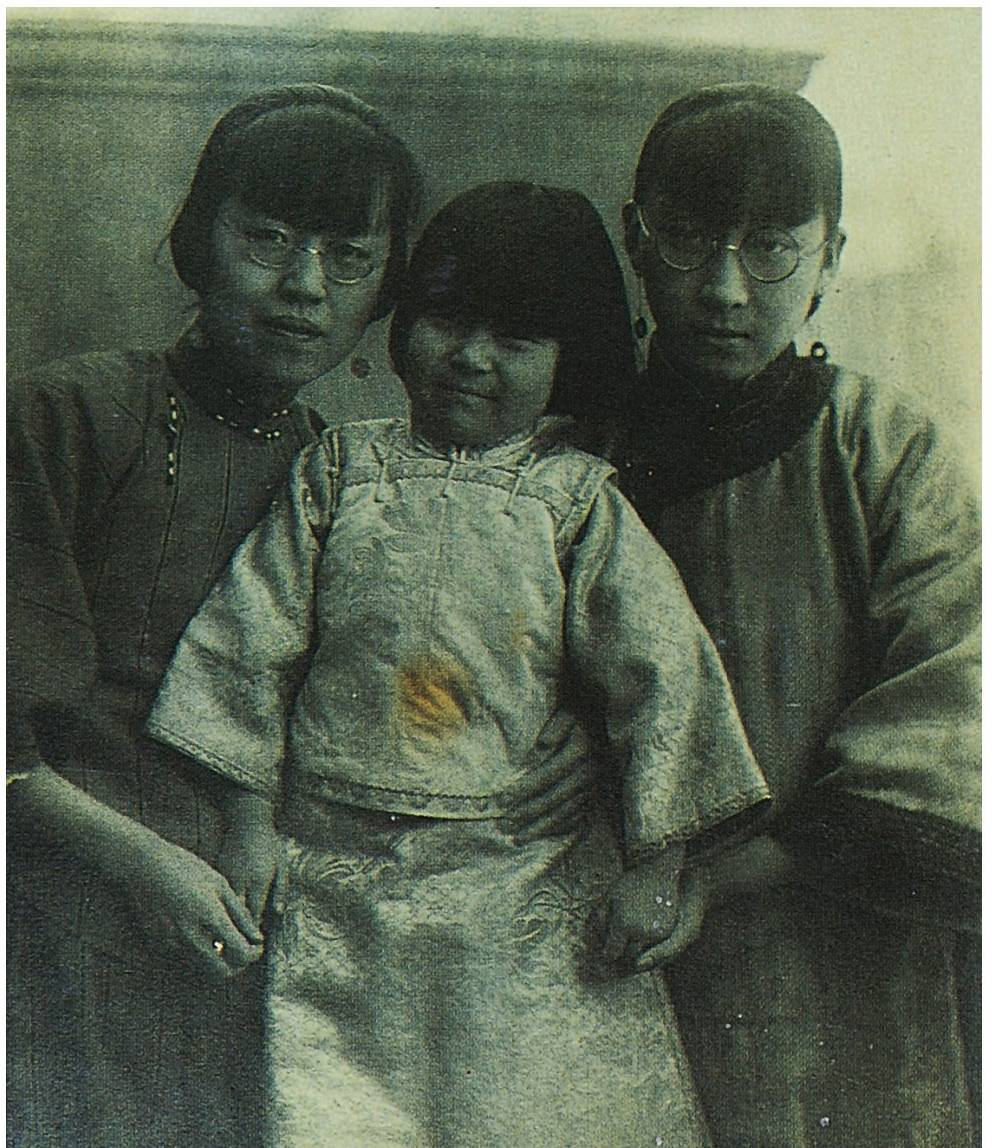
\includegraphics[scale=0.4]{picture/对照记1.jpeg}
\end{figure}


\par 【图二】面团团的,我自己都不认识了。但是不是我又是谁呢?把亲戚间的小女孩都想遍了,全都不像。倒是这张藤几很眼熟,还有这件衣服——不过我记得的那件衣服是淡蓝色薄绸,印着一蓬蓬白雾。T字形白绸领,穿着有点傻头傻脑的,我并不怎么喜欢,只感到亲切。随又记起那天我非常高兴,看见我母亲替这张照片着色。一张小书桌迎亮搁在装着玻璃窗的狭窄的小洋台上,北国的阴天下午,仍旧相当幽暗。我站在旁边看着,杂乱的桌面上有黑铁水彩画颜料盒,细瘦的黑铁管毛笔,一杯水。她把我的嘴唇画成薄薄的红唇,衣服也改填最鲜艳的蓝绿色。那是她的蓝绿色时期。
\par 我第一本书出版,自己设计的封面就是整个一色的孔雀蓝,没有图案,只印上黑字,不留半点空白,浓稠得使人窒息。以后才听见我姑姑说我母亲从前也喜欢这颜色,衣服全是或深或浅的蓝绿色。我记得墙上一直挂着的她的一幅油画习作静物,也是以湖绿色为主。遗传就是这样神秘飘忽——我就是这些不相干的地方像她,她的长处一点都没有,气死人。
\begin{figure}[htb]
    \centering %
    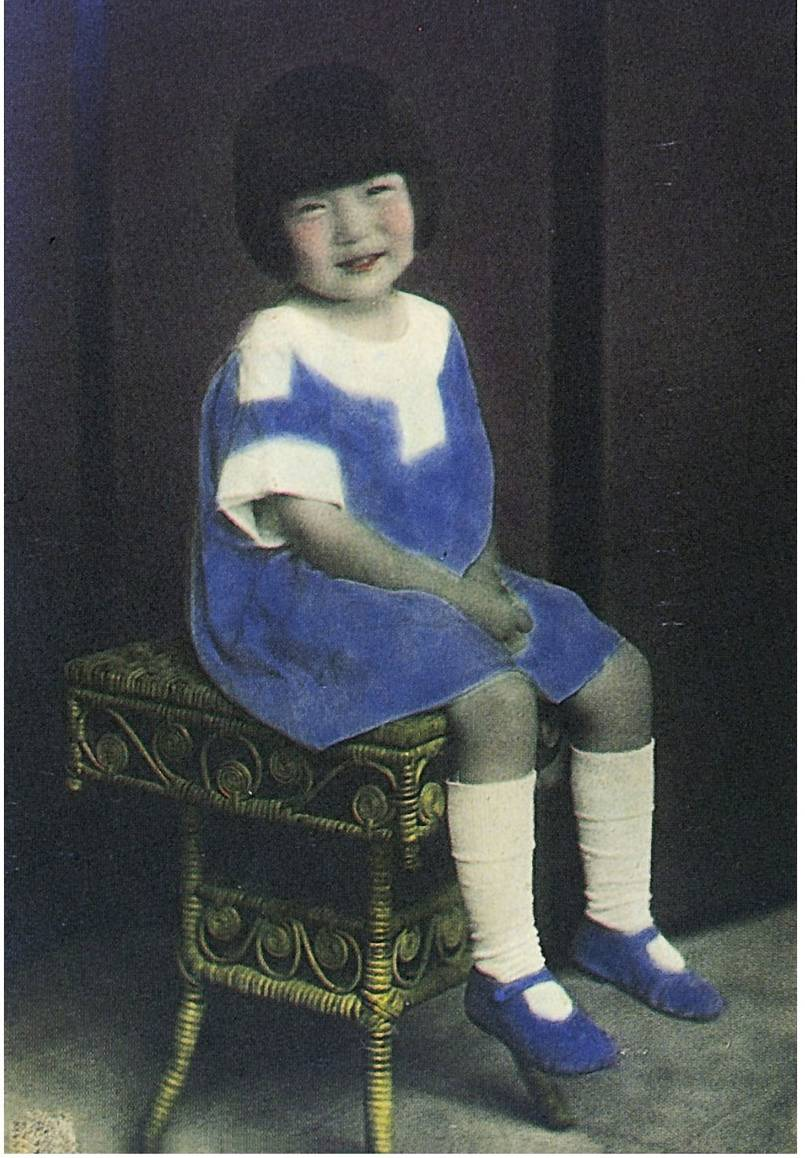
\includegraphics[scale=0.4]{picture/对照记2.jpeg}
\end{figure}

\par 【图三】在天津家里,一个比较简朴的半旧花园洋房,没草坪。戴眼镜的是我父亲,我姑姑,余为我母亲与两个“大侄侄”,妞儿的弟兄们。
\par 我母亲故后遗物中有我父亲的一张照片,被我丢失了。看来是直奉战争的时候寄到英国去的,在照相馆的硬纸夹上题了一首七绝,第一、第三句我只记得开首与大意:
\par 才听津门(“金甲鸣”?是我瞎猜,“鸣”字大概也不押韵。)
\par 又闻塞上鼓鼙声
\par 书生(自愧只坐拥书城?)
\par 两字平安报与卿
\par 因为他娶了妾,又吸上鸦片,她终于藉口我姑姑出国留学需要女伴监护,同去英国,一去四年。他一直催她回来,答应戒毒,姨太太也走了。回来也还是离了婚。她总是叫我不要怪我父亲。


\par 【图四】我喜欢我四岁的时候怀疑一切的眼光。
\par 我母亲与姑姑去后,妞大侄侄与她众多的弟兄们常常轮流来看我和我弟弟,写信去告诉她们。
\par 不光是过年过节,每隔些时老女仆也带我到他们家去。我弟弟小时候体弱多病,所以大都是我一个人去。路远,坐人力车很久才到。冷落偏僻的街上,整条街都是这一幢低矮的白泥壳平房,长长一带白墙上一扇黝黑的原木小门紧闭。进去千门万户,穿过一个个院落与院子里阴暗的房间,都住着投靠他们的亲族。虽然是传统的房屋的格式,简陋得全无中国建筑的特点。
\par 房间里女眷站起来向我们微笑着待招呼不招呼,小户人家被外人穿堂入户的窘笑。大侄侄们一个都不见。带路的仆人终于把我们领到了一个光线较好的小房间。一个高大的老人永远坐在藤躺椅上,此外似乎没什么家具陈设。
\par 我叫声“二大爷。”
\par “认多少字啦?”他总是问。再没第二句话。然后就是“背个诗我听。”“再背个。”
\par 还是我母亲在家的时候教我的几首唐诗,有些字不认识,就只背诵字音。他每次听到“商女不知亡国恨,隔江犹唱后庭花”就流泪。
\par 他五十几岁的瘦小的媳妇小脚伶仃站在房门口伺候。他问了声“有什么吃哒?”她回说“有包子,有盒子。”他点点头,叫我“去玩去。”
\par 她叫了个大侄侄来陪我,自去厨下做点心。一大家子人的伙食就是她一个人上灶,在旁边帮忙的女佣不会做菜。
\par “革命党打到南京,二大爷坐只箩筐在城墙上缒下去的,”我家里一个年轻的女佣悄悄笑着告诉我。她是南京人。
\par 多年后我才恍惚听见说他是最后一个两江总督张人骏。一九六〇初,我在一个美国新闻记者写的端纳传(《中国的端纳》,Donald of China)上看到总督坐箩筐缒出南京围城的记载,也还不十分确定是他,也许因为过去太熟悉了,不大能接受。书中写国民政府的端纳顾问初到中国,到广州去见他,那时候他是两广总督。端纳贡献意见大发议论,他一味笑着直点头,帽子上的花翎乱颤。那也是清末官场敷衍洋人的常态。
\par “他们家穷因为人多,”我曾经听我姑姑说过。
\par 仿佛总比较是多少是个清官,不然何至于一寒至此。
\par 我姑姑只愤恨他把妞大侄侄嫁给一个肺病已深的穷亲戚,生了许多孩子都有肺病,无力医治。妞儿在这里的两张照片上已经定了亲。


\par 【图五】我弟弟这张照片背面印着英文明信片款式,显然是我母亲在英国的时候拿去制成明信片。这一张与她所有的着色的照片都是她自己着色的。



\par 【图六】我们抱着英国寄来的玩具。他戴着给他买的草帽。




\par 【图七】在天津的法国公园。




\par 【图八】我们搬到上海去等我母亲、我姑姑回国。我舅舅家住在张家浜(音“邦”,俗字——近江海的水潭),未来的大光明戏院后面的卡尔登戏院后首的一个不规则的小型广场。叫张家浜,显然还是上海滩初开埠时节的一块沼泽地,后来填了土,散散落落造了几幢大洋房。年代久了,有的已经由住宅改为小医院。街口的一幢,楼下开了个宝德照相馆,也是曾经时髦过的老牌照相馆。我舅母叫三个表姐与表弟带我去合拍张照。
\par 隆冬天气没顾客上门,冰冷的大房间,现在想起来倒像海派连台本戏的后台,墙上倚立着高大的灰尘满积的布景片子。
\par 五个小萝卜头我在正中。还有个表妹最小,那天没去。她现在是电视明星张小燕的母亲。



\par 【图九】我母亲与姑姑回国后和两个表伯母到杭州游西湖,也带了我跟我弟弟去。这是九溪十八涧。


\par 【图十】我外婆是农家女,嫁给将门之子作妾——他父亲是湘军水师。她大概是他们原籍湖南长沙附近的人。他们俩都只活到二十几岁,孩子是嫡母带大的。



\par 【图十一】民初妇女大都是半大脚,裹过又放了的。我母亲比我姑姑大不了几岁,家中同样守旧,我姑姑就已经是天足了,她却是从小缠足。(见图。背后站着的想必是婢女。)踏着这双三寸金莲横跨两个时代,她在瑞士阿尔卑斯山滑雪至少比我姑姑滑得好。(我姑姑说。)
\par 她是个学校迷。我看茅盾的小说《虹》中三个成年的女性入学读书就想起她,不过在她纯是梦想与羡慕别人。后来在欧洲进美术学校,太自由散漫不算。一九四八年她在马来亚侨校教过半年书,都很过瘾。
\par 她画油画,跟徐悲鸿蒋碧微常书鸿都熟识。
\par 珍珠港事变后她从新加坡逃难到印度,曾经做尼赫鲁的两个姐姐的秘书。一九五一年在英国又一度下厂做女工制皮包。连我姑姑在大陆收到信都有点不知道说什么好,只向我悄悄笑道:“这要是在国内,还说是爱国,破除阶级意识——”
\par 她信上说想学会裁制皮革,自己做手袋销售。早在一九三六年她绕道埃及与东南亚回国,就在马来亚买了一洋铁箱碧绿的蛇皮,预备做皮包皮鞋。上海成了孤岛后她去新加坡,丢下没带走。我姑姑和我经常拿到屋顶洋台上去曝晒防霉烂,视为苦事,虽然那一张张狭长的蕉叶似的柔软的薄蛇皮实在可爱。她战后回国才又带走了。
\par 我小时候她就自己学会做洋裁,也常见她车衣。但是她做皮包卖的计划似乎并未成功,来信没再提起。当时不像现在欧美各大都市都有青年男女沿街贩卖自制的首饰等等,也有打进高价商店与大百货公司的。后工业社会才能够欣赏独特的新巧的手工业。她不幸早了二三十年。
\par 她总是说湖南人最勇敢。



\par 【图十二】我母亲,一九二〇初叶在北京。



\par 【图十三】在伦敦,一九二六。



\par 【图十四、十五】一九三〇初在西湖赏梅。




\par 【图十六、十七】三〇中叶在法国。





\par 【图十八】三〇末叶在海船上。



\par 【图十九】我母亲离婚后再度赴欧,我姑姑搬到较小的公寓。本来两人合租的公寓没住多久,迁出前在自己设计的家具地毯上拍照留念。



\par 【图二十】在我姑姑的屋顶洋台上。她央告我“可不能再长高了。”
\par 她在照片背面用铅笔写着:
\par “我这张难看极了小[插图]很自然所以寄给你看看
\par 这地方是气车间顶上小孩顽的地方
\par 我们头顶上的窗就是我的Sitting room的。”
\par 显然是她寄给我母亲同一照片寄出的一张上题字的底稿。
\par 我再稍大两岁她就告诉我她是答应我母亲照应我的。她需要声明,大概也是怕我跟她比跟我母亲更亲近,成了离间亲子感情。
 


\par 【图二十一】我穿着我继母的旧衣服。她过门前听说我跟她身材相差不远,带了两箱子嫁前衣来给我穿。
\par 她父亲孙宝琦以遗老在段祺瑞执政时出任总理,即在北洋政府也算是“官声不好”的,不知怎么后来仍旧家境拮据。总不见得又是因为“家里人多”?他膝下有八男十六女。妻女都染上了阿芙蓉癖。我继母是陆小曼的好友,两人都是吞云吐雾的芙蓉仙子。婚后床头挂着陆小曼画的油画瓶花。她跟“赵四风流朱五狂”的朱氏姊妹也交好,谢媒酒在家里请客,她们也在座。
\par 她说她的旗袍“料子都很好的”,但是有些领口都磨破了。只有两件蓝布大褂是我自己的。在被称为贵族化的教会女校上学,确实相当难堪。学校里一度酝酿着要制定校服,有人赞成,认为泯除贫富界限。也有人反对,因为太整齐划一了丧失个性,而且清寒的学生又还要多出一笔校服费。议论纷纷,我始终不置一词,心里非常渴望有校服,也许像别处的女生的白衬衫、藏青十字交叉背带裙,洋服中的经典作,而又有少女气息。结果学校当局没通过,作罢了。
\par 一九六〇初叶我到台湾,看见女学生清一色的草黄制服,觉得比美国的女童军的墨绿制服帅气,有女兵的英姿。后来在台湾报上看到群情愤激要求废除女生校服,不禁苦笑。
\par 我这论调有点像台湾报端常见的“你们现在多么享福,我们从前吃番薯签”,使年青人听多了生厌。不过我那都是因为后母赠衣造成一种特殊的心理,以至于后来一度clothes-crazy(衣服狂)。



\par 【图二十二】我祖母十八岁的时候与她母亲合影。她仿佛忍着笑,也许是笑钻在黑布下的洋人摄影师。
\par 我弟弟永远比我消息灵通。我住读放月假回家,一见面他就报告一些亲戚的消息。有一次他仿佛抢到一则独家新闻似地,故作不经意地告诉我:“爷爷名字叫张佩纶。”
\par “是哪个佩?哪个纶?”
\par “佩服的佩。经纶的纶,绞丝边。”
\par 我很诧异这名字有点女性化,我有两个同学名字就跟这差不多。
\par 不知道别处风俗怎样,我们祭祖没有神主牌,供桌上首只摆一排盖碗,也许有八九个之多。想必总有曾祖父母。当时不知道祖父还有两个前妻与一个早死的长子,只模糊地以为还再追溯到高祖或更早。偶尔听见管祭祀的老仆嘟囔一声某老姨太的生日,靠边加上一只盖碗,也不便问。他显然有点讳言似地,当着小孩不应当提姨太太的话,即使是陈年八代的。每逢“摆供”,他就先一天取出香炉蜡台桌围与老太爷老太太的遗像,挂在墙上。祖母是照片,祖父是较大的油画像。我们从小看惯了,只晓得是爷爷奶奶,从来没想到爷爷也有名字。
\par 又一天我放假回来,我弟弟给我看新出的历史小说《孽海花》,不以为奇似地撂下一句:“说是爷爷在里头。”
\par 厚厚的一大本,我急忙翻看,渐渐看出点苗头来,专拣姓名音同字不同的,找来找去,有两个姓庄的。是嫖妓丢官后,“小红低唱我吹箫”,在湖上逍遥的一个?看来是另一个,庄[插图]樵,也是“文学侍从之臣”,不过兼有言官的职权,奏参大员,参一个倒一个,一时满朝侧目。李鸿章——忘了书中影射他的人物的名字——也被他参过,因而“褫去黄马褂,拔去三眼花翎。”
\par 中法战争爆发,因为他主战,忌恨他的人就主张派他去,在台湾福建沿海督师大败,大雨中头上顶着一只铜脸盆逃走。
\par 李鸿章爱才不念旧恶,他革职充军后屡次接济他,而且终于把他弄了回来,留在衙中作记室。有一天他在签押房里惊鸿一瞥看见东家如花似玉的女儿,此后又有机会看到她作的一首七律,一看题目《鸡笼》,先就怵目惊心:
\par “鸡笼南望泪潸潸,闻道元戎匹马还。一战何容轻大计,四方从此失边关。……”
\par 李鸿章笑着说了声“小女涂鸦”之类的话安抚他,却着人暗示他来求亲,尽管自己太太大吵大闹,不肯把女儿嫁给一个比她大二十来岁的囚犯。
\par 我看了非常兴奋,去问我父亲,他只一味辟谣,说根本不可能在签押房撞见奶奶。那首诗也是捏造的。
\par 我也听见过他跟访客讨论这部小说,平时也常跟亲友讲起“我们老太爷”,不过我旁听总是一句都听不懂。大概我对背景资料知道得太少。而他习惯地衔着雪茄烟环绕着房间来回踱着,偶尔爆出一两句短促的话,我实在听不清楚,客人躺在烟铺上自抽鸦片,又都只微笑听着,很少发问。
\par 对子女他从来不说什么。我姑姑我母亲更是绝口不提上一代。他们在思想上都受五四的影响,就连我父亲的保守性也是有选择性的,以维护他个人最切身的权益为限。
\par 我母亲还有时候讲她自己家从前的事,但是她憎恨我们家。当初说媒的时候都是为了门第葬送了她一生。
\par “问这些干什么?”我姑姑说。“现在不兴这些了。我们是叫没办法,都受够了,”她声音一低,近于喃喃自语,随又换回平常的声口:“到了你们这一代,该往前看了。”
\par “我不过是因为看了那本小说觉得好奇,”我不好意思地分辩。
\par 她讲了点奶奶的事给我听。她从小父母双亡,父亲死得更早。“爷爷一点都不记得了。”她断然地摇了摇头。
\par 我称大妈妈的表伯母,我一直知道她是李鸿章的长孙媳,不过不清楚跟我们是怎么个亲戚。那时候我到她家去玩,总看见电话旁边的一张常打的电话号码表,第一格填写的人名是曾虚白,我只知道是个作家,是她娘家亲戚。原来就是《孽海花》作者曾孟朴的儿子!
\par 她哥哥是诗人杨云史,他们跟李家是亲上加亲。曾家与李家总也是老亲了,又来往得这样密切。《孽海花》里这一段情节想必可靠,除了小说例有的渲染。
\par 因为是我自己“寻根”,零零碎碎一鳞半爪挖掘出来的,所以格外珍惜。
















































\subsection{编辑之痒}


\par 前两天看到《皇冠》十二月号连载的拙著《对照记》(中),文内自诩沉默寡言而“言必有中”。这一段原文是:
\par “事实是我从来没脱出那‘尴尬的年龄’(the awkward age),不会待人接物,不会说话。话虽不多,‘夫人不言,言必有’失。”
\par 本来末了没引语号,只是
\par “夫人不言,言必有失。”
\par 宋淇教授看了原稿来信说“夫人”会被误认为自称夫人太太。我回信说我本来也担心不清楚,加上引语号,表明是引四书上这句名言,只更动一个字,就绝对不会误会了。不料函札往返讨论了半天,刊出后赫然返璞归真成为:
\par “夫人不言,言必有中。”
\par 自嘲变成自吹自捧,尤其是认识我的人都知道我说话往往不得当,说我木讷还不服,大言不惭令人齿冷。
\par 上一期刊出的还有地名张家浜改为张家滨,当是因为“兵”“宾”同声,以为我嫌“滨”字笔画太多,独创一个简体字“浜”代替它。
\par “浜”这俗字音“邦”,大概是指江边或海边的水潭。上海人称Pidgin English为“洋泾浜”英文——洋人雇用的中国跑街仆役自成一家的英语,如“赶快”称chop-chop,“午餐”称“剔芬”(tiffin),后者且为当地外侨采用。我小时候一直听见我父亲说“剔芬”,直到十几岁才知道英文“午餐”是“冷吃”(lunch)不是“剔芬”。“芬”想必就是“饭”,“剔”不知道是中国何地方言。这一种语言是五口通商以来或更早的十八世纪广州十三行时代就逐渐形成的,还有葡萄牙话的痕迹。
\par 英文名言有“编辑之痒”(editorial itch)这名词。编辑手痒,似比“七年之痒”还更普遍,中外皆然。当然“浜”改“滨”,“言必有失”改“言必有中”不过是尽责的编者看着眼生就觉得不妥,也许礼貌地归之于笔误,径予改正。在我却是偶有佳句,得而复失,就像心口戳了一刀。明知一言既出,驷马难追,何况白纸黑字,读者先有了个印象,再辨正也晚了。
\par  
\par *初载一九九三年十二月二十八日《联合报》副刊,未收集。



\subsection{四十而不惑}


\par 皇冠纪念四十周年,编者来信要我写个祝福的小故事。我想来想去没有。
\par 最初听到祝福这件事,是《圣经》上雅各的哥哥必须要老父祝福他,才有长子继承权,能得到全部家产。父亲对子女有祝福的威权,诅咒也一样有效。中国人的“善颂善祷”就只是说吉利话希望应验。我从前看鲁迅的小说《祝福》就一直不大懂为什么叫“祝福”。祭祖不能让寡妇祥林嫂上前帮忙——晦气。这不过是负面的影响。祭祀祈求祖宗保佑,也只能暗中保佑,没有祝福的仪式。
\par 西方现在也只有开玩笑地或是老太太们表示感谢,轻飘地说声“上帝保佑!”或是“保佑你!”从来不好意思说整句的“上帝保佑你。”
\par 中国人倒是说“四十而不惑。”西方人也说“生命在四十岁开始。”不老也还是要“不惑”才禁得起风险。世变方殷,变得越来越快。皇冠单凭它磨练出的眼光也会在转瞬沧海桑田间找到它自己的路,走向更广阔的地平线。
\par  
\par *初载一九九四年二月《皇冠》第四百八十期,未收集。



\subsection{忆西风\\\small{——第十七届时报文学奖特别成就奖得奖感言}}

\par 得到《时报》的文学特别成就奖,在我真是意外的荣幸。这篇得奖感言却难下笔。三言两语道谢似乎不够恳切。不知怎么心下茫然,一句话都想不出来。但是当然我知道为什么,是为了从前《西风》的事。
\par 一九三九年冬——还是下年春天?——我刚到香港进大学,《西风》杂志悬赏征文,题目是《我的……》,限五百字。首奖大概是五百元,记不清楚了。全面抗战刚开始,法币贬值还有限,三元兑换一元港币。
\par 我写了篇短文《我的天才梦》,寄到已经是孤岛的上海。没稿纸,用普通信笺,只好点数字数。受五百字的限制,改了又改,一遍遍数得头昏脑胀。务必要删成四百九十多个字,少了也不甘心。
\par 法国修道院办的女生宿舍,每天在餐桌上分发邮件。我收到杂志社通知说我得了首奖,就像买彩票中了头奖一样。宿舍里同学只有个天津来的蔡师昭熟悉中文报刊。我拿给她看,就满桌传观。本地的女孩都是圣斯提反书院毕业的,与马来西亚侨生同是只读英文,中文不过识字,不大注意这些。本地人都是阔小姐,内中周妙儿更是父亲与何东爵士齐名,只差被英廷封爵的“太平绅士”(这名词想必来自香港的太平山),买下一个离岛盖了别墅,她请全宿舍的同学去玩一天。这私有的青衣岛不在渡轮航线内,要自租小轮船,来回每人摊派十几块钱的船钱。我就最怕在学费膳宿与买书费外再有额外的开销,头痛万分,向修女请求让我不去,不得不解释是因为父母离异,被迫出走,母亲送我进大学已经非常吃力等等。修女也不能作主,回去请示,闹得修道院长都知道了。连跟我同船来的锡兰朋友炎樱都觉得丢人,怪我这点钱哪里也省下来了,何至于。我就是不会撑场面。
\par 蔡师昭看在眼里,知道我虽然需要钱,得奖对于我的意义远大过这笔奖金,也替我庆幸。她非常稳重成熟,看上去总有二十几岁了。家里替她取名师昭,要她效法著《女训》的班昭,显然守旧。她是过来人,不用多说也能明白我的遭遇。
\par 不久我又收到全部得奖名单。首奖题作《我的妻》,作者姓名我不记得了。我排在末尾,仿佛名义是“特别奖”,也就等于西方所谓“有荣誉地提及(honorable mention)”。我记不清楚是否有二十五元可拿,反正比五百字的稿酬多。
\par 《我的妻》在下一期的《西风》发表,写夫妇俩认识的经过与婚后贫病的挫折,背景在上海,长达三千余字。《西风》始终没提为什么不计字数,破格录取。我当时的印象是有人有个朋友用得着这笔奖金,既然应征就不好意思不帮他这个忙,虽然早过了截稿期限,都已经通知我得奖了。
\par “我们中国人!”我对自己苦笑。
\par 幸而还没写信告诉我母亲。
\par “不是头奖。”我讪讪地笑着把这份通知单给蔡师昭看。其实不但不是头奖,二奖三奖也都不是。我说话就是这样乏。
\par 她看了也只咕哝了一声表示“怎么回事?”,没说什么,脸上毫无表情。她的一种收敛克制倒跟港大的英国作风正合适。她替我难堪,我倒更难堪了。
\par 下学期她回天津去进辅仁大学,我们也没通讯。
\par 《西风》从来没有片纸只字向我解释。我不过是个大学一年生。征文结集出版就用我的题目《天才梦》。
\par 五十多年后,有关人物大概只有我还在,由得我一个人自说自话,片面之词即使可信,也嫌小器,这些年了还记恨?当然事过境迁早已淡忘了,不过十几岁的人感情最剧烈,得奖这件事成了一只神经死了的蛀牙,所以现在得奖也一点感觉都没有。隔了半世纪还剥夺我应有的喜悦,难免怨愤。现在此地的文艺奖这样公开评审,我说了出来也让与赛者有个比较。
\par  
\par *初载一九九四年十二月三日《中国时报·人间》,未收集。




\subsection{笑纹后记}

\par 洛杉矶时报有个副刊题名View(观赏),兼收社交时装占星,以及妇女问题信箱,书评与连环图画。一九九四年五月改名Life and Style(生活与时尚),将流行名词lifestyle(生活作风,一般专指豪华或放浪的生活作风)一分为二,既浑成又俏皮。又新辟一个笑话专栏Laugh Lines,要读者听见什么笑话就寄给他们。我不是订户,只隔几天买份报,所以不太确定副刊改名的日期,反正大概是五月。
\par 在这以前一年,一九九三年三月号的皇冠登载我这篇《笑纹》,文内说笑话专栏可以叫Laugh Lines。现在洛杉矶华人多,不是不可能有皇冠读者向这美西第一大报建议采用这名称。当然也无法指控他们抄袭,只能相信纯属巧合。倒是我需要声明我不是剽窃。
\par 顺便再提一声,这里的五篇散文前三篇是一九四四年的作品。头两篇是我将《倾城之恋》小说改编为舞台剧,上演时写的。
\par  
\par *据手稿。




\subsection{重访边城}


\par 我回香港去一趟,顺便弯到台湾去看看。在台北下飞机的时候,没预备有认识的人来接。我叫麦先生麦太太不要来,因为他们这一向刚巧忙。但是也可能他们托了别人来接机,所以我看见一个显然干练的穿深色西装的人走上前来,并不感到诧异。
\par “你是李察·尼克逊太太?”他用英语说。
\par 我看见过金发的尼克逊太太许多照片,很漂亮,看上去比她的年龄年青二三十岁。我从来没以为我像她,而且这人总该认得出一个中国女同胞,即使戴着太阳眼镜。但是因为女人总无法完全不信一句谀词,不管多么显与事实不符,我立刻想起尼克逊太太瘦,而我无疑地是瘦。也许他当作她戴了黑色假发,为了避免引起注意?
\par “不是,对不起,”我说。
\par 他略一颔首,就转身再到人丛中去寻找。他也许有四十来岁,中等身材,黑黑的同字脸,浓眉低额角,皮肤油腻,长相极普通而看着很顺眼。
\par 我觉得有点奇怪,尼克逊太太这时候到台湾来,而且一个人来。前副总统尼克逊刚竞选加州州长失败,在记者招待会上说了句气话:“此后你们没有尼克逊好让你们踢来踢去了。”显然自己也以为他的政治生命完了。正是韬光养晦的时候,怎么让太太到台湾来?即使不过是游历,也要避点嫌疑。不管是怎么回事,总是出了点什么差错,才只有这么一个大使馆华人干员来接她。
\par “你们可晓得尼克逊太太要来?”我问麦氏夫妇。他们到底还是来了。
\par “哦?不晓得。没听见说。”
\par 我告诉他们刚才那人把我误认作她的笑话。麦先生没有笑。
\par “唔。”然后他有点不好意思地说:“有这么个人老是在飞机场接飞机,接美国名人。有点神经病。”
\par 我笑了起来,随即被一阵抑郁的浪潮淹没了,是这孤岛对外界的友情的渴望。
\par 一出机场就有一座大庙,正殿前一列高高的白色水泥台阶,一个五六十岁的太太相当费劲地在往上爬,裹过的半大脚,梳着髻,臃肿的黑旗袍的背影。这不就是我有个中学同班生的母亲?麦先生正在问我“回来觉得怎么样?”我惊异地微笑,说:“怎么都还在这儿?当是都没有了嘛!”除了年光倒流的感觉,那大庙几乎直盖到飞机场里,也增加了时空的混乱。当时没想到,送行怕飞机失事,要烧香求菩萨保佑,就像渔村为了出海打渔危险,必定要有妈祖庙一样。
\par 我以前没到过台湾,但是珍珠港事变后从香港回上海,乘的日本船因为躲避轰炸,航线弯弯扭扭的路过南台湾,不靠岸,远远的只看见个山。是一个初夏轻阴的下午,浅翠绿的欹斜秀削的山峰映在雪白的天上,近山脚没入白雾中。像古画的青绿山水,不过纸张没有泛黄。倚在船舷上还有两三个乘客,都轻声呼朋唤友来看,不知道为什么不敢大声。我站在那里一动都不动,没敢走开一步,怕错过了,知道这辈子不会再看见更美的风景了。当然也许有更美的,不过在中国人看来总不如——没这么像国画。
\par 轮船开得不快,海上那座山维持它固定的姿势,是否有好半天,还是不过有这么一会工夫,我因为实在贪看,唯恐下一分钟就没有了,竟完全没数,只觉得在注视,也不知道是注入还是注出,仿佛一饮而尽,而居然还在喝,还在喝,但是时时刻刻都可能发现衔着空杯。末了它是怎样远去或是隐没的,也不记得了,就那一个永远忘不了的印象。这些年后到台湾来,根本也没打听那是什么山。我不是登山者,也不想看它陆地上的背面。还是这样好。
\par “台北不美,不过一出城就都非常美,”麦先生在车上说。
\par 到处是骑楼,跟香港一样,同是亚热带城市,需要遮阳避雨。罗斯福路的老洋房与大树,在秋暑的白热的阳光下树影婆娑,也有点像香港。等公车的男女学生成群,穿的制服乍看像童子军。红砖人行道我只在华府看到,也同样敝旧,常有缺砖。不过华盛顿的街道太宽,往往路边的两层楼店面房子太萎琐,压不住,四顾茫茫一片荒凉,像广场又没有广场的情调,不像台北的红砖道有温暖感。
\par 麦氏夫妇知道我的脾气,也不特地请吃饭招待,只作了一些安排。要看一个陌生的城市,除了步行都是走马看花。最好是独行,但是像我这样不识方向的当然也不能一个人乱走。
\par 午后麦太太开车先送麦先生上班,再带我到画家席德进那里去。麦太太是美国人,活泼泼地把头一摔,有点赌气地说:“他是我最偏爱的一个人。(He's my favorite person.)”
\par 她在大门口楼梯脚下哇啦一喊,席先生打着赤膊探头一看,有点不好意思地去穿上衬衫再招呼我们上楼。楼上虽然闷热,布置得简单雅洁,我印象中原色髹漆的板壁很多,正是挂画的最佳背景。走廊就是画廊。我瞻仰了一会,太热,麦太太也没坐下就走了,席先生送她出去,就手陪我去逛街。
\par 有席德进带着走遍大街小巷,是难求的清福。他默无一语,简直就像你一个人逍遥自在地散步,不过免除迷路的恐慌。钻进搭满了晾衣竿的狭巷,下午湿衣服都快干了,衣角偶而微凉,没有水滴在头上。盘花金色铁窗内望进去,小房间里的单人床与桌椅一览无余,浅粉色印花挂衣袋是美国没有的。好像还嫌不够近,一个小女孩贴紧了铁栅站在窗台上,一动也不动地望着我们挨身走过。也许因为房屋轻巧新建,像挤电梯一样挤得不郁塞,仿佛也同样是暂时的。
\par 走过一个花园洋房,灰色砖墙里围着相当大的一块空地,有两棵大树。
\par “这里有说书的。时候还没到,”他说。
\par 想必是露天书场,藤椅还没搬出来。比起上海的书场来,较近柳敬亭原来的树下或是茶馆里说书。没有粽子与苏州茶食,茶总有得喝?要经过这样的大动乱,才摆脱了这些黏附物——零食;雪亮的灯光下,两边墙上橱窗一样大小与位置的金框大镜,一路挂到后座,不但反映出台上的一颦一笑,连观众也都照得清清楚楚。大概为了时髦妓女和姨太太们来捧场,听完了一档刚下场就袅袅婷婷起身离去,全场瞩目,既出风头又代作广告。
\par 经过一座庙,进去随喜。这大概是全世界最家常的庙宇,装着日光灯,挂着日历。香案上供着蛋杯——吃煮蛋用的高脚小白磁杯,想是代替酒盅。拜垫也就用沙发上的荷叶边软垫,没有蒲团。墙上挂着个木牌写着一排排的姓名,不及细看,不知是不是捐钱盖庙的施主。
\par 祀的神中有神农,半裸,深棕色皮肤,显然是上古华南居民,东南亚人的远祖。神农尝百草,本来草药也大都是南方出产,北边有许多都没有。草药发明人本来应当是华南人。——是否就是“南药王”?——至于民间怎么会知道史前的华南人这么黑,只能归之于种族的回忆,浩如烟海的迷茫模糊的。我望着那长方脸黝黑得眉目不清的,长身盘腿坐着的神农,败在黄帝手中的蚩尤的上代,不禁有一种森森然的神秘感,近于恐惧。
\par 神案上花瓶里插着塑胶线组成的镂空花朵。又插着一大瓶彩纸令旗,过去只在中秋节的香斗上看见过。该是道教对佛寺的影响。神殿一隅倚着搭戏台用的木材。
\par 下一座庙是个古庙——当然在台北不会太古老。灰色的屋瓦白苍苍的略带紫蓝,色调微妙,先就与众不同。里面的神像现代化得出奇,大头,面目狰狞,帽子上一颗大绒球横斜,武生的戏装;身材极矮,从俯视的角度压缩了。与他并坐的一位索性没有下半身。同是双手搁在桌上,略去下肢的一个是高个子,躯干拉长了,长眉直垂到腮颊上。这决不是受后期印象派影响的现代雕塑,而是当年影响马蒂斯的日本版画的表亲或祖先。日本吸收中国文化,如汉字就有一大部份是从福建传过去的。闽南塑像的这种特色,后来如果失传了,那就是交通便利了些之后,被中原的主流淹没了。(注)
\par 下首大玻璃柜里又有只淡黄陶磁怪龙,上颏奇长,长得像食蚁兽,如果有下颏,就是鳄鱼了,但是缺下颏,就光吐出个舌头。背上生翅,身子短得像四脚蛇。创造怪兽,似乎殷周的铜器之后就没有过?
\par 这么许多疑问,现成有行家在侧,怎么不请教一声?仿佛有人说过,发问也要学问。我脑子一时转不过来,不过看着有点奇怪而已,哪问得出什么。连庙名没看清楚,也都没问是什么庙。多年后根据当时笔记作此文,席德进先生已经去世,要问也没处问了。那天等于梦游症患者,午睡游台北。反正那庙不会离席先生寓所太远,不然我也走不动。
\par 麦家这两天有远客住在他们家,替我在山上的日式旅馆定了个房间,号称“将军套房”,将军上山来常住的。进房要经过一连串的小院子,都有假山石与荷池,静悄悄的一个人影子都不见。在房中只听见黄昏细雨打着芭蕉,还有就是浴室里石狮子嘴里流出的矿泉,从方柜形水泥浴缸口漫出来,泊泊溅在地上。房间里塌塌米上摆着藤家具。床上被单没换,有大块黄白色的浆硬的水渍。显然将军不甘寂寞。如果上次住在这里的是军人。我告诉自己不要太挑剔,找了脚头一块干净土蜷缩着睡,但是有臭虫。半夜里还是得起来,睡在壁龛的底板上——日式客厅墙上的一个长方形浅洞,挂最好的画,摆最好的花瓶的地方。下缘一溜光滑的木板很舒服,也不太凉。一觉睡到日上三竿,女服务生进来铺床,找不到我,吓了一大跳。
\par 幸而只住了一夜。麦家托他们的一个小朋友带我到他家乡花莲观光,也是名城,而且有高山族人。
\par 一下乡,台湾就褪了皮半卷着,露出下面较古老的地层。长途公共汽车上似乎全都是本省人。一个老妇人扎着地中海风味的黑布头巾、穿着肥大的清装袄袴,戴着灰白色的玉镯——台玉?我也算是还乡的复杂的心情变成了纯粹的观光客的游兴。
\par 替我作向导的青年不时用肘弯推推我,急促地低声说:“山地山地!”
\par 我只匆匆一瞥,看到一个纤瘦的灰色女鬼,颊上刺青,刻出蓝色胡须根根上翘,翘得老高,背上背着孩子,在公路旁一爿店前流连。
\par “山地山地!”
\par 吉卜西人似的儿童,穿着破旧的T恤,西式裙子,抱着更小的孩子。
\par “有日本电影放映的时候,他们都上城来了,”他说。
\par “哦?他们懂日文?”
\par “说得非常好。”
\par 车上有许多乘客说日语。这都是早期中国移民,他们的年青人还会说日文的多得使人诧异。
\par 公共汽车忽然停了,在一个“前不巴村,后不巴店”的地方。一个壮硕的青年跳下车去,车掌也跟着下去了。忽然打起架来,两人在地下翻滚。蓝天下,道旁的作物像淡白的芦梗矮篱似的齐臻臻的有二尺高。
\par “契咖茹哟!契咖茹哟!(搞错了哟!)”那青年在叫喊。
\par 司机也下去了,帮着打他。
\par 大概此地民风强悍。一样是中国人,在香港我曾经看见一个车掌跟着一个白坐电车的人下去,一把拉住他的西装领带,代替从前的辫子,打架的时候第一先揪的。但是那不过是推推搡搡辱骂恫吓,不是真动武。这次我从台湾再去香港,有个公车车掌被抓进警察局,因为有个女人指控他用车票打孔机打她。——他们向来总是把那件沉重的铁器临空扳得轧轧响,提醒大家买票。——那也还不是对打。香港这一点是与大陆一致的,至少是提倡“武斗”前的大陆。
\par 这台湾司机与车掌终于放了那青年,回到车上来。
\par “他们说这人老是不买票,总是在这儿跳下去,”我的青年朋友把他们的闽南话译给我听。
\par 挨打的青年站起来拍拍身上的灰尘。他的美军剩余物资的茶褐色衬衫撕破了。公车开走了,开过他身边的时候,他向它立正敬礼。他不会在日据时代当过兵,年纪不够大,但是那种奇异的敬意只有日本有。
\par 观光客大都就看个教堂,在中国就是庙了。花莲的庙比台北还更家庭风味,神案前倚着一辆单车,花瓶里插着鸡毛掸帚。装置得高高的转播无线电放送着流行音乐。后院红砖阑干砌出工字式空花格子,衬着芭蕉,灯影里偶有一片半片蕉叶碧绿。后面厨房里昏黄的灯下,墙上挂着一串玲珑的竹片锁链,蒸馒头用的。我不能想像在蒸笼里怎么用,恨不得带回去拿到高级时装公司去推销,用作腰带。纯棉的瑞士花布如果乱红如雨中有一抹竹青,响应竹制衣带,该多新妍可喜!
\par 花莲城隍庙供桌上的暗红漆茭杯像一副猪腰子。浴室的白磁砖墙。殿前方柱与神座也是白磁砖。横挡在神案前的一张褪色泥金雕花木板却像是古物中的精品。又有一对水泥方柱上刻着红字对联。忽然一抬头看见黑洞洞的天上半轮凉月——原来已经站在个小院子里。南中国的建筑就是这样紧凑曲折,与方方正正的四合院大不相同。月下的别院,不禁使人想起无数的庵堂相会的故事。
\par 此地的庙跟台北一样,供香客插烛的高脚蜡台上都没装铁签——那一定是近代才有的。台湾还是古风,山字架的下截补换了新木,更显出上半的黯黑旧白木棍棒的古拙。有的庙就在木架上架只小藤箩,想必箩中可以站满蜡烛——一只都没有,但是揣度木架的部位与高矮,不会不是烛台。因陋就简,还是当初移民的刻苦的遗风。
\par 还有一个特点是神像都坐在神龛外,绣幔前面。乍看有点看不惯,太没掩蔽,仿佛丧失了几分神秘庄严。想来是神像常出巡,抬出抬进,天气又热,挥汗出力搬扛的人挨挨擦擦,会污损丝绸帐幔。我看见过一张照片上,庙门外挤满了人,一个穿白汗背心的中年男子笑着横抱着个长须神像,脸上的神情亲切,而仿佛不当桩事,并不肃然。此地的神似乎更接近人间,人比在老家更需要神,不但背乡离井,同荒械斗“出草”也都还是不太久以前的事,其间又还经过五十年异族的统治,只有宗教是还是许可的。这里的人在时间与空间上都是边疆居民,所以有点西部片作风。我想起公共汽车旁的打斗。
\par 花莲风化区的庙,荷叶边拜垫上镶着彩色补钉图案,格外女性化些。有一只破了的,垫在个大缸底下。高僧坐化也是在缸中火葬的,但是这里的缸大概是较日常的用途。缸上没有木盖,也许还是装自来水前的水缸。香案前横幅浮雕板上嵌满碎珊瑚枝或是海滩石子作背景。日光灯的青光下,绣花神幔上包着的一层玻璃纸闪闪发光。想必因为天气潮湿,怕丝绸腐烂。
\par 夜间没有香客,当然是她们正忙的时候。殿外大声播送爵士乐,更觉冷冷清清。廊下一群庙祝高坐在一个小平台上,半躺在藤椅上翘着脚喝茶谈天。殿侧堆着锣鼓乐器,有一面大鼓上写着“特级”二字。
\par 附近街上一座简陋的三层楼木屋,看上去是新造的,独门独户站在一小块空地上,门口挂着“甲种妓女户”门牌。窗内灯光雪亮,在放送摇滚乐。靠墙直挺挺两只木椅,此外一无所有。两个年青的女人穿着短旗袍,长头发披在背上,仿佛都是大眼睛高个子高胸脯,足有国际标准,与一个男子在跳摇滚舞。男子近中年了,胖胖的,小眼睛,有点猪相,拱着鼻子,而面貌十分平凡,穿着米色拉链夹克,随和地舒手舒脚,至多可以说跟得上。但是此地明明不是舞校,也许是他们自己人闲着没事做广告。
\par 二等妓院就没有这么纯洁了。公共食堂大观园附设浴堂,想也就是按摩院,但是听说是二等妓院。楼下一排窗户里,有一张藤躺椅上铺着条毛巾被,通内室的门里有个大红织锦缎长旗袍的人影一闪。这样衣冠齐整怎么按摩?似乎与大城市的马杀鸡性质不同。
\par 另一个窗户里有个男子裸体躺在藤椅上,只盖块大毛巾。又有个窗户里,一个人伛偻着在剪脚趾甲。显然不像大陆上澡堂子里有修脚的。既然是自理,倒不省点钱在家里剪,而在这春宵一刻值千金的时候且忙着去剪脚趾甲。虽然刚洗过澡指甲软些容易剪,也是大杀风景的小小豪举。
\par 这一排窗户不知是否隔成小室的统间,下半截墙漆成暗绿色,上半截奶油色,壁上有只老式挂钟。楼下大敞着门,门前停着许多单车,歪歪斜斜互相偎倚着叠放。大门内一列深棕色柜台,像旅馆或医院挂号处。墙壁也漆成同样的阴暗的绿色,英美人称作“医院绿”的。
\par 大概因为气候炎热需要通风,仿佛没有窗帘这样东西,一律开放展览。小电影院也只拉上一半铁门,望进去黑洞洞的一直看到银幕与两旁的淡绿色舞台幕。
\par 风化区的照相馆门口高高下下挂满妓女的照片,有的学影星张仲文长发遮住半边脸,有的像刘琦,都穿着低领口夜礼服。又有同一人两张照片叠印的,清末民初盛行的“对我图”。
\par 夜游后,次日再去看古屋。本地最古老的宅第是个二层楼红砖屋,正楼有飞檐,山墙上镶着湖绿陶磁挖花壁饰,四周簇拥着淡蓝陶磁小云朵。两翼是平房。场院很大,矮竹篱也许是后添的。院门站得远远的,是个小牌楼,上有飞檐,下面一对红砖方柱。
\par 台湾仿佛一直是红砖,大概因为当地的土质。大陆从前都是青砖,其实是深灰色,可能带青灰。因为中国人喜爱青色——“青出于蓝而胜于蓝”——径称为青砖。红砖似是外来的,英国德国最普遍的,条顿民族建筑的特色。在台湾,红砖配上中国传统的飞檐与绿磁壁饰,于不调和中别有一种柔艳憨厚的韵味。
\par 有个嘉庆年间的庙,最古的一翼封闭了,一扇门上挂着木牌,上写“办公处Office”。侧面墙上有个书卷形小窗,两翼各嵌一只湖绿陶磁挖花壁饰作窗棂,中央的一枚想必砸破了,换装三根原木小棍子,也已经年深月久了,予人的感觉是原有的,整个的构图倒更朴拙有致。
\par 又有一幢老屋,普通的窗户也用这种八角形绿磁挖花壁饰作窗棂,六只叠成两行。后加同色木栅保护,褪色的淡蓝木栅也仍旧温厚可爱,没有不调和。
\par 小巷里,摇茶叶的妇人背着孩子在门前平台上席地围坐,大家合捧着个大扁篾篮,不住地晃动着。篮子里黑色的茶叶想必是乌龙,茶香十步外特别浓。另一家平台上堆满了旧车胎。印度也常有这种大门口的平台。
\par 年青的朋友带我来到一处池塘,一个小棕榈棚立在水心。碧清的水中偶有两丛长草倒影。是农场还是渔塭?似乎我的导游永远都是沉默寡言,我不知道怎么也从来不问。
\par 有个长发女郎站在亮蓝的水里俯身操作,一件橙黄桔绿的连衫裙卷到大腿上;面貌身材与那两个甲种妓女同一类型,不过纤巧清扬。除了电影里,哪有这等人物这身打扮作体力劳动的?如果我是贵宾来参观,就会疑心是“波田姆金的村庄”——俄国女皇凯萨琳二世的宠臣波田姆金(Potemkin)在女皇游幸途中遍植精雅的农舍,只有前面一堵假墙,又征集村姑穿着当地传统服装载歌载舞,一片升平气象。
\par 这美人想必引人注目惯了,毫不理会我们眈眈遥视,过了一会,径自趟水进棚去了。我这才微弱地嗳呀了一声,带笑惊叹。那青年得意地笑了。
\par 此地大概是美人多。一来早期移民本来是南国佳人,又有娶山地太太的高山族,至少是花莲的阿美族比著名出美人的峇里人还要漂亮。
\par 我们沿着池边走到一个棕榈凉亭歇息,吃柚子。从来没吃过这样酸甜多汁的柚子,也许因为产地近,在上海吃到湖南柚子早已干了。我望着地下栏杆的阴影里一道道横条阳光。刚才那彩色阔银幕的一场戏犹在目前,疑幻疑真,相形之下,柚子味吃到嘴里真实得使人有点诧异。
\par  
\par 同是边城,香港不像台湾有一水之隔,不但接壤,而且返乡探亲扫墓的来来去去络绎不绝,对大陆自然看得比较清楚。我这次分租的公寓有个大屋顶洋台,晚上空旷无人,闷来就上去走走,那么大的地方竟走得团团转。满城的霓虹灯混合成昏红的夜色,地平线外似有山外山遥遥起伏,大陆横躺在那里,听得见它的呼吸。
\par 二房东太太是上海人,老是不好意思解释他们为什么要分租:“我们都是寄包裹寄穷了呀!”
\par 他们每月寄给她婆家娘家面条炒米咸肉,肉干笋干,砂糖酱油生油肥皂,按季寄衣服。有一种英国制即融方块鸡汤,她婆婆狂喜地来信说它“解决了我们一天两顿饭的一切问题”。砂糖他们用热水冲了吃作为补品。她弟弟在劳改营,为了窝藏一个国特嫌犯;写信来要药片治他的腰子病与腿肿。她妹妹是个医生,派到乡下工作。“她晚上要出诊,乡下地方漆黑,又高低不平,她又怕蛇——女孩子不就是这样。”她抱歉的声口就像是说她的两个女儿占用浴室时间太长,“女孩子不就是这样。”
\par 我正赶上看见他们一次大打包。房东太太有个亲戚要回去,一个七十来岁的老太太,可以替他们带东西。她丈夫像牛仔表演捉小牛,用麻绳套住重物,挣扎得在地板上满地滚。房东太太烤了只蛋糕,又炖了一锅红烧肉。
\par “锅他们也用得着,”她说。
\par “一锅红烧肉怎么带到上海?”我说。
\par “冻结实了呀。火车像冰箱一样。”
\par 她天亮就起来送行,也要帮着拎行李通过罗湖边境的检查。第二天她一看见我就叫喊起来:“哈呀!张小姐,差点回不来喽!”“嗳呀,怎么了?”
\par “嚇咦呀!先不先,东西也是太多,”她声音一低,用串通同谋的口气。“也是这位老太,她自己的东西实在多不过。整桶的火油,整箱的罐头,压成板的咸鱼装箱,衣裳被窝毯子,锅呀水壶,样样都有,够陪嫁摆满一幢房子的。关卡上的人不耐烦起来了。后来查到她皮夹子里有点零钱,人民票,还是她上趟回来带回来的,忘了人民票不许带出来的。夥咦!这就不得了了。‘这是哪来的?哈?’嗯,‘你这是什么意思?啊?’找上我了:‘你是什么人?啊?你跟她是什么关系,哈?你在这干什么,啊?'”房东太太虎起一张孩儿面,竖起一双吊梢眼,吼出那些“啊”“哈”。“嗳呀我说我什么都不知道,我是来送行的——心里嚜一直急得要死。”她皱着眉啧的一声,又把声音一低,窃窃私语道:“这位老太有好几打尼龙袜子缝在她棉袍里。”
\par “带去卖?”
\par “不是,去送礼。女人穿在长袴里。”
\par “——看都看不见!”
\par “不是长统的。”她向她小腿上比划了一下。“送给干部太太。她总喜欢谁都送到。好能干呵,老太。她把香港拍的电影进口。给高干看的。要这么些钱干什么?哈?七十岁了,又没儿女,哈?”她笑了。
\par 这时候正是大跃进后大饥荒大逃亡,五月一个月就有六万人冲出香港边界。大都是邻近地带的乡民。向来是农民最苦,也还是农民最苦。十年前我从罗湖出境的时候,看见乡下人挑着担子卖菜的可以自由出入,还羡慕他们。我们火车上下来的一群人过了罗湖桥,把证件交给铁丝网那边的香港警察。拿了去送到个小屋去研究,就此音信杳然。正是大热天,我们站在太阳地里等着。这香港警察是个瘦长的广东靓仔,戴着新款太阳眼镜,在大陆来的土包子眼中看来奇大的墨镜,穿的制服是短袖衬衫,百慕达短袴,烫得摺痕毕挺,看上去又凉爽又倨傲,背着手踱来踱去。中共站冈的兵士就在我们旁边,一个腮颊圆鼓鼓的北方男孩,穿着稀皱的太大的制服。大家在灼热的太阳里站了一个钟头之后,那小兵愤怒地咕噜了一句,第一次开口:“让你们在外头等着,这么热!去到那边站着。”他用下颏略指了指后面一箭之遥,有一小块阴凉的地方。
\par 我们都不朝他看,只稍带微笑,反而更往前挤近铁丝网,仿佛唯恐遗下我们中间的一个。但是仍旧有这么一刹那,我觉得种族的温暖像潮水冲洗上来,最后一次在身上冲过。
\par 我学生时代的香港,自从港战后回上海,废学十年,那年再回去,倒还没怎么改变,不过校园后面小山上的树长高了,中间一条砖砌小径通向旧时的半山女生宿舍,比例不同了,也有点“面熟陌生”。我正眼都没看它一眼,时间的重量压得我抬不起头来,只觉得那些拔高了的小杉树还有点未成年人的伶仃相,一个个都是暗绿的池中暗绿的喷泉向白色的天上射去,咝咝哗哗地上升,在那一刹那间已经把我抛下很远,缩小了而清晰异常,倒看的望远镜中人,远远的站在地下。没等这画面成形,我早已转身走开了。
\par 这次别后不到十年,香港到处在拆建,邮筒半埋在土里也还照常收件。造出来都是白色大厦,与非洲中东海洋洲任何新兴都市没什么分别。偶有别出心裁的,抽屉式洋台淡橙色与米黄相间,用色胆怯得使人觉得建筑师与画家真是老死不相往来的两族。
\par 想必满山都是白色高楼,半山的杜鹃花早砍光了。我从来没问起。其实花丛中原有的二层楼姜黄老洋房,门前洋台上褪了漆的木柱栏杆,掩映在嫣红的花海中,惨戚得有点刺目,但是配着碧海蓝天的背景,也另有一种凄梗的韵味,免得太像俗艳的风景明信片。
\par 这种老房子当然是要拆,这些年来源源不绝的难民快把这小岛挤坍了,怎么能不腾出地方来造房子给人住?我自己知道不可理喻,不过是因为太喜欢这城市,兼有西湖山水的紧凑与青岛的整洁,而又是离本土最近的唐人街。有些古中国的一鳞半爪给保存了下来,唯其近,没有失真,不像海外的唐人街。
\par 这次来我住在九龙,难得过海,怕看新的渡轮码头,从前光润的半旧枣红横条地板拆了,换了水泥地。本来一条长廊伸出海中,两旁隔老远才有一张玻璃盒装的广告画,冷冷清清介绍香烟或是将上映的影片。这么宝贵的广告空间,不予充份利用,大有谐星的throwing line的风度——越是妙语越是“白扔掉”,不经意地咕哝一声,几乎听不清楚。那一份闲逸我特别欣赏。
\par 相形之下,新盖的较大的水泥建筑粗陋得惨不忍睹。我总是实在非过海不可,才直奔那家店铺,目不斜视。这样谋犹,自然见闻很少。
\par 但是看来南下的外省人已经同化了。孩子们在学校里说广东话,在家里也不肯讲任何其他方言,正好不与父母交谈,别处的十几岁的人也许会羡慕他们有这藉口。
\par 耶诞节他们跟同学当面交换圣诞卡片。社会上不是教徒也都庆祝,送礼,大请客。
\par 报上十三妹写的专栏有个读者来信说:“我今年十九岁。”一年前她父亲带她从华北逃出来,一路经过无数艰险,最后一程子路乘小船到澳门,中途被中共射击,父亲用身体遮着她,自己受了重伤,死在澳门的医院里。她到了香港,由父亲的一个朋友给找了个小事,每月约有一百元港币,只够租一个床位,勉强存活。“全香港只有我不过圣诞节,”她信上说。“请告诉我我是不是应当回大陆去。”
\par 十三妹怎样回答的,不记得了,想必总是劝勉一番。我的反应是漫画上的火星直爆,加上许多“!”与“\#”,不管“\#”在这里是代表什么。当然也不值得这样大惊小怪,在封闭的社会里,年青人的无知,是外间不能想像的。连父母在家里有许多话也都不敢说,怕万一被子女检举。一到了香港的花花世界,十九岁的女孩正是爱美的年龄,想装饰自己的欲望该多强烈。冠盖满京华,斯人独憔悴,是真宁可回到“大家没得”的地方,少受点痛苦。不过一路出来,没有粮票路条,不靠亲友帮忙决走不了这么远。一回去追究起来,岂不害了这些恩人?
\par 我觉得这是个非常好的故事,紧张,悲壮,对人性有讽刺性的结局。可惜我不会写。
\par 临走我有个亲戚约了在香港饭店见一面,晚上七点半在大厅上泡壶红茶,叫了一盘小蛋糕。谈了一会,出来也才八点多。我得要买点廉价金饰带回去送人,听说就在后面一条街上就有许多金铺,开到很晚,顺便去一趟。在饭店门口作别,不往天星码头走,需要解释。表姑父听我说还要去买东西,有点错愕,但是显然觉得我也算是个老香港了,不便说什么,略一点头呵腰,就在灯光黯淡的门廊里一转弯消失了身影。
\par 我循着门廊兜过去,踏上坡斜的后街往上爬,更黑洞洞起来,一个人影子都不见。香港也像美国了,一到了晚上,营业区就成了死城,行人绝迹,只有汽车风驰电掣来往。这青石板山道斜度太陡,不通车,就一片死寂。
\par 到底是中环,怎么这么黑?我该不是第一次发现我有夜盲症,但还是不懂怎么没走过几家门面,顿时两眼漆黑。小时候天色黄昏还在看书,总听见女佣喊叫:“再看要鸡茅(盲?)子眼啦!”“开了灯不行吗?”“开了灯也是一样!”似乎是个禁忌的时辰。只知道狗的视力不佳,鸡是天一黑就看不见了?也许因此一到晚上“鸡栖于埘”,必须回到鸡窝去。照理在光线不足的地方看书,只会近视。黄昏的时候看书就得夜盲症,那是个禁忌的时辰,仿佛全凭联想,不科学。但是事实是我傍晚下台阶就看不清楚梯级,戴着眼镜也没用。不过一向没注意,这下子好!——正赶着这时候壮着胆子不去想香港那些太多的路劫的故事,索性瞎了眼乱闯,给捅一刀也是自讨的。
\par 都怪我不肯多跑一趟,怕过海,要两次并一次,这么晚才去买东西。谁叫你这样感伤起来,我对自己说。就有那么些感情上的奢侈!怕今昔之感,就不要怕匝颈路劫。活该!
\par 道旁该都是些旧式小店,虽然我这次回来没来过。楼上不会不住人,怎么也没有半点灯光?也是我有点心慌意乱,只顾得脚下,以及背后与靠边的一面随时可能来的袭击,头上就不理会了,没去察看有没有楼窗漏出灯光,大概就有也稀少微弱,而且静悄悄的声息毫无。
\par 要防街边更深的暗影中窜出人来,因此在街心只听见石板路的渐渐的脚步声。古老的街道没有骑楼,毕直,平均地往上斜,相当阔,但是在黑暗中可宽可窄,一个黑胡同。预期的一拳一脚,或是一撞,脑后一闷棍,都在蓄势跃跃欲试,似有若无,在黑暗中像风吹着柔软的汽球,时而贴上脸来,又偶一拂过头发,擦身而过,仅只前前后后虚晃一招。
\par 这不是摆绸布摊的街吗?方向相同,斜度相同。如果是的,当然早已收了摊子,一点痕迹都不留。但是那样乡气的市集,现在的香港哪还会有?现在街上摆地摊的只有大陆带出来的字画,挂在墙上。事隔二十年,我又向来不认识路,忘了那条街是在娱乐戏院背后,与这条街平行。但是就在这疑似之间,已经往事如潮,四周成为喧闹的鬼市。摊子实在拥挤,都向上发展,小车柜上竖起高高的杆柱,挂满衣料,把沿街店面全都挡住了。
\par 在人丛里挤着,目不暇给。但是我只看中了一种花布,有一种红封套的玫瑰红,鲜明得烈日一样使人一看就瞎了眼,上面有圆圆的单瓣浅粉色花朵,用较深的粉红密点代表阴影。花下两片并蒂的黄绿色小嫩叶子。同样花还有碧绿地子,同样的粉红花,黄绿叶子;深紫地子,粉红花,黄绿叶子。那种配色只有中国民间有。但是当然,非洲人穿的犷野原始图案的花布其实来自英国曼彻斯特的纺织厂——不过是针对老非洲市场,投其所好。英国人仿制的康熙青花磁几可乱真。但是花洋布不会掉色。与我同去的一个同学用食指蘸了唾沫试过了。是土布。我母亲曾经喜欢一种印白竹叶的青布,用来做旗袍,但是那白竹叶上腻着还没掉光的石膏,藏青地子沾着点汗气就掉色,皮肤上一块乌青像伤痕。就我所知,一九三〇年间就剩这一种印花土布了。香港这些土布打哪来的?如果只有广东有,想必总是广州或是附近城镇织造的。但是谁穿?香港山上砍柴的女人也跟一切广东妇女一样一身黑。中上等妇女穿唐装的,也是黑香云纱衫袴,或是用夏季洋服的浅色细碎小花布。校区与中环没有婴儿,所以一时想不到。买了三件同一个花样的——实在无法在那三个颜色里选择一种——此外也是在这摊子上,还买了个大红粉红二色方胜图案的白绒布,连我也看得出这是婴儿襁褓的料子。原来这些鲜艳的土布是专给乳婴做衣服的,稍大就穿童装了。
\par 广州在清初“十三行”时代——十三个洋行限设在一个小岛上,只准许广州商人到岛上交易——是唯一接近外国的都市,至今还有炸火腿三明治这一味粤菜为证。他们特有的这种土布,用密点绘花瓣上的阴影,是否受日本的影响?我只知道日本衣料设计惯用密圈,密点不确定。如果相同,也该是较早的时候从中国流传过去的,因为日本的传统棉布向来比较经洗,不落色,中国学了绘图的技巧,不会不学到较进步的染料。
\par 看来这种花布还是南宋迁入广东的难民带来的,细水长流,不绝如缕,而且限给乳婴穿。
\par 我从前听我姑姑说:“天津乡下女人穿大红扎脚袴子,真恶心!”那风沙扑面的黄土平原上,天津近海,想必海风扫荡下更是荒瘠不毛之地。人对色彩的渴望,可想而知。但看传统建筑的朱栏,朱门,红楼,丹墀,大红漆柱子,显然中国人是爱红的民族。——虽说“大红大绿”,绿不过是陪衬,因为讲究对称。几乎从来没有单独大块的绿色的——但是因为衣服比房舍更接近个人,大红在新房新妇之外成了禁条。
\par 当时亲戚家有个年纪大的女仆,在上海也仍旧穿北方的扎脚袴。“老李婆的扎脚袴尿臊臭,”我姑姑也听见过这笑话。老年人本来邋塌,帮佣生涯也一切马虎,扎脚袴又聚气。北边乡下缺水,天又冷,不大能洗澡。大红棉袴又容易脏,会有黑隐隐的垢腻痕。也许是尿臊臭的联想加上大红袴子的挑逗性,使我姑姑看了恶心。
\par 唐宋的人物画上常有穿花衣服的,大都是简化的团花,可能并不忠实复制原来的图案。衣服几乎永远是淡赭色或是淡青,石青,石绿。出名的“青衣”“乌衣”从来没有。是否是有一种不成文法的自我约束?
\par 中国固有的丝绸棉布都褪色,所以绝大多数的人在绝大多数的时候都是穿褪色的衣服,正如韩国的传统服装是白色,因为多山的半岛物产不丰,出不起染料钱。中国古画中人物限穿淡赭,石青,石绿,淡青,原来是写实的,不过是褪了色的大红大绿深青翠蓝。中国人最珍爱的颜色。“青出于蓝而胜于蓝”,“红男绿女”——并不是官员才穿大红袍的。后人作画墨守成规,于是画中人穿那寥寥几种轻淡的颜色。当然,这不是说这些冲淡的色调是不适合国画的风格。
\par 明末清初冒辟疆在回忆录中写董小宛“衣退红衫”观潮,众人望之如凌波仙子。我一向以为“退红”是最淡的粉红,其实大概也就是淡赭色,不过身为名妓,她当然只穿新衣,是染就的淡赭红,穿着更亭亭入画。
\par 倒不是绘画的影响,而是满清入关,满人不是爱红的民族,清宫的建筑与室内装修的色调都趋向苍淡,上行下效,一方面物极必反,汉人本来也已穿厌了“鲜衣”。有这句谚语:“若要俏,须带三分孝。”白娘娘如果不是新寡,也就不可能一身白;成了她的招牌。《海上花》里的妓女大都穿湖色,也有穿鱼肚白,“竹根青”(泛青的淡黄褐色)的;小家碧玉赵二宝与她哥哥都穿月白。书中丧礼布置用湖色月白。显然到了晚清,上海的妓院与附近一带的小户人家已经没这些忌讳了。
\par 鲜艳的色彩只有保守性的乡农仍旧喜爱,沦为没有纪录的次文化。此外大红大绿只存在于婚礼中,而婚礼向来是古代习俗的废纸篓,“儿女〇〇〇”中安老爷的考据,也都是当时已经失传的仪节了。“洞房”这名词甚至于上溯到穴居时代,想必后来有了房屋,仍旧照上代的习惯送一对新人到山洞中过夜。洞房又称“青庐”,想必到了汉朝人烟稠密,安全清静的山洞太少,就在宅院中用青翠的树枝搭个小屋,仿效古人度夏或是行猎放牧的临时房舍。
\par 从什么时候起,连农民也屏弃鲜艳的色彩,只给婴儿穿天津乡下女人的大红袴子,附近有一处妇女画春宫为副业——我虽只知道杨柳青的年画——都是积习相沿,同被视为陋俗。原因许是时装不可抗拒的力量,连在乡下,浓艳的彩色也终于过了时,嫌土头土脑了。但是在这之前,宋明理学也已经渗透到社会基层,女人需要处处防闲,不得不韬光养晦,珍爱的彩色只能留给小孩穿。而在一九四〇年的香港,连穷孩子也都穿西式童装了,穿传统花布的又更缩到吃奶的孩子。
\par 当时我没想到这么多,就只感到狂喜,第一次触摸到历史的质地——暖厚黏重,不像洋布爽脆——而又不像一件古董,微凉光滑的,无法在上面留下个人的痕迹;它自有它完整的恒古的存在,你没份,爱抚它的时候也已经被抛弃了。而我这是收藏家在古画上题字,只有更“后无来者”——衣料裁剪成衣服,就不能再属于别人了。我拿着对着镜子比来比去,像穿着一幅名画一样森森然,飘飘然。
\par 是什么时候绝迹于中原与大江南北,已经不可考了。港战后被我带回上海,陆续做了衣服穿,一般人除了觉得怪,并不注意,只有偶而个把小贩看了似曾相识,凝视片刻,若有所悟,脸上浮出轻微的嘲笑。大概在乡下见过类似的破布条子。
\par 共产党来了以后,我领到两块配给布。一件湖色的,粗硬厚重得像土布,我做了件唐装喇叭袖短衫,另一件做了条雪青洋纱袴子。那是我最后一次对从前的人牵衣不舍。当然没穿多久就黯败褪色了。像抓住了古人的衣角,只一会工夫,就又消失了。
\par 排队登记户口。一个看似八路军的老干部在街口摆张小学校的黄漆书桌,轮到我上前,他一看是个老乡,略怔了怔,因似笑非笑问了声:“认识字吗?”
\par 我点点头,心里很得意。显然不像个知识份子。
\par 而现在,这些年后,忽然发现自己又在那条神奇的绸布摊的街上,不过在今日香港不会有那种乡下赶集式的摊贩了。这不正是我极力避免的,旧地重游的感慨?我不免觉得冤苦。可冒身体发肤的危险去躲它,倒偏偏狭路相逢,而且是在这黑暗死寂的空街上,等于一同封死在铁桶里,再钟爱的猫也会撕裂你的脸,抓瞎你的眼睛。幸而我为了提心吊胆随时准备着被抢劫,心不在焉,有点麻木。
\par 而且正在开始疑心,会不会走错路了?通到夜市金铺的横街,怎么会一个人都没有?当然顺着上坡路比较吃力,摸黑走又更费劲,就像是走了这半天了。正耐着性子,一步一步往前推进,忽然一抬头看见一列日光光雪亮的平房高高在上,像个泥金画卷,不过是白金,孤悬在黑暗中。因为是开间很小的店面房子,不是楼房。对街又没有房舍,就像“清明上河图”,更有疑幻疑真的惊喜。
\par 货买三家不吃亏,我这家走到那家,柜台后少年老成的青年店员穿着少见的长袍——不知道是否为了招徕游客——袖着手笑嘻嘻的,在他们这不设防城市里,好像还是北宋的太平盛世。除了玻璃柜里的金饰,一望而知不是古中国。货品家家都一样,也许是我的幻觉,连店员也都一模一样。
\par 我买了两只小福字颈饰,串在细金链条上。归途还是在黑暗中,不知道怎么仿佛安全了点。其实他们那不设防城市的默契——如果有的话——也不会延展到百步外。刚才来的时候没遇见,还是随时可以冒出个人影来。但是到底稍微放心了点,而且眼睛比较习惯了黑暗。这才看到拦街有一道木栅门,不过大敞着,只见两旁靠边丈来高的卅字架。大概门虽设而长开。传说贾宝玉沦为看街兵,不就是打更看守街门?更鼓宵禁的时代的遗迹,怎么鹿港以外竟还有?当然,也许是古制,不是古迹。但是怎么会保留到现在,尤其是这全岛大拆建的时候?香港就是这样,没准。从前买布的时候怎么没看见?那就还是不是这条街。真想不到,临走还有这新发现。
\par 忽然空中飘来一缕屎臭,在黑暗中特别浓烈。不是倒马桶,没有刷马桶的声音。晚上也不是倒马桶的时候。也不是有人在街上大便,露天较空旷,不会这样热呼呼的。那难道是店堂楼上住家的一掀开马桶盖,就有这么臭?是真还是马可孛罗的世界,色香味俱全。我觉得是香港的临去秋波,带点安抚的意味,看在我忆旧的份上。在黑暗中我的嘴唇牵动着微笑起来,但是毕竟笑不出来,因为疑心我跟香港诀别了。
\par  
\par 注:鹿港龙山寺未经翻修,还是古朴的原貌。一九八二年十一月《光华杂志》有它一个守护神的彩色照片,凶恶的朱红脸,不屑地披着嘴,厚嘴唇占满了整个下颏。同年十二月《时报周刊》二五一期有题作“待我休息”的照片,施安全摄:两个抬出巡行的神将中途倚墙小憩,一白一黑,一高一矮。颀长穿白袍的一个,长眉像刷子一样掩没了一对黑洞洞的骷髅眼孔;是八字眉,而八字的一撇往下转了个弯,垂直披在面颊上,如同鬓发。矮黑的一个,脸黑得发亮,撇着嘴冷笑,露出一排细小的白牙,两片薄薄的红唇却在牙齿下面抿得紧紧的——颠倒移挪得不可思议。局部的歪曲想必是闽南塑像独特的作风。地方性艺术的突出发展往往不为人注意,像近年来南管出国,获得法国音乐界的剧赏,也是因为中国历史上空前的变局,才把时代的水银灯拨转到它身上。
\par  
\par *据手稿。



\subsection{一九八八至——?}

\par 老华侨称洛杉矶为罗省。罗省也就是洛杉,同是音译,不过略去“矶”字。不知道的人看了还当是州名——路易西安纳州,简称罗省?这城市的确是面积特别大,虽然没大得成省。是有名的“汽车圣城麦加”,汽车最新型,最多最普遍,人人都有,因此公共汽车办得特别坏,郊区又还更不如市区。这小卫星城的大街上,公车站冷冷清清,等上半个多钟头也一个人都没有。向公车来路引领伫望,视野只限这一块天地,上有雄浑起伏的山冈,温暖干燥的南加州四季常青的黄绿色,映在淡灰蓝的下午的天空上。在这离城较远的山谷里,山上还没什么房子,树丛里看不见近郊满山星罗棋布的小白房子。就光是那高卧的大山,通体一色,微黄的苍绿,以及山背后不很蓝的蓝天。第一批西班牙人登陆的时候见到的空山,大概也就是这样。
\par 山脚下有两个陆桥,一上一下,同是两道白色水泥横栏。白底白条纹的桥身成为最醒目的伸展台,展示缩小了的汽车,远看速度也减低了,不快不慢地一一滑过去,小巧玲珑的玩具汽车,花红柳绿,间有今年新出的雅淡的金属品颜色,暗银,暗红,褪淡了的军用罐头茶褐色。拖车,半客半货车,活动住屋,满载汽车的双层大塌车,最新的货柜车,车身像纸糊的,后门开关只装一条拉链,后影像一只软白塑胶挂衣袋。旅行车前部上端高翘着突出的游览窗,像犀牛角又像高卷的象鼻。大货柜车最多,把桥阑干一比比得更矮了,拦挡不住,一只只大白盒子摇摇欲坠,像要跌下桥来。
\par 两座陆桥下地势渐趋平坦。两座老黄色二层楼房,还是旧式棕色油漆木窗棂,圈出一块L形空地。几棵大树下停着一辆旧卡车。泥地上堆着一堆不知什么东西,上盖到处有售的军用橄榄绿油布。这里似乎还是比较睡沉沉的三〇四〇年间,时间与空间都不大值钱的时代。
\par 山上山下桥下,三个横幅界限分明,平行悬挂,三个截然不同的时期,像考古学家掘出的时间的断层。上层是古代;中下层却又次序颠倒,由现代又跳回到几十年前。
\par 再往下看就是大街了,极宽阔的沥青路,两边的店铺却都是平房或是低矮的楼房,太不合比例,使人觉得异样,仿佛大路两旁下塌,像有一种高高坟起的黄土古道,一边一条干沟,无端地予人荒凉破败之感。
\par 都是些家具店、窗帘店、门窗店、玩具店、地板砖店、浴缸店。显然这是所谓“宿舍城”,又称“卧室社区”,都是因为市区治安太坏,拖儿带女搬来的人,不免装修新屋,天天远道开车上城工作,只回来睡觉。也许由于“慢成长”环保运动,延缓开发,店面全都灰扑扑的,挂着保守性的黑地金字招牌,似都是老店。一个个门可罗雀。行人道上人踪全无,偶有一个胖胖的女店员出去买了速食与冷饮,双手捧回来,大白天也像是自知犯了宵禁,鬼头鬼脑匆匆往里一钻。
\par 简直是个空城,除了街上往来车辆川流不息——就是没有公车。公车站牌下有只长凳,椅背的绿漆板上白粉笔大书:
\par Wee and Dee
\par 1988——?
\par (“魏与狄,一九八八至——?”)英文有个女孩的名字叫狄,但是这里的“狄”与魏或卫并列,该是中国人的姓。在这百无聊赖的时候忽然看见中国人的笔迹,分外眼明。国语“魏”或“卫”的拼法与此处的有点不同,想必这是华侨。华侨姓名有些拼音很特别,是照闽粤方言。狄也许是戴,魏或卫也可能是另一个更普通常见的姓氏,完全意想不到的。听说东南亚难民很多住在这一带山谷的,不知道为什么拣这房租特别贵些的地段。当然难民也分等级,不过公车乘客大概总是没钱的啰。
\par 到处都有人在墙上、电线杆上写:“但尼爱黛碧”,或是“埃迪与秀丽”,两个名字外面画一颗心。向来到处涂抹的都是男孩。连中国自古以来的“某某到此一游”,与代表二次大战所有的海外美国兵的“吉若义到过这里(Gilroy was here)”,也都是男性的手笔。在这长凳上题字的是魏先生无疑了,如果是姓魏的话。“魏与戴”,显然与一颗心内的“埃迪与秀丽”同一格式,不过东方人比较拘谨,不好意思,心就免了。但是东方人,尤其是中国人,写这个的倒还从来没见过。大概也是等车等得实在不耐烦了,老是面向马路的一端——左顾右盼一分神,公车偏就会乘人一个眼不见,飞驰而过,尽管平时笨重狼犺,像有些大胖子有时候却又行动快捷得出人意表——虽说山城风景好,久看也单调乏味,加上异乡特有的一种枯淡,而且打工怕迟到,越急时间越显得长,久候只感到时间的重压,一切都视而不见,听而不闻,更沉闷得要发疯,才会无聊得摸出口袋里从英文补习班黑板下拣来的一截粉笔,吐露出心事:
\par “魏与戴
\par 一九八八至——?”
\par 写于墓碑上的“亨利·培肯,一九二三至一九七九”,带着苦笑。乱世儿女,他乡邂逅故乡人,知道将来怎样?要看各人的境遇了。
\par 一般彼此称呼都是用他们的英文名字,强尼埃迪海伦安妮。倒不用名字而用姓,仿佛比较冷淡客观。也许因为名字太像那些“但尼爱黛碧”,以及一颗心内的“埃迪与秀丽”,作为赤裸裸的自我表白,似嫌藏头露尾。不过用名字还可以不认账,华人的姓,熟人一望而知是谁,不怕同乡笑话!这小城镇地方小,同乡又特别多。但是他这时候什么都不管了。一丝尖锐的痛苦在惘惘中迅即消失。一把小刀戳进街景的三层蛋糕,插在那里没切下去。太干燥的大蛋糕,上层还是从前西班牙人初见的淡蓝的天空,黄黄的青山长在,中层两条高速公路架在陆桥上,下层却又倒回到几十年前,三代同堂,各不相扰,相视无睹。三个广阔的横条,一个割裂银幕的彩色旅游默片,也没配音,在一个蚀本的博览会的一角悄没声地放映,也没人看。
\par  
\par *据手稿。






